\documentclass[11pt,letter,fleqn,english,notitlepage]{article}
\usepackage{a4}
\usepackage{babel}
\usepackage{german}
\usepackage[dvips]{rotating}
\usepackage{umlaute}
\usepackage{amsmath}
\usepackage{amssymb}
\usepackage{natbib}
\usepackage[dvips]{graphics}
\usepackage{setspace}
\usepackage{geometry}
\usepackage{epsfig}
\usepackage[dvips]{color}
\usepackage{eucal}
\usepackage{fancyhdr}
\usepackage{url}
\usepackage{watermark}
%
\lhead[\fancyplain{}{\emph{A X I S E M}}] {\fancyplain{}{\emph{A X I S E M}}}
\chead[\fancyplain{}{}]                 {\fancyplain{}{}}
\rhead[\fancyplain{}{\emph{Tarje Nissen-Meyer}}]       {\fancyplain{}{\emph{Tarje Nissen-Meyer}}}
\lfoot[\fancyplain{}{}]                 {\fancyplain{}{}}
\cfoot[\fancyplain{}{\rightmark}]         {\fancyplain{}{\thepage}}
\rfoot[\fancyplain{} {}]  {\fancyplain{}{}}
%
\title{AXISEM 1.0 Manual}
\author{Tarje Nissen-Meyer}
%
\setlength{\topmargin}{-15mm}
\setlength{\textwidth}{165mm}
\setlength{\textheight}{220mm}
\hoffset=-5pt

%%%%%%%%%%%%%%  Newcommands paper3  %%%%%%%%%%%%%%%%%%%%
%
\newcommand{\eq}{\begin{equation}} \newcommand{\en}{\end{equation}}
\newcommand{\eqa}{\begin{eqnarray}} \newcommand{\ena}{\end{eqnarray}}
\newcommand{\subearth}{\raise.15ex\hbox{$\scriptstyle\oplus$}}
\newcommand{\Earth}{\raise.15ex\hbox{$\oplus$}}
\newcommand{\br}{\mbox{${\bf r}$}} \newcommand{\bs}{\mbox{${\bf s}$}}
\newcommand{\bu}{\mbox{${\bf u}$}} \newcommand{\bv}{\mbox{${\bf v}$}}
\newcommand{\bx}{\mbox{${\bf x}$}} \newcommand{\bw}{\mbox{${\bf w}$}}
\newcommand{\bC}{\mbox{${\bf C}$}} \newcommand{\bE}{\mbox{${\bf E}$}}
\newcommand{\bG}{\mbox{${\bf G}$}} \newcommand{\bI}{\mbox{${\bf I}$}}
\newcommand{\bM}{\mbox{${\bf M}$}} \newcommand{\bT}{\mbox{${\bf T}$}}
\newcommand{\bD}{\mbox{${\bf D}$}} \newcommand{\bU}{\mbox{${\bf U}$}}
\newcommand{\bK}{\mbox{${\bf K}$}} \newcommand{\bS}{\mbox{${\bf S}$}}
\newcommand{\bA}{\mbox{${\bf A}$}} \newcommand{\bQ}{\mbox{${\bf Q}$}}
\newcommand{\bF}{\mbox{${\bf F}$}} \newcommand{\bW}{\mbox{${\bf W}$}}
\newcommand{\bP}{\mbox{${\bf P}$}} \newcommand{\bB}{\mbox{${\bf B}$}}
\newcommand{\bR}{\mbox{${\bf R}$}} \newcommand{\bGamma}{\mbox{${\bf \Gamma}$}}
\newcommand{\bX}{\mbox{${\bf X}$}}
\newcommand{\rsubr}{\br_{\rm r}} \newcommand{\rsubs}{\br_{\rm s}}
\newcommand{\bzero}{\mbox{${\bf 0}$}}
\newcommand{\bdelta}{\mbox{\boldmath $\bf \delta$}}
\newcommand{\bPsi}{\mbox{\boldmath $\bf \Psi$}}
\newcommand{\bdel}{\mbox{\boldmath $\bf \nabla$}}
\newcommand{\bNcal}{\mbox{\boldmath $\bf {\mathcal N}$}}
\newcommand{\bFcal}{\mbox{\boldmath $\bf {\mathcal F}$}}
\newcommand{\bDcal}{\mbox{\boldmath $\bf {\mathcal D}$}}
\newcommand{\bsfM}{\mbox{\boldmath $\bf {\mathsf M}$}}
\newcommand{\bsfK}{\mbox{\boldmath $\bf {\mathsf K}$}}
\newcommand{\bsfU}{\mbox{\boldmath $\bf {\mathsf U}$}}
\newcommand{\bsfF}{\mbox{\boldmath $\bf {\mathsf F}$}}
\newcommand{\bsfp}{\mbox{\boldmath $\bf {\mathsf p}$}}
\newcommand{\bsfq}{\mbox{\boldmath $\bf {\mathsf q}$}}
\newcommand{\bsfu}{\mbox{\boldmath $\bf {\mathsf u}$}}
\newcommand{\bsfv}{\mbox{\boldmath $\bf {\mathsf v}$}}
\newcommand{\bsfw}{\mbox{\boldmath $\bf {\mathsf w}$}}
\newcommand{\bsff}{\mbox{\boldmath $\bf {\mathsf f}$}}
\newcommand{\bsfQ}{\mbox{\boldmath $\bf {\mathsf Q}$}}
\newcommand{\bsfW}{\mbox{\boldmath $\bf {\mathsf W}$}}
\newcommand{\bsfB}{\mbox{\boldmath $\bf {\mathsf B}$}}
\newcommand{\bsfI}{\mbox{\boldmath $\bf {\mathsf I}$}}
\newcommand{\bsfJ}{\mbox{\boldmath $\bf {\mathsf J}$}}
\newcommand{\bsfchi}{\mbox{\boldmath $\bf {\mathsf \chi}$}}
\newcommand{\bsfXi}{\mbox{\boldmath $\bf {\mathsf \Xi}$}}
\newcommand{\bsfYcal}{\mbox{\boldmath $\bf {\mathcal Y}$}}

\newcommand{\bsfzero}{\mbox{\boldmath $\bf {\mathsf 0}$}}
\newcommand{\bsfone}{\mbox{\boldmath $\bf {\mathsf 1}$}}
\newcommand{\sP}{\mbox{$\cal P$}} \newcommand{\sR}{\mbox{$\cal R$}}
\newcommand{\sS}{\mbox{$\cal S$}}
\newcommand{\bkh}{\mbox{$\hat{\mbox{${\bf k}$}}$}}
\newcommand{\blh}{\mbox{$\hat{\mbox{${\bf l}$}}$}}
\newcommand{\bnh}{\mbox{$\hat{\mbox{${\bf n}$}}$}}
\newcommand{\bph}{\mbox{$\hat{\mbox{${\bf p}$}}$}}
\newcommand{\brh}{\mbox{$\hat{\mbox{${\bf r}$}}$}}
\newcommand{\bsh}{\mbox{$\hat{\mbox{${\bf s}$}}$}}
\newcommand{\bth}{\mbox{$\hat{\mbox{${\bf t}$}}$}}
\newcommand{\bxh}{\mbox{$\hat{\mbox{${\bf x}$}}$}}
\newcommand{\byh}{\mbox{$\hat{\mbox{${\bf y}$}}$}}
\newcommand{\bzh}{\mbox{$\hat{\mbox{${\bf z}$}}$}}
\newcommand{\bthetah}{\mbox{$\hat{\mbox{\boldmath $\bf \theta$}}$}}
\newcommand{\bphih}{\mbox{$\hat{\mbox{\boldmath $\bf \phi$}}$}}
\newcommand{\bplh}{\mbox{$\hat{\mbox{\boldmath $\bf +$}}$}}
\newcommand{\bmih}{\mbox{$\hat{\mbox{\boldmath $\bf -$}}$}}
\newcommand{\ssR}{\mbox{${\sf R}$}} \newcommand{\sszero}{\mbox{${\sf
0}$}} 

\newcommand{\uto}{\mbox{${\bf u}^{\hspace{-1.6ex}\raisebox{0.5ex}{$\scriptscriptstyle\rightarrow$}}$}} 
\newcommand{\vto}{\mbox{${\bf v}^{\hspace{-1.6ex}\raisebox{0.5ex}{$\scriptscriptstyle\rightarrow$}}$}} 
\newcommand{\vtos}{\mbox{${v}^{\hspace{-1.6ex}\raisebox{0.5ex}{$\scriptscriptstyle\rightarrow$}}$}} 
\newcommand{\Eto}{\mbox{${\bf E}^{\hspace{-1.6ex}\raisebox{1.0ex}{$\scriptscriptstyle\rightarrow$}}$}} 
\newcommand{\Tto}{\mbox{${\bf T}^{\hspace{-1.6ex}\raisebox{1.0ex}{$\scriptscriptstyle\rightarrow$}}$}} 
\newcommand{\Gto}{\mbox{${\bf G}^{\hspace{-1.6ex}\raisebox{1.0ex}{$\scriptscriptstyle\rightarrow$}}$}}
\newcommand{\ruto}{\mbox{${u}^{\hspace{-1.1ex}\raisebox{0.5ex}{$\scriptscriptstyle\rightarrow$}}$}}
\newcommand{\rvto}{\mbox{${v}^{\hspace{-1.1ex}\raisebox{0.5ex}{$\scriptscriptstyle\rightarrow$}}$}}
\newcommand{\rEto}{\mbox{${E}^{\hspace{-1.3ex}\raisebox{1.0ex}{$\scriptscriptstyle\rightarrow$}}$}}
\newcommand{\rTto}{\mbox{${T}^{\hspace{-1.4ex}\raisebox{1.0ex}{$\scriptscriptstyle\rightarrow$}}$}}
\newcommand{\svto}{\mbox{${\sf v}^{\hspace{-1.2ex}\raisebox{0.5ex}{$\scriptscriptstyle\rightarrow$}}$}} 
\newcommand{\sEto}{\mbox{${\sf E}^{\hspace{-1.3ex}\raisebox{1.0ex}{$\scriptscriptstyle\rightarrow$}}$}} 
\newcommand{\bAto}{\mbox{${\bf A}^{\hspace{-1.8ex}\raisebox{1.0ex}{$\scriptscriptstyle\rightarrow$}}$}} 
\newcommand{\Ato}{\mbox{${A}^{\hspace{-1.3ex}\raisebox{1.0ex}{$\scriptscriptstyle\rightarrow$}}$}}


\newcommand{\ufrom}{\mbox{${\bf u}^{\hspace{-1.6ex}\raisebox{0.5ex}{$\scriptscriptstyle\leftarrow$}}$}} 
\newcommand{\vfrom}{\mbox{${\bf v}^{\hspace{-1.6ex}\raisebox{0.5ex}{$\scriptscriptstyle\leftarrow$}}$}} 
\newcommand{\vfroms}{\mbox{${v}^{\hspace{-1.6ex}\raisebox{0.5ex}{$\scriptscriptstyle\leftarrow$}}$}} 
\newcommand{\Efrom}{\mbox{${\bf E}^{\hspace{-1.6ex}\raisebox{1.0ex}{$\scriptscriptstyle\leftarrow$}}$}} 
\newcommand{\Tfrom}{\mbox{${\bf T}^{\hspace{-1.6ex}\raisebox{1.0ex}{$\scriptscriptstyle\leftarrow$}}$}}
\newcommand{\rufrom}{\mbox{${u}^{\hspace{-1.1ex}\raisebox{0.5ex}{$\scriptscriptstyle\leftarrow$}}$}}
\newcommand{\rvfrom}{\mbox{${v}^{\hspace{-1.1ex}\raisebox{0.5ex}{$\scriptscriptstyle\leftarrow$}}$}}
\newcommand{\rEfrom}{\mbox{${E}^{\hspace{-1.3ex}\raisebox{1.0ex}{$\scriptscriptstyle\leftarrow$}}$}}
\newcommand{\rTfrom}{\mbox{${T}^{\hspace{-1.4ex}\raisebox{1.0ex}{$\scriptscriptstyle\leftarrow$}}$}} 
\newcommand{\svfrom}{\mbox{${\sf v}^{\hspace{-1.2ex}\raisebox{0.5ex}{$\scriptscriptstyle\leftarrow$}}$}} 
\newcommand{\sEfrom}{\mbox{${\sf E}^{\hspace{-1.3ex}\raisebox{1.0ex}{$\scriptscriptstyle\leftarrow$}}$}} 
\newcommand{\bAfrom}{\mbox{${\bf A}^{\hspace{-1.8ex}\raisebox{1.0ex}{$\scriptscriptstyle\leftarrow$}}$}}
\newcommand{\Afrom}{\mbox{${A}^{\hspace{-1.3ex}\raisebox{1.0ex}{$\scriptscriptstyle\leftarrow$}}$}} 

\newcommand{\bAboth}{\mbox{${\bf A}^{\hspace{-1.7ex}\raisebox{1.0ex}{$\scriptscriptstyle\leftrightarrow$}}$}}
\newcommand{\Aboth}{\mbox{${A}^{\hspace{-1.1ex}\raisebox{1.0ex}{$\scriptscriptstyle\leftrightarrow$}}$}}
%

%
\begin{document}
%
\pagestyle{fancy}
\thispagestyle{empty}
%
\begin{center}
{\LARGE {\sc AXISEM 1.0}}
\vspace{1.cm}\\
{\large 
Tarje Nissen-Meyer  \hspace*{0.1cm}
\vspace*{0.2cm}\\ 
ETH Zurich   \hspace*{0.3cm}
\vspace*{0.2cm}\\ 
\textit{tarje@alumni.princeton.edu} \hspace*{0.75cm}
\vspace*{0.5cm}\\ 
\today}
\end{center}
\thiswatermark{\begin{picture}(0,0) \put(-20,-190){\hspace{1.5cm}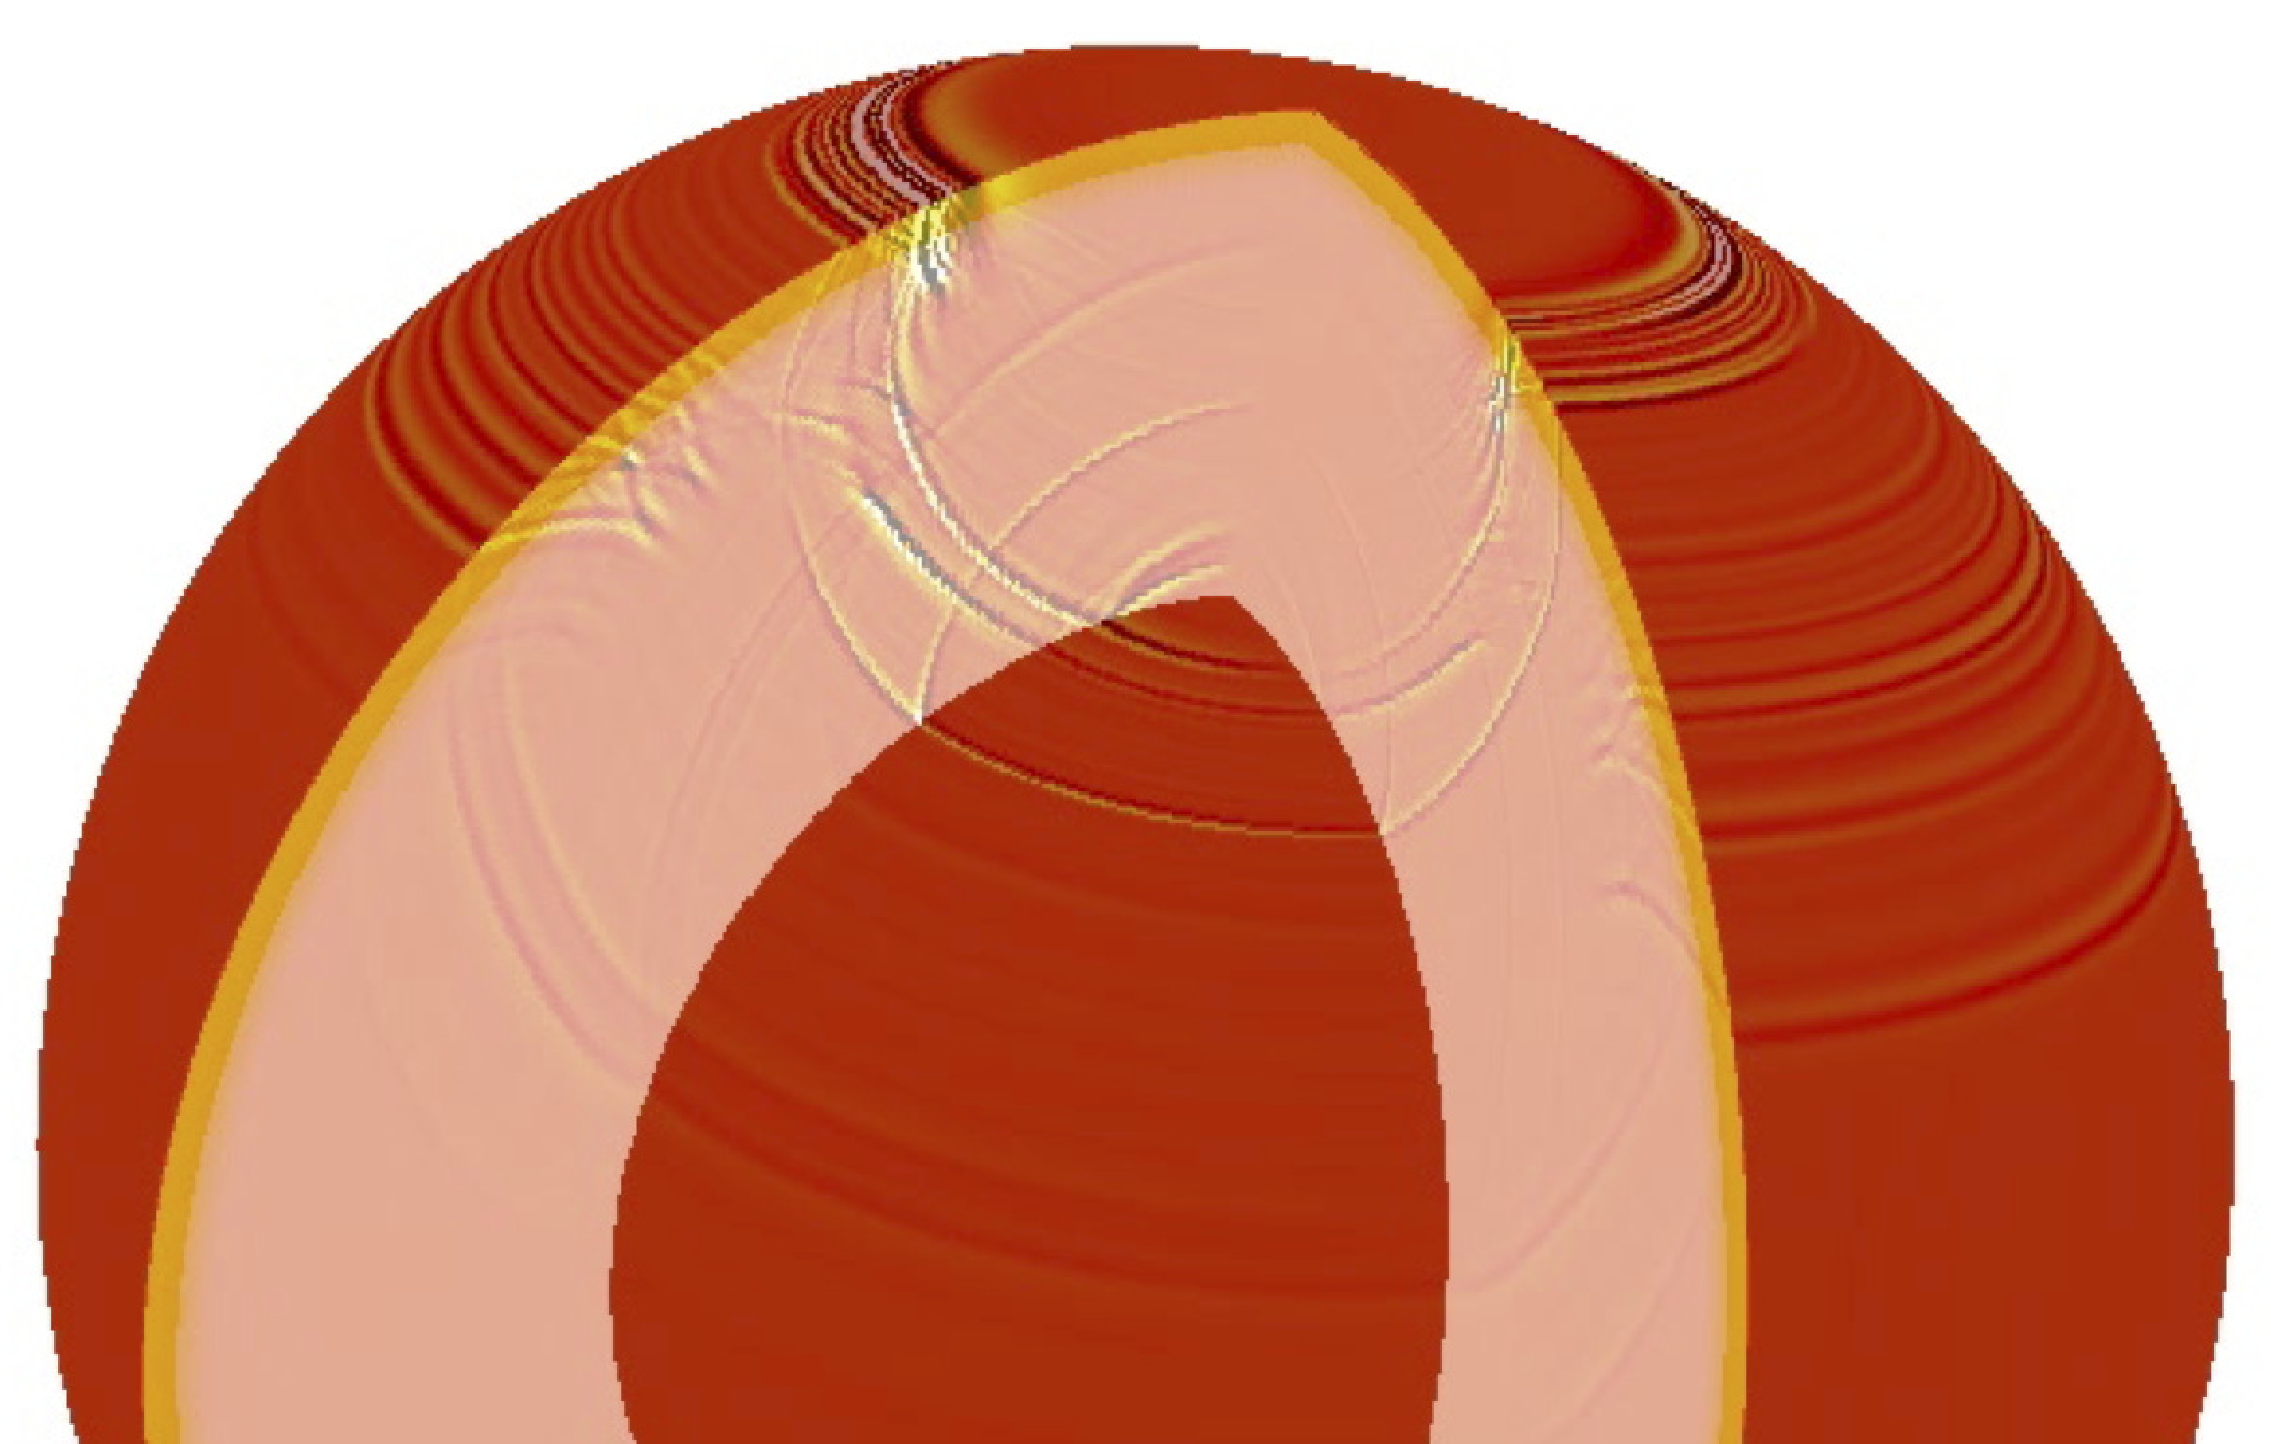
\includegraphics[width=0.9\linewidth]
{snap_cover_red.eps}}\end{picture}}
\vspace*{1.6cm}
\noindent {\sc AXISEM} is a \textbf{parallel spectral-element method} to 
solve 3D wave propagation in a sphere with
axisymmetric or spherically symmetric visco-elastic,
acoustic, anisotropic structures. Such media allow the computational
domain to be collapsed to a 2D disk, where the third, azimuthal
dimension is solved analytically on-the-fly posteriori. This
leads to extreme speedup by many orders of magnitude with respect to methods that discretize the
3D domain, and enables a full coverage of the seismic body- and
surface wave frequency spectrum between 0.001-1Hz. 
The time-domain code delivers full spatio-temporal wavefields that can be stored on
disk and transformed to frequency domain. Due to the dimensional reduction, global 
wave propagation at typical seismic of \textbf{periods down to 5 
seconds can be tackled on laptops}, and at 1Hz on moderate clusters.

%Exploitation 
%of moment-tensor source and single-force radiation patterns allow the \textbf{computational domain 
%to be collapsed to a 2D semi-disk}, and the azimuthal third dimension is computed analytically.
%For each full earthquake moment tensor (single-force vector), 4 (2) simulations are undertaken that account for 
%tensor (vector) elements separately and are summed subsequently.
The Fortran 90 code is divided into a \textbf{Mesher}, a \textbf{Solver} utilizing the message-passing interface 
(MPI) for communication between separate domains, and
\textbf{extensive post processing} for ease of visualization.
%Radiation pattern symmetries require all sources 
%to be located along the axis, and any lateral heterogeneities are translated into a 2.5-dimensional
%ring-like structure.
The essential raison-d'\^{e}tre of this method is the \textbf{efficient calculation 
of seismograms, wavefield movies, and those wavefields that underly
sensitivity kernels} to allow for tomographic inversions of any portion of a seismogram at any relevant 
frequency. \\
%We have added methodological foundations directly extracted from the references.
%Eventually, we will add the sensitivity kernel software as well. \\

\noindent Provisional portal for this code at ETH Zurich:
\url{https://svn.seismo.ethz.ch/trac/axisem/}\\
Please contact Tarje (\url{tarjen@ethz.ch}) for login information.

\section{Authors, contributors \& copyright}
%
\noindent \textbf{Principal authors:} Tarje Nissen-Meyer, Alexandre
Fournier, Martin van Driel\\
\noindent \textbf{Contact:} Tarje Nissen-Meyer (\url{tarje@alumni.princeton.edu})\\
\noindent \textbf{Contributions:}
 J.-P. Ampuero, E. Chaljub, A. Colombi, F. A. Dahlen, S. Hempel,
 K. Hosseini, D. Komatitsch,
 G. Nolet, K. Sigloch, S. St\"{a}hler, J. Tromp.\\
\noindent \textbf{Research funding:} Princeton University, NSF (USA), SNF (Switzerland), and 
ETH Zurich.\\
\noindent \textbf{Guarantees:} No guarantee whatsoever is given for this software under any circumstances. It may be used freely for 
academic purposes under the GNU license. Commercial use must be
discussed with the authors prior to usage.\\

\noindent \copyright  \hspace*{0.1cm} 
2007-2013 Tarje Nissen-Meyer (\url{tarje@alumni.princeton.edu}), ETH Zurich

\newpage
\tableofcontents
\newpage

\section{Preliminaries}

\subsection{Software and hardware requirements}

\textbf{Essential requirements:} 
\begin{itemize}
\item \textit{Compilers:} Fortran 90 compiler (tested on ifort, gfortran, pathscale)
\item \textit{Libraries:} MPI (tested on OpenMPI, mpich)
\item \textit{Systems:} Unix-based OS (tested on 32/64 Bit Linux clusters,
  Dell Nehalem, OS X.4-7,  Cray XT4)
\end{itemize}

\textbf{Optional embedded software/libraries:} netcdf, fftw3, python, taup, gnuplot

\textbf{Optional processing software:} xmgr, matlab, paraview, google earth
\subsection{References}

\noindent \textbf{Directly dealing with this code:}\vspace*{0.2cm}

(1) Tarje Nissen-Meyer, F. A. Dahlen, A Fournier (2007),
\textit{Spherical-earth Fr\'{e}chet sensitivity kernels},        
Geophysical Journal International 168(3),1051-1066. 
doi:10.1111/j.1365-246X.2006.03123.x                \\
                                                        
(2) Tarje Nissen-Meyer, A Fournier, F. A. Dahlen (2007), 
\textit{A two-dimensional spectral-element method for
spherical-earth seismograms-I. Moment-tensor source}, 
Geophysical Journal International 168(3), 1067-1092. 
doi:10.1111/j.1365-246X.2006.03121.x                 \\
                                                       
(3) Tarje Nissen-Meyer, A Fournier, F. A. Dahlen (2008),  
\textit{A two-dimensional spectral-element method for   
spherical-earth seismograms - II. Waves in solid-fluid media},
Geophysical Journal International, 174(3), 873-888.
doi:10.1111/j.1365-246X.2008.03813.x\\

(4) Tarje Nissen-Meyer (2007),
\textit{Full-wave seismic sensitivity in a spherical Earth},
Ph.D. thesis, Princeton University
(This includes refs (1)-(3) and more details.)\\

(5) Jean-Paul Ampuero, Tarje Nissen-Meyer (2011),
\textit{High-order conservative time schemes in spectral-element methods 
for seismic wave propagation.}, To be submitted to Geophys. J. Int.\\

\noindent \textbf{NOTE:} Most important sections of these papers are in the Theory section below.\\

\noindent \textbf{Other references:}\vspace*{0.2cm}

(6) Deville, M. O., Fischer, P. F., Mund, E. H. (2002), 
\textit{High-Order Methods for Incompressible Fluid Flow}, 
Vol. 2, Cambridge monographs on Sppl. \& Comp. Math., Cambridge University Press.\\

(7) Tufo, H. M., Fischer, P. F. (2001), \textit{Fast Parallel Direct Solvers For Coarse Grid Problems}, 
61, 151-177, J. Par. and Dist. Comput.\\

(8) Bernardi, C., Dauge, M., Maday, Y. (1999), \textit{Spectral Methods for Axisymmetric Domains}, 
Vol. 3, Series in Appl. Math., Gauthier-Villars, Paris.\\

(9) Chaljub, E. (2000), \textit{Mod{\'{e}}lisation num{\'{e}}rique de la 
propagation d'ondes sismiques en g{\'{e}}om{\'{e}}trie sph{\'{e}}rique: Application {\`{a}} la sismologie globale}, 
Ph.D. thesis, Universit{\'{e}} de Paris 7.\\

(10) Komatitsch D., Tromp, J. (2002), \textit{Spectral-element simulations of global seismic wave propagation---{I. V}alidation},
149, 390-412, Geophys. J. Int.

\section{Overview}

\subsection{Minimalist approach}
This is the step-by-step, blackbox procedure, i.e. running a workflow from raw source code to analyzing 
seismograms and wavefield movies upon pre-set parameters.\\

\noindent \textit{Basic requirements}: gfortran and MPI compiled for gfortran.\\
\textit{Processing requirements (not obligatory)}: gnuplot, taup\\
\textit{Visualization tools (suggested):} paraview, matlab, googleearth\\

\noindent Start from within the {\tt AXISEM} directory:
\begin{enumerate}
\item {\tt cd MESHER}
\item {\tt ./makemake.pl} $\Rightarrow$ creates Mesher Makefile.
\item {\tt make clean; make} $\Rightarrow$ make sure {\tt xmesh} exists.
\item {\tt ./submit.csh} $\Rightarrow$ Check {\tt OUTPUT}.
\item Wait for ``{\tt ....DONE WITH MESHER}'' to appear in {\tt OUTPUT}.
\item {\tt ./movemesh.csh TEST\_MESH} $\Rightarrow$ moves mesh files to {\tt ../SOLVER/MESHES/TEST\_MESH}.
\item {\tt cd ../SOLVER}
\item {\tt cp MESHES/TEST\_MESH/mesh\_params.h .} $\Rightarrow$ defines the mesh as a header.
\item {\tt ./makemake.csh} $\Rightarrow$ creates Solver Makefile.
\item {\tt make clean; make} $\Rightarrow$ make sure {\tt xsem} exists.
\item {\tt ./submit.csh TEST\_SOLVER} 
\item {\tt cd TEST\_SOLVER} $\Rightarrow$ Check {\tt OUTPUT\_TEST\_SOLVER}.
\item Wait for ``{\tt  PROGRAM axisem FINISHED}'' to appear in {\tt OUTPUT\_TEST\_SOLVER}.
\item {\tt ./post\_processing.csh}
\item {\tt cd Data\_Postprocessing} 
\item {\tt googleearth}, open {\tt src\_rec\_processed.kml}, click earthquake (info), receivers (seismograms).
\item {\tt matlab}, run {\tt plot\_record\_section.m}, plotting all components of displacement seismograms.
\item {\tt cd SNAPS; paraview}, load snaps for 3D wavefield movie.
\end{enumerate}
Once this has been succesfully completed, steps 2., 3., 9. can be omitted. If the Solver is re-run with different parameters but the
same mesh, you may start at step 11. Changing mesh input is done between 3. and 4., changing solver input between 10. and 11.,
changing post-processing input between 13. and 14. Using a new mesh requires recompilation of the solver (step 10.). If post
processing parameters are changed, also change the post processing directory.

\subsection{General remarks on the codes}
\textbf{Overview.} 
AXISEM is a parallel spectral-element method of the Gauss-Lobatto-Legendre type to 
solve the 3D solid-fluid equations of motion in a spherically symmetric sphere. The Fortran 90 source 
code is divided into a Mesher and a Solver utilizing the message-passing interface (MPI) for communication
between separate domains. Due to symmetries in the earthquake radiation patterns, 
the 3D wavefield of an earthquake moment tensor is reconstructed from 4 separate simulations
within a 2D computational domain. This D-shaped cylindrical domain includes a non-physical boundary with
singularities at the symmetry axis which is accomodated by Gauss-Lobatto-Jacobi discretization and 
l'Hospital's rule and does not need to invoke any absorbing method. Due to this symmetry, earthquake 
sources need to be located along this axis, and any lateral heterogeneities in the background model 
would be seen in an effectively ring-like structure.\\
The essential raison-d'\^{e}tre of this method is the efficient calculation 
of seismograms, wavefield movies, and specifically wavefields that constitute the crux for 
sensitivity kernels to allow for tomographic inversions of any portion of a seismogram at any relevant 
frequency. The two main parts are the mesher to construct a 2D domain for a given number of processors, 
resolution and input background model, and the solver which conducts the temporal evolution of the system 
explicitely at arbitrary spatial and up to sixth-order temporal accuracy.\\

\textbf{Code structure \& coding philosophy}
\begin{itemize}
\item The $>$40.000 lines of code 
are very \textbf{modular} in nature, such that vast parts of the code shall never need to be seen by anyone 
wishing to change/add something. This is particularly the case for the intricate geometrical mapping relations, quadrature, 
spectral operations, interpolation, index-mapping in the mesher, and some of the I/O.
\item Check {\tt main.f90} in either code for an overview of the tasks. Most important routines are well documented 
(at least in the Solver case!)
\item The codes allow for single or double precision (specified in {\tt global\_parameters.f90}), but in any case, crucial 
geometric operations are done in double, whereas large wavefield arrays in single can reduce computational cost 
notably if chosen.
\item The Mesher allocates memory dynamically, whereas the Solver includes the major array sizes from the mesher into 
a header ({\tt mesh\_params.h}). This means that each new mesh requires recompilation of the Solver. 
\item Input options are few and physical: The aim is to streamline as much as possible and leave only those options that 
relate to practical choices.
\item All variables and constants that are needed across modules are defined 
in files named {\tt data\_xxx.f90}; global constants in {\tt global\_parameters.f90}.
\item Changes in any of the input files do NOT require recompilation, changes in 
{\tt *.f90} or {\tt *.h} files DO require recompilation. 
\item Standard output is written to files called 
{\tt OUTPUT} (mesher) and {\tt OUTPUT\_<solverdir>} (solver), 
which contain all relevant information regarding either run. 
\item Optimization: The solver runs fully on unit-stride cache access and unrolled loops for tensor products 
as well as asynchonous message passing. The relevant routines performing these tasks are few and very 
general, so any changes in performance should first have a look there.
\item Everything related to MPI and parallel worlds is confined to the module {\tt commpi.f90}. In order to completely 
debunk message passing, one simply needs to remove {\tt commpi.f90}, and change a few lines in {\tt commun.f90} (as 
indicated there), then restart the {\tt makemake.pl; make clean; make} workflow. 
\item Object-oriented fortran features have been ommitted almost entirely due to their severe negative impact on performance.
\end{itemize}

\subsection{General workflow}
The generic workflow for both Mesher and Solver is as follows:
\begin{enumerate}
\item {\tt ./makemake.pl <arguments>}
\item {\tt make clean; make}
\item Edit input parameters
\item {\tt ./submit.csh <arguments>}
\end{enumerate}

\noindent {\tt makemake.pl } generates the respective Makefiles. Argument \#1 options 
(check available options with {\tt ./makemake.pl -h}) include:
{\tt gfortran} and {\tt ifort}, argument \#2 is optional and only defined for {\tt debug}. Best is to try some options and 
check the Makefile to make sure it suits you.\\

\noindent \textbf{Input parameters: } Input ({\tt vi inparam\_mesh})
to the Mesher is simple, you should in most cases (of conventional earth models) 
not need to edit more than the first 3 parameters (earth model, seismic period, and number of processors). 
Input to the Solver is attempted to be streamlined to the most primitive basis of settings as well. General 
input parameters are set in {\tt inparam}, source and receiver parameters in separate files (specified 
in {\tt inparam}). The information from the mesh is confined to the header file {\tt mesh\_params.h} 
which needs to be copied into the source code directory \textit{prior to compilation}.\\

\noindent {\tt submit.csh} are scripts to submit the jobs, check details with {\tt ./submit.csh -h} for both Mesher and Solver. 
In both cases, one can choose the queuing system (so far lsf and torque/maui) via arguments. In the Solver case, the 
source radiation type can also be specified via arguments. Note that in the case of a full moment tensor, 4 jobs will 
be submitted, and in the case of a full force vector 2. The script for the solver performs a variety of crucial operations 
for the simulations to succeed, act with sensitive care in case you really need to edit this script! \\

\noindent Upon successful completion of either job type, several post-processing options are available to indulge in. The 
mesher contains several vtk files to check the mesh via paraview, the solver contains a comprehensive and important 
series of operations invoked via {\tt ./post\_processing.csh } from the directory of the run. This includes 
summation over individual moment-tensor element responses, convolution with source time functions, rotation to 
actual source-receiver geometry, google-earth plots, seismograms in ascii and graphical formats, 
traveltime tables, 3D wave propagation snapshot movies, and a matlab script for plotting seismogram record sections.

\subsection{Algorithmic \& technical features}
\begin{itemize}
\item Global numbering scheme (P. Fischer \& H. Tufo)
\item High-order symplectic time integration schemes (co-developed with Jean-Paul Ampuero)
\item Unit-stride cache access, unrolled matrix products (Deville, Fischer, Mund)
\item Asynchronous (non-blocking) message passing (Tufo)
\item Output in VTK cell geometry
\item netcdf, xdmf file formats
\item python interface 
\end{itemize}

\subsection{File formats}

\subsection{Automated testing}

This section is mainly useful for the develpers or those want to change/add/remove some parts of the code and compare the new changes with the reference solutions.
For the reference solutions, 5 different tests have been designed and 
the results from \textit{yspec} [Al-Attar \& Woodhouse (2008)] and AXISEM have been included in the \textit{TESTING/automatic} directory.
The whole procedure (running the code, compare the results and plot) is automatic with the least user intervention: \\

Start from within the {\tt AXISEM} directory:
 \begin{enumerate}
 \itemsep0em
 \item {\tt cd TESTING}
 \item {\tt python test\_axisem.py}
 \end{enumerate}

Enter test number(s) and this is all you should do! \\

\noindent As an example, we want to run the \textit{test\_axisem.py} for test number 5. (Figure~\ref{test_axisem})

\begin{figure*}[htb]
\begin{center}
\includegraphics[scale=0.4]{PYAXI/test_axisem.eps}
\caption{\textit{Screenshot while running test\_axisem.py}}
%\caption{\textit{}}
\end{center}
\label{test_axisem}
\end{figure*}

\noindent At the end, it plots three figures (one for each channel) 
in which the new AXISEM waveforms are compared with both the original ones and \textit{yspec} results for the same simulation.
%In Figure~\ref{channel_Z}, only the Z channel has been plotted.
It should be noted that these tests are designed for rough comparison purposes (in terms of the pulse shape and sign) and they should not be considered as a detailed benchmark with respect to YSPEC. \\

\begin{figure*}[htb]
\begin{center}
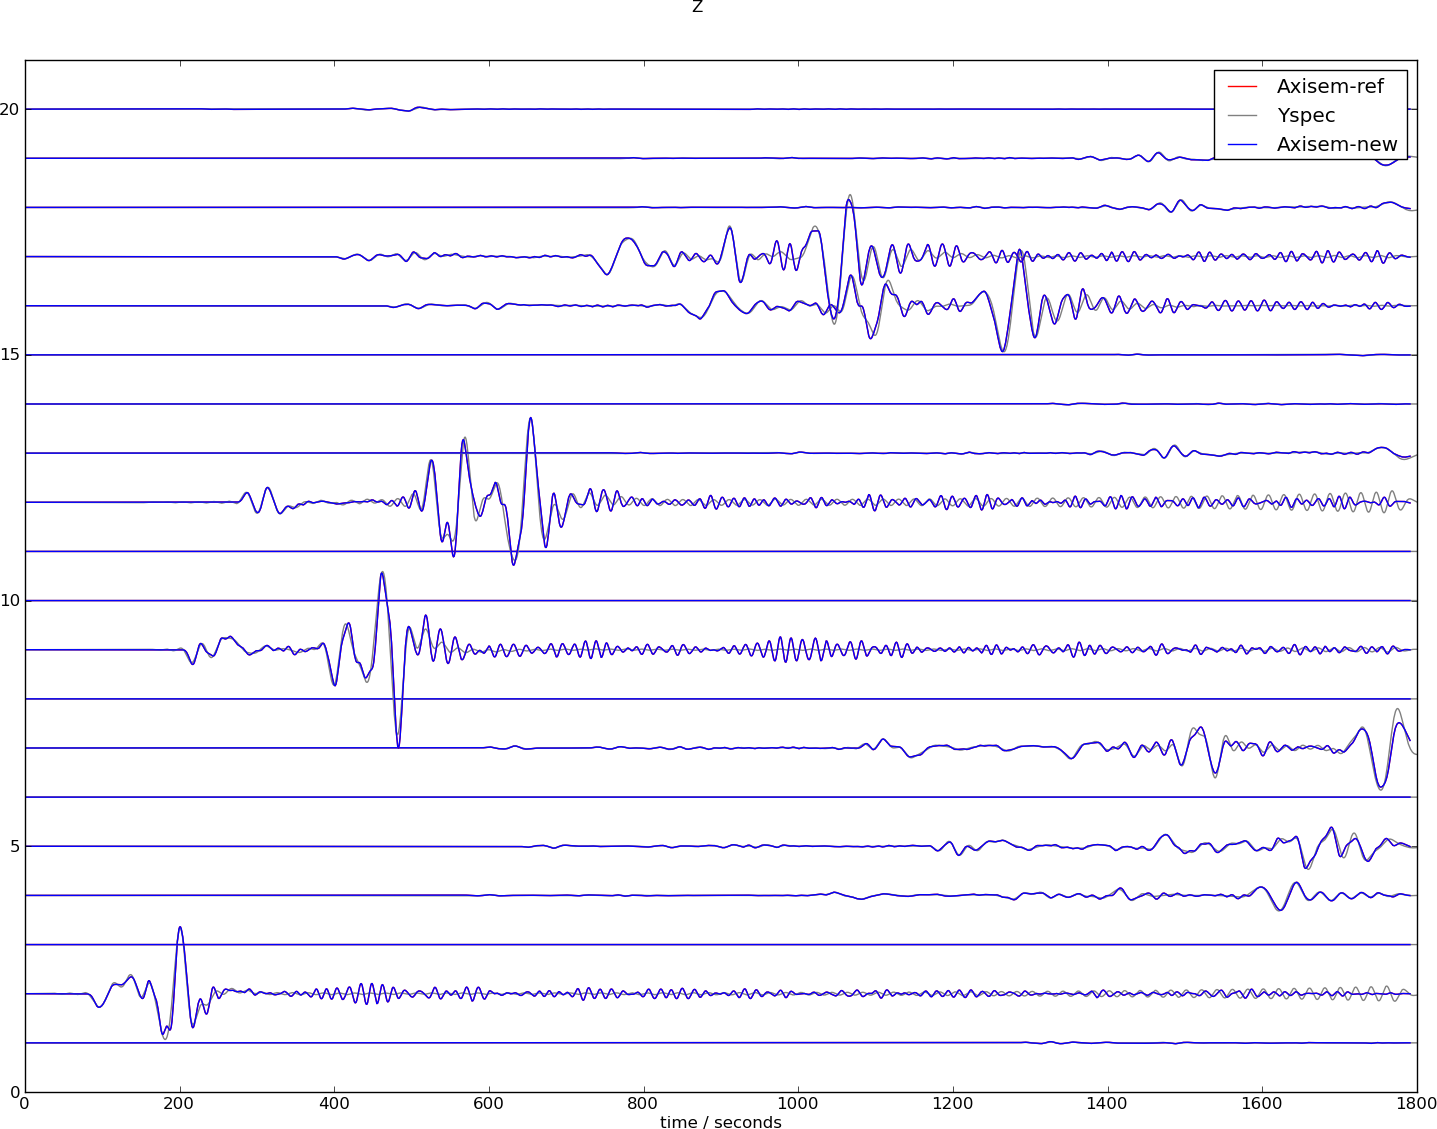
\includegraphics[scale=0.3]{PYAXI/record_section_Z.eps}
\caption{\textit{Comparing new AXISEM results with the reference solution and \textit{yspec} waveforms. (Z channel)}}
\end{center}
\label{channel_Z}
\end{figure*}

\noindent Another output is the \textit{l2} misfit (Figure~\ref{l2_misfit}) between the new and reference data 
in which the traces can be compared in a quantitative sense.

\begin{figure*}[htb]
\begin{center}
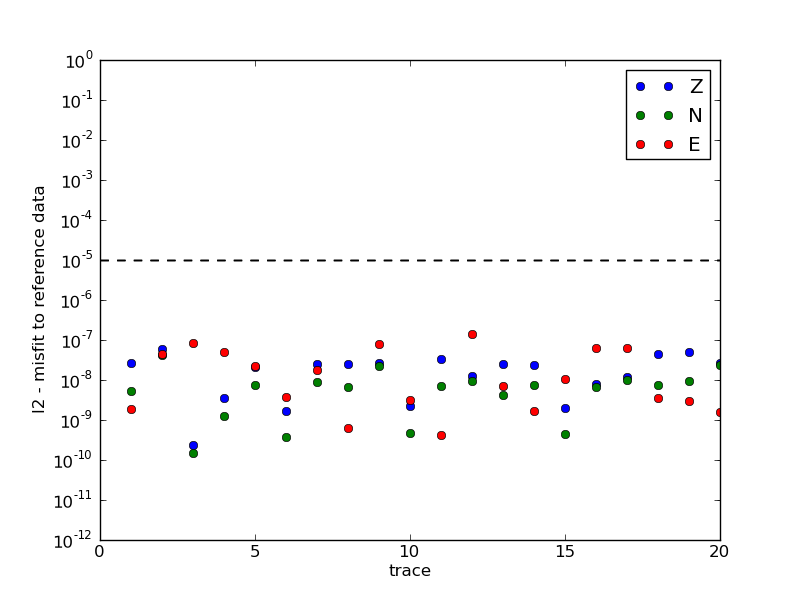
\includegraphics[width=0.8\textwidth]{PYAXI/l2_misfit.eps}
\caption{\textit{l2 misfit between the new and reference data.}}
\end{center}
\label{l2_misfit}
\end{figure*}


\subsection{Virtual box: 3-hour tutorial}

COMMENTS: (with permission, I (Kasra) highlight the important parts for next references)

* Tarje:
Hi Kasra, on a quick look, this seems excellent, but from my experience it’s better to have a very easy and quick first run of the tasks, e.g. on ONE page with all the important calls and major points we wish to achieve... and delegate images and details to an appendix. So, let’s keep all this in but reshuffle it to have a concise early section. Tarje

I would structure it as I said in the email... pasting it here again:
Tutorial:
1) 10min intro
2) 10min big run (maybe drop this, depending on progress next week)
3) 60min virtual box: data and AxiSEM
4) 20min big run post processing
5) installation of AxiSEM, obspy locally

(TAS÷
1) Load data from one of the 5 events (Kasra) with Obspy, plot cross sections
2) change AxiSEM input parameters to run this scenario, submit job
3) check mesh, background model, source-receiver geometry (google earth)
4) run post processing, filter, sum, movie snapshots
5) Movie snapshots
6) plot data vs. synthetics
7) plot AxiSEM synthetics vs SPECFEM
8) change input parameters (source CMT), load run with different background model

The virtual box should therefore contain:
(DONE)        - all 5 events (metadata and data), each in one directory 
(PENDING) - AxiSEM source code structure (mesher, solver, manual, testing)
(DONE*)       - all axisem runs replicating the data for 2-3 background models and source choices
(PENDING)  - plots of seismograms, movie 
*: for each event there are: prem\_aniso and iasp91 for 5 (PENDING),10,50,100 seconds



AXISEM vs DATA:


Start from within the SCRIPTS directory:
1. python sta\_event\_plot.py ../EVENTS/EVENT-1: plot the event and all the stations in the selected directory (EVENT-1 in this example).
2. run AXISEM for one of these events. The required information is located in /EVENT-1/INFO.
3. 



































% 1. Introduction
% In this part of the tutorial, we want to compare AXISEM waveforms with real data. For this reason, three events are selected (Figure 1). Detailed information for each event can be found in APPENDIX-1.


% Figure 1: beach ball diagrams (based on GCMT catalog) of event-1 to event-3

% Figure-2 shows how these events and their meta-data are organized in the Virtual-box.

% ?????????????????SHOUDL BE ADDED?????????????????????
% Figure 2: folder structure

% In SCRIPTS directory, two python scripts are provided that we will use here:
% 1. epi_plot.py: plotting tool for comparison purposes.
% 2. tt_plot.py: project the time shift derived by cross correlating the AXISEM waveforms and real data.

% 2. Run AXISEM
% As the first step, we want to simulate event-2 (Figure-3) with AXISEM. All the required AXISEM input files are provided in ????folder???.  APPENDIX-2 gives a quick overview on how to run AXISEM using PyAxi (Python interface for AXISEM).

% Figure 3: event and station configuration for event-2

% Once your simulation is done, all the AXISEM synthetic waveforms should be moved to ????folder???:
% cp <synthetic_waveforms> <destination????>

% 3. Compare the results
% To have an idea on how the synthetic and real data look like:
% python epi_plot.py ????address???


% Figure 4: AXISEM and real data waveforms arranged by epicentral distance

% For one specific seismic phase (Pdiff in this example), the following command plots the results of AXISEM against the real data: (to change the frequency?????)
% python epi_plot.py ../EVENTS/EVENT-2/AXISEM_PRE_SIMULATED/PREM\_ANISO_5sec/ Pdiff

% Figure 5: AXISEM and real data waveforms arranged by epicentral distance (Pdiff seismic phase)

% SPECFEM3D waveforms can be also added to the comparison by: (how to retrieve SPECFEM?!?!?!?!?)
% python epi_plot.py ../EVENTS/EVENT-2/AXISEM_PRE_SIMULATED/PREM_ANISO\_5sec/ Pdiff specfem3D
% Figure 6: AXISEM, SPECFEM3D and real data waveforms arranged by epicentral distance (Pdiff seismic phase)


% 4. Travel time measurements
% The time shift between AXISEM and real data (Figure 5) can be roughly measured by cross-correlating the time series. epi_plot.py can perform this and shift the synthetics in order to match them up:
% python epi_plot.py ../EVENTS/EVENT-2/AXISEM_PRE_SIMULATED/PREM_ANISO_5sec/ Pdiff shift_synthetics

% Figure 7: AXISEM and real data waveforms arranged by epicentral distance (Pdiff seismic phase), synthetic waveforms are shifted based on cross-correlation analysis.

% The calculated time shift can be mapped on the relevant station for the selected phase:
% python tt_plot.py ../EVENTS/EVENT-2/

% APPENDIX-1: Events
% ????????

% APPENDIX-2: A Quick Guide to PyAxi
% PyAxi (Python interface for AXISEM) is a Python script to run AXISEM automatically.

% python PyAxi <inpython.cfg> <STATIONS>

% and the rest should be done automatically. Therefore, to run the AXISEM for the provided examples (I mean! AXISEM_pre_simulated), it is enough to run:


% APPENDIX-3: Retrieving SPECFEM3D seismograms


% Event-1:
% ./obspyDMT.py --datapath EVENT-1 --min_date 2009-07-15 --max_date 2009-07-16 --min_depth 20 --list_stas /home/hosseini/Desktop/ALASKA_VBOX_LATEST/EVENTS/EVENT-1/INFO/STATIONS --specfem3D --offset 3600 --min_mag 7.0 --req_parallel --arc N

% Event-2:
% ./obspyDMT.py --datapath EVENT-2 --min_date 2009-09-30 --max_date 2009-10-01 --min_depth 70 --list_stas /home/hosseini/Desktop/ALASKA_VBOX_LATEST/EVENTS/EVENT-2/INFO/STATIONS --specfem3D --offset 3600 --min_mag 7.0 --req_parallel --arc N

% Event-3:
% ./obspyDMT.py --datapath EVENT-3 --min_date 2006-10-15 --max_date 2006-10-16 --min_depth 20 --list_stas /home/hosseini/Desktop/ALASKA_VBOX_LATEST/EVENTS/EVENT-3/INFO/STATIONS --specfem3D --offset 3600 --min_mag 6.0 --req_parallel --arc N


\subsection{PyAxi: Python interface for AXISEM}

\subsection{Introduction}
PyAxi is a Python script developed as an interface for AXISEM. 
All the options available in AXISEM are included in only one input file (\textit{inpython.cfg}).
By running the script, all the necessary steps (MESHER, SOLVER and Post-Processing) will be done automatically.
Python is the only requirement; However, some special functionalities (mseed format, plotting in Python environment) need \textit{ObsPy} to be installed. \\

\noindent \textit{Basic requirement}: Python.\\
\textit{Convert to MSEED (not obligatory)}: ObsPy (https://github.com/obspy/obspy/wiki).\\

\subsubsection{How to Run PyAxi?}
%In this part, we show how to run PyAxi for different input files.
First, let's check whether AXISEM can be run properly on our machine. 
For this reason:\\

Start from within the {\tt AXISEM} directory:
\begin{enumerate}
\itemsep0em
\item {\tt cd TESTING}
\item {\tt python PyAxi.py --check}
\end{enumerate}
\noindent This gives an overview of the installation status of all relevant compilers and tools required
to run AXISEM on your machine (Figure~\ref{check_pyaxi}). 
Please note that \textit{--check} does not check for all the possible compilers.
It just checks for those listed in Figure~\ref{check_pyaxi}; 
therefore, for other compilers, it should be done manually.\\

\begin{figure*}[htb]
\begin{center}
\includegraphics[scale=0.32]{PYAXI/check_pyaxi.eps}
%\caption{\textit{}}
\end{center}
\caption{\textit{Checking all the relevant compilers and tools required to run AXISEM.}}
\label{check_pyaxi}
\end{figure*}


\noindent After installation of all required packages, 
maybe the best way to get familiar with AXISEM is to run the code with the default input file:\\

Start from within the {\tt AXISEM} directory:
\begin{enumerate}
\itemsep0em
\item {\tt cd TESTING}
\item {\tt python PyAxi.py inpython.cfg}
\end{enumerate}

All the rest will be done automatically...\\

\noindent \textit{inpython.cfg} is a configuration file that contains all the AXISEM options.
To change the input file, open \textit{inpython.cfg} with an editor:\\

Start from within the {\tt AXISEM} directory:
\begin{enumerate}
\itemsep0em
\item {\tt cd TESTING}
\item {\tt (editor) inpython.cfg}
\end{enumerate}


%%%and it has been divided into several parts:
%%%\subsubsection{general}
%%%This section in \textit{inpython.cfg} is dedicated to how and where you want to run the code.
%%%\begin{itemize}
%%% \item \textbf{address} is the directory where you have the AXISEM code.
%%% \item \textbf{mesh\_name} is the name of the directory in which the info of the generated mesh will be stored.
%%% \item \textbf{solver\_name} is the name of the directory in which the final solution will be stored.
%%% \item \textbf{verbose} produces verbose output on the screen (recommended for debugging).
%%% \item \textbf{new\_mesh} has three possibilities.
%%%'Y' runs all steps of AXISEM from generating the mesh up to saving the waveforms.
%%%'N' uses the available mesh and continues the code.
%%%'M' gives this possibility to the user to manually change the options listed at the end of the \textbf{general} section.
%%% \item \textbf{post\_processing} perferms the post processing step automatically.
%%%\end{itemize}
%%%
%%%\noindent Please note that these options make it possible for the user to change the work-flow as it is required.
%%%For instance, if you already have done one simulation and you want to use the same mesh for another simulation,
%%%it is enough to set $new\_mesh = N$.
%%%
%%%\subsubsection{mpi\_netCDF}
%%%mpi\_netCDF options control the make flags and netCDF functionality.
%%%\begin{itemize}
%%% \item \textbf{make\_flag} adds required flag(s) for running the \textit{makemake.pl} in both MESHER and SOLVER.
%%% \item \textbf{mpi\_compiler} could be set based on your local machine. 
%%% \item \textbf{netCDF} generates one netCDF file instead of having binary output.
%%% \item \textbf{netCDF\_LIBS} and \textbf{netCDF\_INCLUDE} should be changed according to your netCDF installation.
%%%\end{itemize}
%%%\subsubsection{mesher}
%%%Major options that control the MESHER part of AXISEM have been included in this part.
%%%For more information about \textbf{model}, \textbf{period} and \textbf{no\_proc} please refer to Mesher input section.
%%%
%%%\subsubsection{solver}
%%%In this part, first we have three options \textbf{no\_simu}, \textbf{seis\_length} and \textbf{time\_step}
%%%that are identical to \textbf{number of simulations}, \textbf{seismogram length} and 
%%%\textbf{time step} defined in Solver input. Moreover:
%%%\begin{itemize}
%%% \item \textbf{source\_type} could be selected from 'sourceparams' and 'cmtsolut'.
%%% \item \textbf{receiver\_type} has three 'colatlan', 'stations' and 'database' options.
%%% \item \textbf{save\_XDMF} saves XDMF files (high resolution 2D wavefields), more options in \textit{inparam\_xdmf}.
%%% \item \textbf{force\_aniso} for anisotropic model handling.
%%%\end{itemize}
%%%\noindent Based on what we have selected in 'source\_type', one of the two parts for the source parameters
%%%should be modified, e.g. if you have chosed 'cmtsolut', then go to the \textit{cmtsolut} parameters and 
%%%change the options accordingly.
%%%\subsubsection{post\_processing}
%%%This section controls the required options for Post processing. All the parameters are identical to what has been explained in \textit{Post processing} section.
%%%\subsubsection{MISC}
%%%MISC contains the input parameters for converting the waveforms to MSEED format and convolve them with Source Time Function.
%%%These parameters are optional and need \textit{ObsPy} to be installed.
%%%\begin{itemize}
%%% \item \textbf{mseed} to convert all the seismograms to MSEED format (one file for each).
%%%These files will be located in the SEISMOGRAMS/MSEED folder in each solution directory (\textit{solver\_name}).
%%% \item \textbf{mseed\_all} to convert all the seismograms into MSEED format (one file for all).
%%%It will generate one 'seismograms.mseed' file saved in SEISMOGRAMS folder. 
%%% \item \textbf{convSTF} convolves the converted seismograms with Source Time Function (STF).
%%% \item \textbf{halfduration} determines the halfduration of the STF.
%%% \item \textbf{filter} applies a lowpass and a highpass filter with the minimum and maximum
%%%frequencies defined in \textbf{fmin} and \textbf{fmax}.
%%%\end{itemize}
%%%\subsubsection{test}
%%%This part of the input file is just for the TESTING functionality that we have in AXISEM.
%%%In normal runs, one should keep the \textit{'test'} flag to 'N' to avoid any problem.
%%%TESTING will be discussed in a seperated section.



\newpage
\section{Mesher}
Constructs the spherical 2-D semi-disk of spectral elements based 
on a given background model, a target resolution as defined by 
the (dominant) source period, the number of processors, 
and the polynomail order of the spectral elements. 
This mesher is NOT well documented and rather involved regarding index mapping, 
hence subject to future streamlining efforts. Please let us know if you intend to add comments or 
change code to join forces.
It invokes a series of dingy, multiply layered bookkeeping index arrays that 
are not easy to follow (see mind-twisting highlights in {\tt parallelization.f90} and {\tt pdb.f90}). 
Again, we welcome improvements here but want to caution users to change 
anything if not entirely sure about all dependencies.\\

\noindent NOTE: The mesher is serial but constructs the parallel mesh database 
needed in the solver (in {\tt pdb.f90}), easily down to periods of about 
3 seconds on typical shared RAMs ($\sim$ 2GB). 
For higher resolutions on such chips, reordering of global variables and/or complete 
parallelization of the Mesher is a mundane task for $t>{\rm today}$.

\subsection{Installation and compilation}
Use {\tt ./makemake.pl <arguments>} to create the Makefile when opening for the first time or adding modules. 
Invoking {\tt ./makemake.pl -h} provides options for different compilers. Always check the resultant {\tt Makefile} to make 
sure it rocks, compiler- and flag-wise. Compile via {\tt make clean; make}. The executable is called {\tt xmesh}. 
Changing code without adding modules does not require to recreate the Makefile, only recompilation.

\subsection{Input}
\begin{figure*}[htb]
\begin{center}
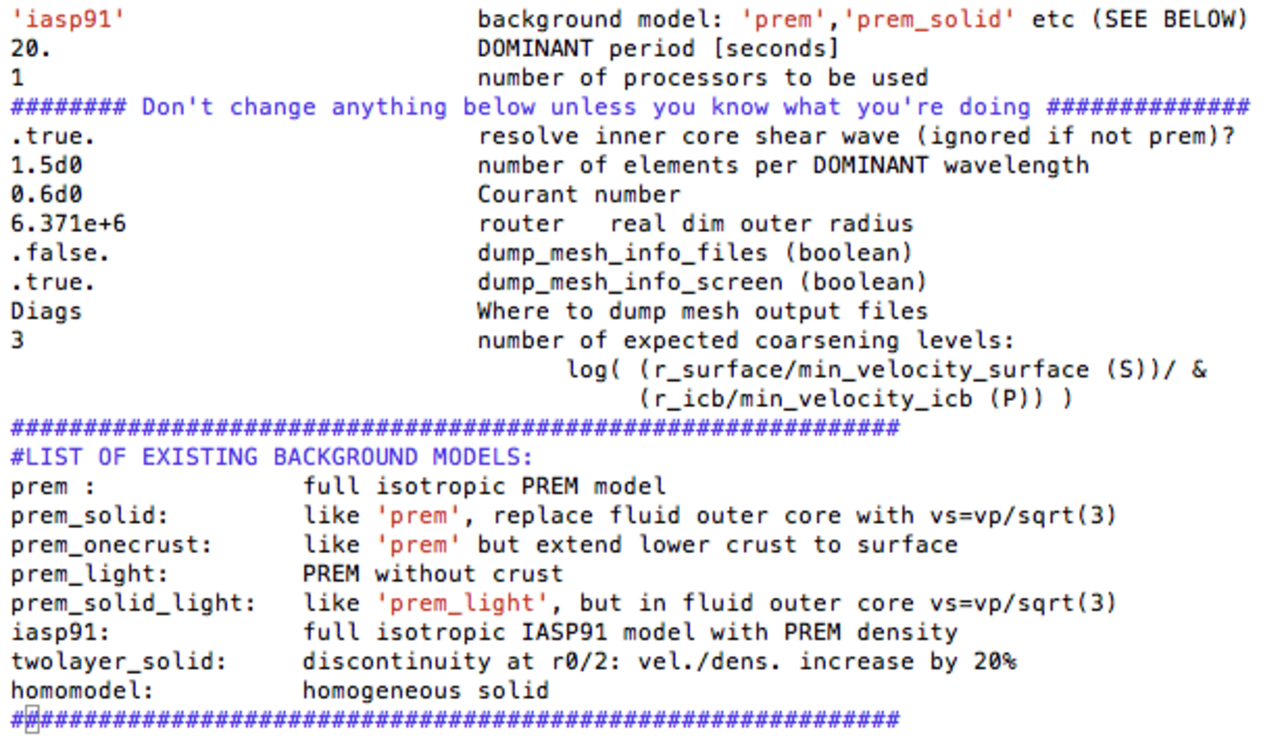
\includegraphics[scale=0.6]{inparam_mesh.eps}
\caption{\textit{{\tt inparam\_mesh}: defines all relevant parameters, mostly self-explanatory. }}
\end{center}
\end{figure*}

\noindent \textit{Basic set of parameters} to be edited:
\begin{itemize}
\item \textbf{background models}: Be sure that the string defined here exists in 
{\tt background\_models.f90}. Adding new background models is explained further below.

\item \textbf{dominant period:} This is the seismic source period at which dominant parts 
of the spectrum are propagated. Note that this is different from other codes in which the 
maximal frequency may be specified. 
In most applications, the solver should be run using a Dirac 
delta function and then convolved a posteriori with the source-time function (STF). In that 
case the pure simulation results contain high-frequency numerical noise beyond the mesh 
resolution, but the convolution eradicates those (even better than if a non-white spectrum 
STF is inserted as the source, since the spatial point source also introduces aliasing, which 
can only be taken care of via the above-mentioned posteriori convolution.

\item \textbf{number of processors}: needs to be a multiple of 2. At this point, the mesher 
only accomodates meshes up to 16 processors. This is not a serious limit, but 
merely a matter of having not implemented the central region decomposition 
for larger numbers (which shall not be necessary considering hardware developments).
\end{itemize}
\newpage
\noindent \textit{Advanced set of parameters} to be edited:
\begin{itemize}
\item \textbf{resolve inner shear wave:} This should always be set to true. If false, then the inner core 
is assumed fluid but the saved CPU cost is negligible.

\item \textbf{polynomial order}: The polynomial order $N$ of the Gauss-Lobatto-Legendre (GLL) basis 
within elements
is often said to be optimal at 4. However, this can be freely chosen, specifically if convergence tests are needed,
and Ref (5) suggests that higher polynomial orders may be more cost-effective, depending on the constraints 
imposed by the element mesh (e.g., thin crustal layers to be accomodated). The ``optimal'' judgment stems 
from the fact that the minimal spacing of GLL points depends on $1/N^2$, that is, the spectral convergence 
is counteracted by a possibly quadratic decrease in the critical time step.

\item \textbf{number of elements per wavelength}: This will be used to compute the largest
allowable grid spacing based on the dominant source period and is intimately 
tied to the polynomial order $N$. See ref (5) for 
a comprehensive analysis on how to choose the parameters if necessary.
If the seismograms contain unreasonable noise (usually high-frequency tails), 
are inaccurate or otherwise different than a reference solution or data, 
try to increase this value. This will result in a denser mesh at higher 
simulation cost (possibly more processors), but deliver more accurate results. 
The absolute minimum number of grid points per maximum wavelength for S waves 
is about 4.5 (i.e., this parameter times $N$). See ref (3) and (5) for details.

\item \textbf{Courant number}: Defines the stability criterion to choose the critical time step.
0.6 is the heuristically determined maximal value for any realistic 
applications. If the solver explodes, decrease this number. Note that dispersion errors increase 
with propagation distances (counted in wavelengths), and for large distances one should  
choose a smaller time step than the critical one (which is the one suggested by 
the output of the mesher in {\tt mesh\_params.h}).

\item \textbf{outer radius}: This is the same for IASP91 and PREM, but should be changed accordingly 
if other models necessitate otherwise, or of course if other spheroidals are considered. 

\item \textbf{mesh info files}: These files become extravagantly large for high-resolution meshes 
and are not needed by the solver, nor by any of the current post-processing tools and as such should 
be kept .false. unless significant changes or issues within the mesher are emerging.

\item \textbf{mesh info screen}: This is extra output containing some more details on the meshing 
process, but equally to the large files unnecessary for any normal meshing procedure.

\item \textbf{dump directory:} The directory where most of the output is written. The posteriori 
{\tt movemesh} script moves all those files to the permanent mesh location.

\item \textbf{coarsening levels}: Keep this at 3 if applied to any typical earth models, as
this number reflects the overall change in velocity between the surface and the deep interior.
if the total global variation in wave speed is significantly different, 
other options may be convenient here. This applies to other spheroidals, homogeneous 
or simply layered models.
\end{itemize}

\subsection{Running the mesher}
Job submission is simple:\\
{\tt ./submit.csh <optional queuing system>},\\
where {\tt <optional queuing system>} can be {\tt lsf, torque} at this point. Check {\tt ./submit.csh -h} for 
options.

\subsection{Changing the background model}
This is traditionally the bottleneck of seismic code flexibility (in my very biased view)... so 
we've given considerable effort to making this task as primitive and decoupled from the 
rest of the code as possible. In principle, two options for new earth models exist: \\
(1) Parameterized, polynomial, piecewise continuous representation of wavespeeds $v(r)$,\\
(2) Discrete radial values of $v(r_i)$.\\

\noindent In principle, this should be entirely general such that you can dream up multiple fluid layers,
discretely layered earths or other planets, ridiculous velocity variations, 
however we have not completed the fully fluid sphere just yet. As soon as your new 
model affects the overall change in velocity between surface and maximal value at depth, you 
will have to change the number of expected coarsening levels in {\tt inparam\_mesh} as indicated there.\\

\noindent Two modules will need to be amended: {\tt model\_discontinuities.f90} and {\tt background\_models.f90}.
Note that {\tt background\_models.f90} is copied to the Solver by {\tt movemesh} 
such that additions will be automatically accounted for in the Solver. 

\subsection{Anisotropy}

\subsection{Attenuation}

\subsection{Computational aspects}
The simulations should be done within seconds to minutes for meshes above 5 seconds.
Note that doubling the resolution (half the period) results in a mesh that 
is 4 times larger and has about half the time step, i.e. the solver takes 
double the time at 4 times more processors. Increasing the number of 
processors while keeping resolution constant will slow the mesher insignificantly, 
but in most cases speed up the solver substantially, but not linearly
(the more message passing, the slower).
This mesher is completely serial but constructs the parallel mesh database 
needed in the solver (in pdb.f90), easily down to periods of about 
3 seconds on typical memory chips ($\sim$ 2GB), and down to 1 second on 
larger shared memories (e.g. 12GB).

\begin{table}[h]
\begin{tabular}{ccc}
period & max  \\
 T[s]  & nproc & memory [GB] \\
\hline
 50.0 &    8  &  $< 1$  \\
 25.0 &   12  &  $< 1$  \\
 20.0 &   16  &  $< 1$  \\
  9.0 &   32  &  $< 1$  \\
  4.4 &   64  &  $< 1$  \\
  2.2 &  128  &  $ 3.5 $ \\
  1.1 &  256  &  $13.0 $ \\
\end{tabular}
\end{table}

\subsection{Code structure and components}
Check {\tt main.f90} for the general code structure. Meshing of the spheroidal is confined to the module 
{\tt discont\_meshing.f90}. The inner cube contains a coordinate transformation (see Theory section), which 
is done in {\tt meshgen.f90}. The domain decomposition is accomodated by {\tt parallelization.f90}, and the 
parallel database generated in {\tt pdb.f90}. You may wish to avoid diving into these murky modules 
unless your curiosity exceeds that of an average coding geek, or you encounter an issue.\\

\noindent\textbf{Domain decomposition }\\
In {\tt parallelization.f90} we have an exactly load-balanced colatitudinal cake-piece decomposition 
for the outer spherical part of the mesh. The central, rectangular part is trickier. 
We employ a method that is based on the following principles:
\begin{itemize}
\item exact load balancing 
\item maximally 2 neighboring domains, i.e. each domain touches the axis
\item at least two elements thickness
\item spherical cake-piece decomposition as 'boundary condition'
\end{itemize}
Upon this, we construct the decomposition by approximating polynomials $s(z)$
of varying degrees. For the time being, this is only implemented up to 
16 processors, but no hard limitation. See the Theory section in this manual for details.

\subsection{Output}
\underline{Needed by solver} \\
{\tt mesh\_params.h}\\
{\tt meshdb.dat0000,...,meshdb.dat00$<$nproc-1$>$}\\
{\tt unrolled\_loops.f90}\\
{\tt background\_models.f90}\\

\noindent\underline{NOT needed by solver }\\
Everything else (mostly in directory {\tt Diags/}) including various global 
arrays such as valence.\\

\noindent {\tt mesh\_params.h}: \\
This is a header file that contains all the static array 
sizes for the solver such that it does not need to allocate (a lot of) 
memory dynamically. Specifically, it documents all revelant mesh input 
parameters commented at the top, and some output information such as 
time step at the bottom.  The inclusion of this header into the solver 
requires recompilation for each new mesh. This header includes 
mesh sizes and is identical for each processor due to the exact load balancing.
The last line is added by {\tt movemesh} and indicates the location of the mesh 
database. If you move the mesh, make sure to change this line accordingly!!
\\

\noindent {\tt meshdb.dat00*}: \\
These are the complete databases for each processor of the 
solver simulations. They contain the skeleton mesh, regions, boundary 
information (axis, free surface, solid-fluid boundary, processor boundary), 
and basically everything needed for a full simulation except for the 
source-receiver specification which is an input for the solver. \\

\noindent After these two crucial output file types are written, the mesher reloads them as a
simple test on some of their dependencies. More comprehensive tests are 
performed in the solver. \\

\noindent\textbf{\underline{Prepare files to be used in solver}}\\
Use the script {\tt movemesh} to transfer all relevant files to the directory ../SOLVER/MESHES. 
Using this script is crucial since it adds 
a line to the {\tt mesh\_params.h} header file to indicate the location of the large mesh 
databases.

\subsection{Mesher Post-processing/quality control }
\begin{figure*}[htb]
\begin{center}\label{fig:mesh_vp}
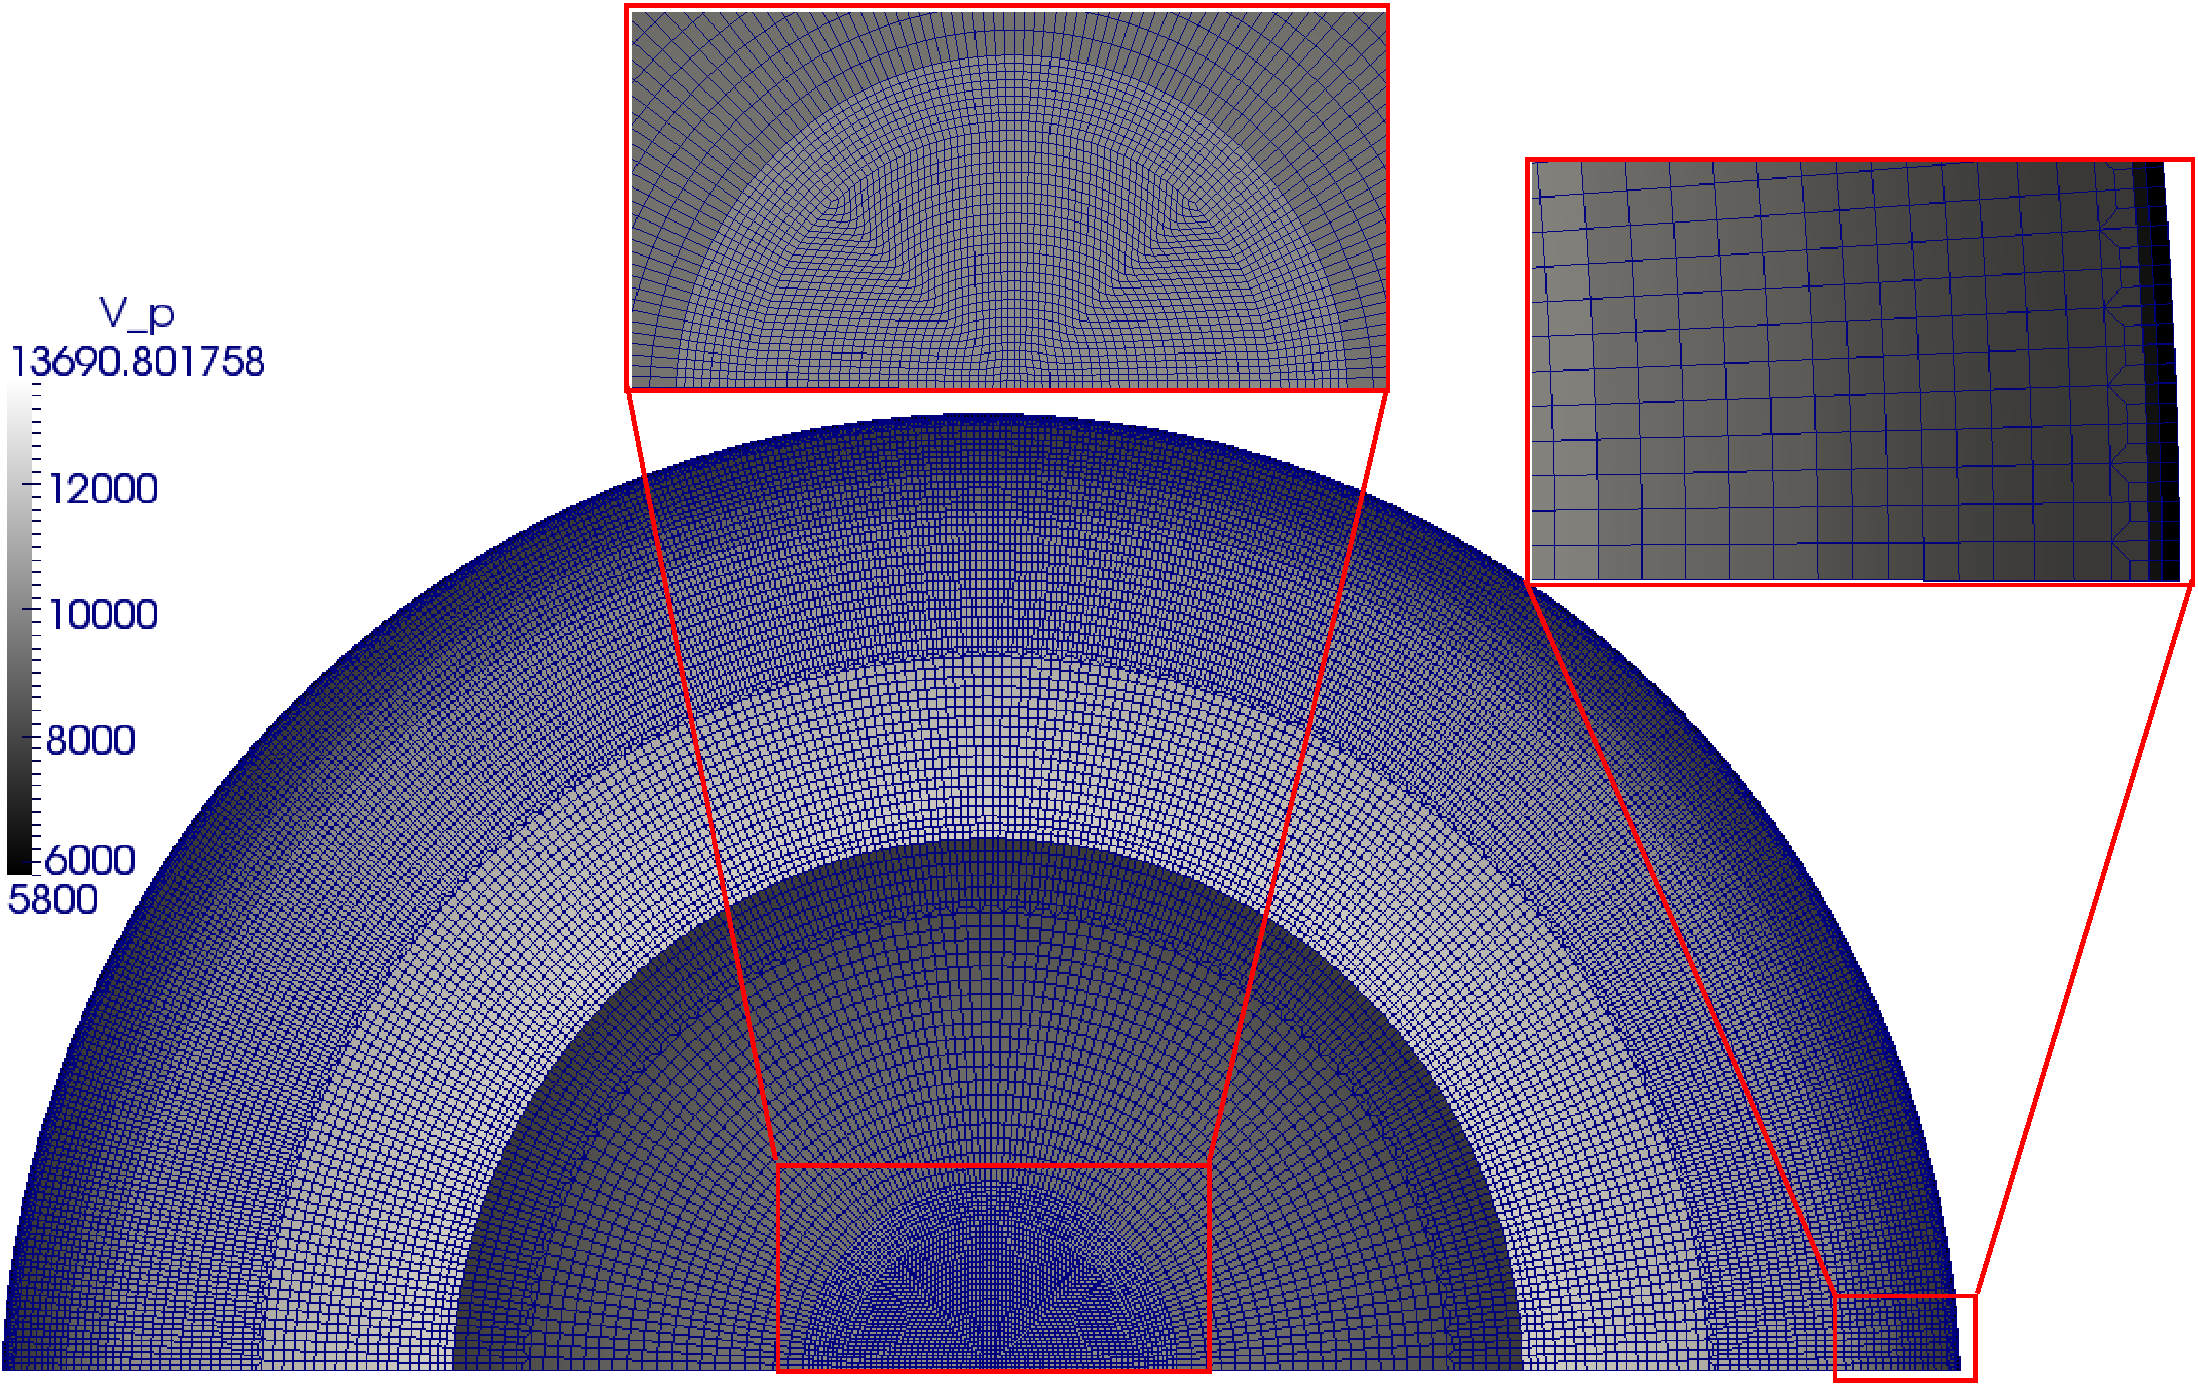
\includegraphics[scale=0.45]{mesh_vp_fig.eps}
\caption{\textit{The elemental mesh (blue lines) for IASP91 at 20 seconds superimposed on the $v_p$ velocity. 
The plot is derived straight from the file {\tt mesh\_vp.vtk} produced by the mesher. Zoom sections of the 
central region and crust/upper mantle are added to highlight the topological features.}}
\end{center}
\end{figure*}
%
\noindent Generic output includes various {\tt *.vtk} files on the elemental mesh with media properties 
(see Fig.~\ref{fig:mesh_vp}) as well as a host of other plots with respect to Courant number, 
points per wavelength, period, time step etc, and domain decomposition.
All of these files are moved to the permanent mesh location via {\tt movemesh} and can be easily viewed with {\tt paraview}. 
Turn on the \textit{surface with edges} and \textit{data} features to visualize the element mesh and medium 
properties, respectively.

\subsection{Cautions}
Fully operational in single or double precision, so please 
\textbf{avoid using the -r8 (enforced double precision) flag}, 
since the output expects single precision for certain arrays (especially in vtk).

\subsection{Issues}
The hmin/hmax vtk output files have strangely large values, but the period and dt ones are fine.

\subsection{Mesher To Do}
General cleanup, documentation, parallelization, domain decomposition in the central region for 
more than 16 processors, netcdf database.

\newpage
\section{Solver}
Picks up the header from the mesher into its compilation to solve 
the elastodynamic 3-D equations of motion for spherically symmetric 
earth models in a 2-D computational domain using message-passing for the 
parallelization. The full seismic moment-tensor $M_{ij}$ is accounted for by four
separate simulations: two monopole, one dipole, and one quadrupole 
simulation have to be done to sum up to the 6 independent elements of $M_{ij}$.
The software has the additional feature of computing and 
saving entire wavefields that form the basis of full-wave based, 
multiple-frequency sensitivity kernels. This output is included in the 
solver, but the calculation of kernels needs to be done elsewhere. 
Detailed information on the various components of the code are included as 
comments to the respective modules and routines. 
Here, we give a simple overview over the main parts. 
\newpage
\subsection{Installation and compilation}
\begin{enumerate}
\item If first used or new modules are added to the Solver code,
use {\tt ./makemake.csh } to create a new Makefile, see {\tt ./perlmakemake.pl -h} for 
flag options on different compilers. {\tt ./makemake.csh} checks for the
executable ncdump to determine whether your system supports netcdf. If
so, it includes netcdf library and include paths in the Makefile
(please check if they make sense!), and links the module that works
via netcdf in the solver. Still one can dump the output in other
formats, but the module including netcdf is simply used. In case
netcdf is not found, a ghost module is created instead to ensure
compilation. This will disallow usage of netcdf, quite obviously.
\item Copy {\tt mesh\_params.h} from the desired mesh into the source code directory: 
It contains a last line that links to the location of the database such that 
these possibly very large files do not need to be copied. 
\item Compile: {\tt make clean; make}
\item Make sure that executable {\tt xsem} exists.
\end{enumerate}

%\subsection{Pre-processing}
%The {\tt UTILS} directory contains some utilities that may be useful in 
%choosing the right input parameters. 

\subsection{Input}

\textit{Automatically taken from mesher:} \\
{\tt mesh\_params.h}: header including array sizes necessary for the compilation\\
{\tt meshdb.dat00\*}: mesh databases for each processor\\
{\tt unrolled\_loops.f90}: unrolled loops and unit-stride cache access for given polynomial order\\
{\tt background\_models.f90}: all background models. Needs to be the same as in mesher\\

\noindent Any changes to Solver code, background model, mesh, polynomial order etc. require 
recompilation. The above input files are fully automatic and need not be changed for all intents 
and purposes of the Solver.\\

\noindent \textit{Input files for the Solver:} \\
\noindent {\tt inparam, sourceparams.dat, receivers.dat}\\
These 3 solver input files may be changed without recompilation of the solver 
source code. We will describe these files at length in the following. PLEASE do not shy away from the 
length of this section.... the input is fairly easy to understand and manipulate, 
we simply intend to comment as much as possible on all options!\\

\begin{figure*}[htb]
\begin{center}
\includegraphics[scale=0.6]{inparam.eps}
\caption{\textit{{\tt inparam}: defines all relevant parameters, mostly self-explanatory. }}
\end{center}
\end{figure*}
%
\noindent {\tt inparam}:
\begin{itemize}
\item \textbf{number of simulations}: Keep this at 1 for the time being, this is not completed yet. 
If you wish to simulate full moment tensors or forces at once, do that via {\tt submit.csh}.
\item \textbf{seismogram length:} Useful to check this via a ray tracer (taup) before choosing, the overall 
CPU cost scales linearly with this length.
\item \textbf{time step}: If you keep this at 0.0, the code chooses the critical time step as specified in
{\tt mesh\_params.h}.
We suggest to choose a lower value than this critical value, at best some  
integer multiplicative of the seismogram sampling specified further below. The CPU cost 
scales inversely linear with the time step.
\item \textbf{time scheme}: see {\tt time\_evol\_wave.f90} for details. 
{\tt newmark2} is the traditional 2nd-order 
scheme, {\tt symplec4} is a PEFRL scheme of 4th order, about 2.5 more CPU time 
required than the Newmark scheme but significantly more accurate. See ref(5) for a
detailed analysis and rules of thumb for choosing the optimal time scheme. 
Generally, if the setup requires seismograms at more than 100 wavelengths 
in distance, we suggest using the symplectic scheme. The memory requirements 
for the symplectic scheme are in fact *lower* due to avoiding the acceleration
as a full wavefield. See the section on time schemes further below on more information.

\item \textbf{period}: Should keep this at 0.0 unless one wishes to test accuracy for 
constant mesh at varying frequencies, or somehow the simulations show 
inaccuracies. This choice is ignored if a delta function is used as the source 
time function (in {\tt sourceparams.dat}), which should be the preferred option
unless wavefield snapshots (for propagation movies etc) are needed. 
\item \textbf{source file type}: Functional choices are {\tt separate} and {\tt cmtsolut}.
{\tt separate} invokes the generic source file {\tt sourceparams.dat}, and {\tt cmtsolut}
the {\tt CMTSOLUTION} format. See next section for details on these files. 
\item \textbf{receiver file type}: Functional choices are {\tt colatlon} and {\tt stations}.
{\tt colatlon} invokes the generic receiver file {\tt receivers.dat}, and {\tt stations}
the {\tt STATIONS} format. See two sections down for details on these files. 
\item \textbf{seismogram sampling rate}: Keeping this at 0.0 saves seismograms 
at the time step sampling rate. Choosing values larger than the time step may 
be useful to maintain a sampling rate equal to that of, e.g., data. Note though 
that keeping this value too high will result in crude seismograms which loose 
valuable frequency information.

\item \textbf{data and info output paths}: We suggest to keep those as defined; 
{\tt Data} contains all the large output such as seismograms and wavefields and all 
associated information. {\tt Info} contains additional information files, e.g. on 
processor-specific output and properties. 

\item \textbf{Save global snapshots}: Saves the displacement wavefield at discrete time 
intervalls for posteriori compilation into a wave propagation movie. These files are LARGE!
Only needed for visualization, understanding certain wavefield features, but should be 
generally turned off. The post-processing scripts turn these wavefields into a 3D global 
wave propagation movie if saved. NOTE: if this is set to {\tt .true.}, then a Dirac delta 
source doesn't make sense since the spurious high-frequency signals cannot be filtered 
a posteriori. 

\item \textbf{snapshot time interval}: Time in seconds between frames for the above snapshots 
of the propagating global wavefield. Obviously the output size depends directly on this intervall... 
For decent movies we suggest to keep this at 1-2 frames per seismic period. 

\item \textbf{save wavefields for kernels}: So long as the kernel code is not available, this 
is pretty useless since the resultant wavefields are subjected to an extensive amount of operations 
(rotations, coordinate transformations, frequency-domain transformations, convolutions, filtering)
to arrive at sensitivity kernels. Setting this to false ignores the rest of the choices in this output 
section for sensitivity kernels. CAUTION: These files are gigantic for high resolutions!

\item \textbf{Samples per period}: Should be at least 2 to fulfill Nyquist, but more 
are highly recommended for the purpose of picking time windows when 
computing static kernels, e.g. 8-10.

\item \textbf{source vicinity in wavefields}: Sensitivity kernels exhibit large values right around 
the source and receiver. Apart from ignoring this ({\tt igno}), 
we offer the possibility to simply {\tt mask} this region with smaller values. 
An analytical calculcation for homogeneous regions is in the making.

\item \textbf{starting/ending GLL point index}: Option to save only select GLL points per element for the 
kernel wavefields. Choosing 1,1 means only interior points, which maintains a smooth sampling (due to the 
GLL point clustering near the element boundaries) and avoids the peculiar and tricky issue of defining 
numerically accurate strains on discontinuities.

\item  \textbf{energy}: avoid this unless you are specifically interested in the kinetic,
potential and total energy of the solid, fluid and global domains since it 
involves a full evaluation of the stiffness matrix and is therefore quite 
CPU (and memory) intensive. 

\item  \textbf{homogeneous parameters}: This is mainly for testing purposes and should be 
turned to false otherwise. Only possible for purely solid models 
and only really useful for testing/debugging.

\item \textbf{homogeneous P-vel etc}: Populates the entire domain with this 
homogeneous media characterization if exclusively solid.

\item \textbf{analytical solution around source}: An analytical reference solution to test the 
accuracy of near-source radiation in a homogeneous model. Should only be on if this is relevant.

\item \textbf{add heterogeneity}: Turning this {\tt .true.} invokes an additional input file called {\tt inparam\_hetero}. 
This perturbs the background model in a specified region (defined by elements within a range of specified coordinates) 
by percentile changes to velocities $v_p$, $v_s$, and density
$\rho$. This part of the code is still under development but contains
a number of different types of heterogeneties, all of which are
defined in {\tt lateral\_heterogeneties.f90}. See more details in the separate section below. 
This should generally be set to false unless you specifically wish to analyse waveform effects due to such 
2.5-dimensional heterogeneties. 

\item Setting the next two lines to false (do mesh tests, save large test files) 
avoids extensive checks on the mesh, model, discontinuities etc. Upon a new mesh, this may be turned 
to true at least once (same after any source code changes), otherwise
it's fine to avoid these tests and large files.

\item A new (Nov. 2011) feature is the I/O using the netcdf
  standard. This is extremely beneficial for platform-independent
  binaries, direct access, reducing the number of written files, and
  is installed on every well-managed computer cluster. However,
  installing these libraries can be tedious. For this case, we have
  left the option to go with fortran binary. The decision is two-fold;
  the first one already taken in {\tt makemake.csh} since the makefile needs to
  know whether the libraries are installed. Even if installed, one can
  still turn the netcdf option off by putting binary here. 
\end{itemize}

\noindent \textbf{Source specification.}\\
Includes all parameters describing the earthquake (or other) source, which are: 
radiation patterns and magnitude, source location (depth, latitude, longitude), source-time function.
As of now, the code only computes point sources (finite faults are in development), 
and simply takes the closest grid point as the location. Mislocation errors are given in OUTPUT\_$<$dir$>$.\\

\noindent {\tt sourceparams.dat}
\begin{figure*}[htb]
\begin{center}
\includegraphics[scale=0.6]{sourceparams.eps}
\caption{\textit{{\tt sourceparams.dat}: Specifies source properties using its own format.}}
\end{center}
\end{figure*}

\begin{itemize}
\item  \textbf{magnitude}: The code runs in SI units, and the moment tensor is given 
in [N m], i.e. $10^{20}$ here for moments equal $10^{27}$ dyn cm in the {\tt CMTSOLUTION}
format further below. The moment-tensor elements here are given in global cartesian coordinates (Greenwich),
such that they are subjected to rotations if the source is not along the axis.
\item \textbf{excitation type}: earthquakes only contain mono-, di-, quadrupole radiation
\item \textbf{radiation pattern}: \\
monopole: {\tt explosion, mzz, mxx\_p\_myy, vertforce}\\
dipole: {\tt mxz,myz, yforce, xforce} \\
quadrupole: {\tt mxy, mxx\_m\_myy}\\
This is overdetermination, granted, but still a sensible check on whether 
one has the anticipated source defined - a VERY COMMON *source* of swiftly 
running wrong simulations! Consistency checks are included at run time.
\item \textbf{source depth}: NOTE: DEPTH in KM, NOT radius!
\item \textbf{source colatitude and longitude}: If the source is located away from the axis, 
the code rotates the entire source-receiver geometry such that the simulation runs with 
a corresponding source at the axis. This should be invisible to the user, but means that 
the raw seismogram output is not at the correct azimuth: This is accomodated in the post 
processing stage (see below). 
\item  \textbf{source time function}: Dirac Delta (single forces)/Heaviside (moment tensor)
should be used in all cases except for wavefield snapshots or specific tests. 
This instantaneous source detonates at the first time step of the seismogram 
sampling ({\tt t(seis\_it)}). Details below.
\end{itemize}

\noindent {\tt CMTSOLUTION}\\
\begin{figure*}[htb]
\begin{center}
\includegraphics[scale=0.6]{CMTSOLUTION.eps}
\caption{\textit{{\tt CMTSOLUTION}: Specifies source properties using the Harvard CMT format. Note that the source-time function
is added as the first string in the first line, if none is added, then a Dirac delta distribution is assumed.}}
\end{center}
\end{figure*}

\noindent If {\tt CMTSOLUTION} is specified, the moment tensor elements adhere to the spherical system 
(or what is called the ``local'' {\tt (x,y,z)}), i.e. is invariant to rotations. 
If the source is not at the pole, then the receiver coordinate system is automatically set to spherical, irrespective of {\tt inparam}:
this is so since in the cylindrical case, the rotated receiver system would need additional rotations, 
whereas the spherical system does not. The source time function in CMTSOLUTION can be specified by adding it as a string 
to the first line. If not specified, the default is the Dirac Delta distribution. Half duration corresponds to what we take 
as the dominant period in seconds, and time shift is ignored for now.
Depth is in kilometers, latitude and longitude in degrees, and the
moment tensor elements in [dyn cm], i.e. $10^7$ larger than the corresponding entries in {\tt sourceparams.dat}! \\

\noindent \textbf{Source-time function.}\\
%
\noindent 
Choices are between impulsive sources (Dirac Delta distribution,
Heaviside, see below) and smooth sources with a limited frequency band (Gaussian, Ricker,
derivative of Ricker and a wiggly wavelet with boxcar frequency 
spectrum (called {\tt heavis})), see the Figure for their shapes. 
The distributions start rupture at $t=t({\rm seis\_it})$ (the first time step counted in the seismogram 
sampling); the Gauss, Ricker and derivatives have the wavelets
centered at $t=1.5 \,T_0$, and the {\tt heavis} function is shifted by $300 s$ due to its very long wavelength components. These time 
shifts are recorded and saved into post processing, but it is crucial that users are aware of these shifts when comparing to 
data or other methods. \\
\begin{figure*}[htb]
\begin{center}
\includegraphics[scale=0.45]{stfs.eps}
\caption{\textit{The smooth source time functions for a period of $T_0=20$s. Note the shifted center for each function 
($1.5 T_0$ for all except the wiggly wavelet which is shifted by $300s$). The amplitude includes the scalar moment of the source. }}
\end{center}
\end{figure*}

\begin{figure*}[htb]
\begin{center}
\includegraphics[scale=0.45]{power_spectrum_stf.eps}
\caption{\textit{Power spectra of the source time functions from the previous Figure.}}
\end{center}
\end{figure*}

\noindent \textbf{Discrete Dirac distributions.}\\
Hidden in the code are several crucial decisions upon how to
approximate Dirac and Heaviside distributions with discrete and
possibly heavily downsampled time series. These aspects are dealt with
in subroutine {\tt compute\_numerical\_parameters} in module {\tt
  parameters.f90}, and subroutine {\tt delta\_src} in {\tt module
  sources.f90}.
In summary, a triangular Dirac is taken if there is no downsampling,
leading to perfect reconstruction of the Dirac properties. If
seismograms or wavefields are downsampled (as specified in {\tt
  inparam}), then one needs to revert to "smooth" functions that
replicate Dirac properties. Amongst a choice of functions, 
we set the default to a tight Gaussian scaled to honor the Dirac
integral unity,
whose half width depends on the time step of the SEM, the
seismogram/wavefield sampling rate, and mesh-based period. In
principle, we observe acceptable reconstruction of Green's functions 
if more than 10 points per (mesh) period are used. The discrete Dirac
functions are shifted such that they (1) start at zero smoothly, (2)
are exactly sampled by all the sampling rates (SEM time step,
seismogram, wavefield sampling rates). The crucial parameters for
these shifts are saved for the post processing step and dealt with
there. In principle, users should not need to worry about these
issues, but be aware of the sensitivity of results upon these
specifications. Heaviside approximations are simply numerically
integrated from the Dirac distributions.\\

\textbf{WARNING:} The implementation of approximate/smooth Dirac
distributions has not yet been implemented for the symplectic schemes,
as these require different temporal sampling and hence more layers of
if's, dont's, and special cases in the definition of these approximate Diracs.

\noindent \textbf{Receiver specification.}\\
At this point two receiver file formats are accepted, both of which specify the (co-)latitude and longitude of the
receivers. The code simply finds the closest grid point which, due to the
crustal discretizaton, is usually of negligible difference. Check {\tt OUTPUT\_$<$dir$>$} to see how mislocated they are.
Note that specifying a non-zero longitude is essentially just saved to output and loaded in the 
post-processing stage. This is due to the 2D nature of the computational domain, and the 3D location is analytically reconstructed 
a posteriori. Also note that these are \textit{globally fixed coordinates}: If the source is not meant to be beneath the North pole 
(as specified in the source input file), then the combined source-receiver geometry is rotated within the code such that the source 
coincides with the North pole as necessary for the simulation. 
To retrieve the response at the proper location on the 2D surface, 
this involves component rotations and is taken care of in the post processing stage. In the current 
workflow, is intended that the user can safely ignore these cumbersome operations so long as one appropriately applies 
the post processing operations. \\

\noindent {\tt receivers.dat}\\
If {\tt colatlon} is specified in {\tt inparam} (see above), then a file called {\tt receivers.dat} in the source-code directory 
is needed. This file contains a simple list of co-latitudes and longitudes. 
The first line denotes the number of receivers to follow, i.e. length of file minus one:\\
{\tt <number of receivers>\\
<rec. 1 colatitude [deg]> <rec 1 longitude [deg]>\\
<rec. 2 colatitude [deg]> <rec 2 longitude [deg]>}\\

\noindent 
A script called {\tt create\_receiver\_file.bash} is provided in the {\tt UTILS} directory to generate such files with constant 
spacing. Choose number of receivers as an argument and the resultant file will spread receivers along the colatitude between 0 and 
180 degrees.\\

\noindent {\tt STATIONS}\\
This choice requires a file called {\tt STATIONS} in the source-code directory. As an example,
in the {\tt UTILS} directory you will find a file named {\tt STATIONS\_all\_15aug2008\_cleaned} 
with more than 3000 actual seismometer locations.
The file structure is generic, but do note that this format uses the latitude rather than colatitude 
(in opposite to the {\tt receivers.dat} format). 
Elevation and burial are ignored for the time being. Station names are transfered to the 
output seismograms in {\tt Data}, see section on output for more details.

\subsection{Adding lateral heterogeneities}
\begin{figure*}[htb]
\begin{center}
\includegraphics[scale=0.5]{inparam_hetero.eps}
\caption{\textit{{\tt inparam\_hetero}: defines the region of lateral heterogeneities and medium variations.}}
\end{center}
\end{figure*}
\noindent 
\textbf{NOTE:} This section has been heavily expanded and used most
recently (fall 2011), but not yet tested in full extent. Everything
concerning lateral heterogenities is confined to module {\tt
  lateral\_heterogeneities}.\\

If the boolean {\tt add\_heterogeneities} in {\tt inparam} is set to true, then a file named {\tt inparam\_hetero.dat} is required 
which specifies (1) a region within which heterogeneities are added and (2) the perturbations of the model parameters in 
percent with respect to the background model. The example in the Figure describes a boxcar atop the core-mantle boundary
in which variations are constant, resembling simplistic models of an Ultra-Low Velocity Zone. The heterogeneity is added 
to the background model in the module {\tt get\_model.f90}, routine {\tt read\_model.f90}. The simple case described 
here is no inherent limitation but simply the first step into the direction of adding heterogeneities. More complex 
shapes can be defined as well as non-constant model perturbations, but this involves modifying the input file and the routine 
in which this takes place. \\

\noindent \textbf{IMPORTANT NOTE}: AXISEM is based upon the assumption of spherically symmetric background models to 
rely on the specific radiation patters that allow for a dimensional collapse to a 2D computational domain. 
If one adds lateral heterogeneities as above, the code simulates wavefields as if they penetrate a ring-like, tube structure 
that is invariant along the azimuth. This is often called 2.5-dimensional modeling. Thus, if one is only interested in 
the relative waveform impact of heterogeneous structures along the source-receiver plane, and in addition simulates 
at sufficiently high frequencies, then only a fraction of the ring structure will be ``seen'' by the transient wave. Although 
this has been common practice for many studies with various other codes beforehand, it 
is important to keep these topics in mind when interpreting results from lateral heterogeneities. Note also that while 
the structure is 1D (spherically symmetric) and, if the above is applied, locally 2.5D, the resultant wavefield is always 
the full 3D response to these background models.

\subsection{Running the solver}
We use the following script to submit a parallel job from the source-code directory:\\
{\tt ./submit.csh <run\_directory> <additional arguments>}\\

\noindent {\tt submit.csh}\\ 
Check{\tt ./submit.csh -h} for argument options. 
This script performs a number of crucial operations for the code to run, e.g. adheres to 
the source and receiver specifications, creates subdirectories, copies relevant files into them,
and can submit a full moment (4 simulations) simultaneously.
The {\tt <run\_directory>} can be a global or local path. In most cases, one should keep the source code in a 
safe (backed up) location, whereas {\tt <run\_directory>} may be a faster/larger scratch system. 
By experience, it is good practice to include all crucial parameters into the name 
of the run, specifically: mesh resolution, background model, number of processors, 
moment tensor type, source depth, source time function, and output choices (e.g. wavefield snapshots, kernel wavefields), e.g.
{\tt PREM\_20s\_NP2\_Mzz\_100km\_GAUSS0\_SNAPS}. 
The script generates {\tt param\_sum\_seis} in the run directory containing the number of these simulations 
and their respective locations. 

\subsection{Computational aspects}
\noindent A monopole simulation for a dominant period of 10 seconds on 2 processors and 
one-hour long seismograms (without saving large wavefields) should take no longer than 
an hour, i.e. \textbf{real-time on a laptop} (see Table 1). 
It is important to recognize that a simulation at half the dominant period compared to a previous simulation 
takes about 8 times longer if seismogram length is fixed: The mesh is about 4 times larger, and the time step about twice as small.
Note that monople source types run faster and require less RAM than dipoles and quadrupoles.\\

\begin{table*}[htb] 
\begin{minipage}{150mm}
\caption{ \textit{RAM and CPU requirements for simulations at dominant period 10s, PREM}.}
\label{apptable:matrix_op}
\vspace*{.2cm}
\begin{tabular}{@{}cccc}
nproc & RAM/CPU [MB] & seismogram length [s]& CPU time [s]\\
\hline\\
1 & 380 & 1000 & 1717\\
2 & 210 & 1000 & 1076
\end{tabular}
\end{minipage}
\end{table*}

\noindent \textbf{Performance.} Our experience favors the Intel compiler using optimization flags {\tt -O4 -xHOST}, but 
Pathscale (not that they offer the compiler open-source now) performs very well too.
Performance can be severely hampered by writing to a different/slow file system, running a parallel job on nodes that 
are partly busy with other tasks, reaching the RAM limits (or swapping). In terms of input choices, saving wavefields 
for snapshots or sensitivity kernels take up significant portions of the CPU time as well. The Theory section contains 
some more details on performance checks.\\

\noindent \textbf{Scaling.} The code scales very well: both weak and strong scaling have showed above 90\%. 
This is due to the exact load balance and minimal number of processor neighbors (two) as well as the asynchronous 
message passing. The Solver output contains some run-time information at the end, in which the time spent in 
crucial routines (assembly, time loop, saving wavefields) is calculated. 

\subsection{Code structure}
\noindent {\tt main.f90} is  the wrapper routine, and most of the relevant seismologically relevant 
routines are called from {\tt time\_evol\_wave.f90}. The overall code contains $\sim$ 200 potentially 
job-terminating if-statements which test a variety of generic issues prior 
to the time loop, and as such it should be fairly robust once the time loop is entered. \\

\noindent \textbf{Time loop.} 
Several time schemes are included, most importantly the 2nd-order Newmark scheme and a symplectic 4th-order 
scheme. See next section for details.
Most of the heavy floating-point-operation-intensive number crunching happens in unrolled\_loops.f90, which 
is a routine optimized for faster cache access following Deville et al. 2003. 

\subsection{Choice of appropriate time schemes}
In most other spectral-element codes, the 2nd-order Newmark scheme is 
the main option for time schemes. It performs fairly well for a certain parameter regime, so long 
as the time step is chosen with care. To obtain small dispersion errors for large 
propagation distances (e.g. over more than 100 wavelengths), higher order symplectic 
schemes are more effective. See the Theory section or Ref (5) for more details.\\

\noindent \textbf{Newmark scheme.}
 The conventional explicit, acceleration-driven Newmark scheme of 2nd order.
(e.g. Chaljub \& Valette, 2004). The mass matrix is diagonal; we only store 
 its pre-assembled inverse at the stage of the time loop.
 Explicit axial masking follows ref (2).
 Note that the ordering (starting inside the fluid) is crucial such that no 
 iterations for the boundary terms are necessary.
 Also note that our definition of the fluid potential is different from 
 Chaljub \& Valette and the code SPECFEM by an inverse density factor.
 This is the correct choice for our case of non-gravitating Earth models, 
 but shall be altered once gravity is taken into account.\\

\noindent \textbf{Symplectic schemes.}
Several higher-order time schemes are included that solve the 
coupled solid-fluid system of temporal ODE's
using symplectic time integration schemes of 4th or 6th order.
The time step can be chosen 1.5 times larger than in Newmark, resulting 
in CPU times about 2.5 times longer than Newmark, but considerably more 
accurate. Consult Ampuero \& Nissen-Meyer (2011) for examples of when 
this choice should be more appropriate. Generally, for long propagation 
distances (say, $>$ 100 wavelengths), it is worthwhile considering this scheme. 
Note also that symplectic schemes actually occupy \textit{less memory}
at run time.\\

\textbf{WARNING:} The implementation of approximate/smooth Dirac
distributions has not yet been implemented for the symplectic schemes,
as these require different temporal sampling and hence more layers of
if's, dont's, and special cases in the definition of these approximate Diracs.

\subsection{At run-time} 
Everything related to a run is located in the run directory: {\tt cd <run\_directory>; ls}\\
\noindent You should see an executable, input and 
header files, a file called {\tt OUTPUT\_$<$run\_directory$>$} (the file name may replace slashes 
with underscores if global paths are used) and files {\tt output\_proc00*.dat},
as well as time stamps eventually (the pre-timeloop CPU time may take a few 
minutes). Time stamps are written every estimated 1\% of the total runtime. 
Min/max displacement values are recorded and may be a good starting point in 
deciphering a potential blow-up of the simulation. Note that this happens if the time step 
is too large, whereas inaccurate seismograms (containing high-frequency wiggles) happens 
if the grid spacing is too large.

\subsection{Output}
The Solver produces vast amounts of various types of output, 
both in the {\tt Info} and {\tt Data} directories (as specified in {\tt inparam}. We will 
only cover the most relevant ones here, most other output is self-explanatory 
or well commented in the code, or irrelevant ;-)
General information on the run can be found in {\tt simulation.info}, besides 
the generic standard {\tt OUTPUT\_<run\_directory>} and the processor-specific files
{\tt output\_proc00*.dat}. Google-earth kml files that describe the input source-receiver
geometry and, if necessary, the rotated one used in the code are provided in {\tt Info/src\_rec*.kml}.
The source-time function is in {\tt Data/stf.dat}. All of the following output is located in {\tt Data}.\\

\noindent \textbf{Seismograms}: \\
Default output are seismograms at the epicenter, hypocenter,
equator, and antipode. These are organized as (time, displacement component), and 
called e.g. {\tt seisepicenter1.dat} for the first component.
All other seismograms based on the chosen input 
({\tt receivers.dat} or {\tt STATIONS}) contain the displacement 
components only (no time column). Seismograms from {\tt receivers.dat} are called 
{\tt recfile\_00*\_disp.dat} and {\tt recfile\_00*\_velo.dat} for displacement and velocity, respectively.
Seismograms from {\tt STATIONS} contain the station name. Note that these seismograms 
are the collapsed-dimension equivalent, so in principle we advise to not touch them but 
rather proceed with post processing to properly rotate them to the correct location before 
any further analysis.\\

\noindent \textbf{Wavefield snapshots}:\\
Displacement snapshots are saved into files {\tt snap\_<proc number>\_<time sample>.dat}
and saved across the entire mesh, additionally a corresponding mesh file is written.
These wavefields are loaded into the post processing procedure and converted to 3D 
movies.\\

\noindent \textbf{Kernel wavefields and seismograms}: \\
Similar to snapshots, but the strain tensor needs 
to be computed on the fly first, see {\tt time\_evol\_wave.f90}. 
At this point, we offer two end-member versions of dumping the fields  
to eventually calculate waveform kernels:

\begin{enumerate}
\item \textit{displ\_only} dumps a minimal amount and requires extensive 
 post-processing when calculating the kernels, but optimizes the SEM 
 simulation in terms of memory, storage amount and CPU time.
Note that this method IS ONLY POSSIBLE IF ENTIRE SEM MESH IS DUMPED.
This means minimal permanent storage, minimal run-time memory, minimal CPU time, 
but extensive post-processing (need to compute strain tensor).

\item \textit{fullfields} computes the entire strain tensor and velocity 
 field on-the-fly, resulting in more output (9 rather than 6 fields), 
 more memory and CPU time during the SEM, but no post-processing necessary. 
This means maximal permanent storage, maximal run-time memory, maximal CPU time, 
but no post-processeing necessary as these are the fields that 
constitute density and elastic kernels.
Any kind of spatial distribution can be dumped, meaning in the long run 
this should be the more effective choice, and we recommend using this option.
\end{enumerate}

\noindent \textbf{Energy}: \\
Time series for total, kinetic, and potential energy of global,
solid and fluid domains.

\subsection{Cautions}
The code should NOT be compiled with the {\tt -r8} flag (automatic double precision), since the vtk output 
assumes single precision. All sensitive parameters (e.g. coordinates) are kept at double precision when needed internally anyway...

\subsection{Issues}
For 1.5 elements per wavelength (specified in {\tt inparam\_mesh}), there are still some spurious wiggles 
most notably at zero epicentral distance (the axis). Might come from the fact that meshing is not appropriately accomodating 
the Gauss-Lobatto-Jacobi basis near the axis, check {\tt discont\_meshing.f90} in the mesher. 
Choosing a higher period or denser mesh takes care of this for the time being.

\subsection{Solver To Do}
\noindent Physics: Anisotropy, attenuation, oceans, fully fluid sphere, (gravity, rotation)\\

\noindent Kernel output: incorporate boundary kernels, wavelet compression or similar, writing wavefield snapshots into
frequency domain\\

\noindent Multiple source flexibility: Option to run 4 simulations for a complete moment tensor 
consecutively without changing input parameters, in combination with 
actual receiver and source coordinates (coordinate and component rotations) for seismograms and snapshot wavefield. 
Also, the option to submit one parallel job distributed across 4*nproc processors to do the entire moment tensor and 
sum on-the-fly. Finally, the option to run multiple source depths in one parallel job submission: This has the advantage 
that only the dynamic wavefields and source term differ from one source to the other, i.e. one saves a lot of total memory 
compared to separate runs. Vision: One job submission (hundreds of processors) for the entire database...\\

\noindent Embedded multiple simulations: Parts have been started (see the loop in {\tt main.f90}), but this is far from finished. 
  Two options should be done: \\
        1) Sequential 4 simulations for the full moment tensor, but invoked from within the code, not in the submit script\\
        2) Parallel runs for all 4 simulations, where all systems (mono/di/quadrupole are loaded simultaneously). Disadvantage that 
            monopole runs are faster... so any internal seismogram summation will lead to idle processes (unless completely parallelized such that each processor owns parts of each radiation type). This is a bit of recoding...\\

-netcdf input (mesh database) and output (wavefield snapshots and kernel wavefields)\\

- GPU version\\

- local timestepping


\newpage
\section{Post processing}
Once the simulation is done, you'll have to run post processing in the
run directory. This code performs the following 
crucial tasks:
\begin{itemize}
\item Load seismograms
\item Convolve seismograms with newly defined source time function and seismic period
\item Compute seismogram at correct azimuth
\item Sum individual seismograms to full moment tensor (if applicable)
\item Rotate seismogram components to new coordinate system
\item If available, plots seismograms using {\tt gnuplot} in pdf and
  gif formats
\item shifts seimograms such that the source-time function coincides
  with time zero (either starting at negative time or at zero)
\item Constructs a google-earth kml file that plots source-receiver geometry on 3D surface, source information, 
and seismograms as images
\item If applicable, loads wavefield snapshots and computes 3D wave propagation for wavefields upon full
moment tensor source, using the cubed sphere on 2 surface (top and bottom) and two cross-sections (``cakepiece'') 
inside the 3D sphere
\item If available, computes theoretical traveltimes for the source-receiver configuration using TauP
\item Offers matlab script to plot record sections of all seismograms
\end{itemize}

\noindent Before running this script, it is useful to check the parameter files for post processing that were automatically 
generated by the Solver based on assumptions about what you might be interested in:\\

\begin{figure*}[htb]
\begin{center}
\includegraphics[scale=0.65]{param_post_processing.eps}
\caption{\textit{{\tt param\_post\_processing}: Automatically generated input file for post processing.}}
\end{center}
\end{figure*}

\noindent {\tt param\_post\_processing}\\
This file is automatically generated by the Solver but should always be checked before running the post processing. 
If a full moment is submitted, then {\tt param\_post\_processing} is in the actual run subdirectory (usually called {\tt MZZ} etc). 
{\tt post\_processing.csh} takes care of copying this into the main directory, 
but if you wish to edit it before processing, then copy one of them beforehand 
(e.g. {\tt cp MZZ/param\_post\_processing .}) and edit locally.\\

\noindent {\tt param\_snaps}\\
\begin{figure*}[htb]
\begin{center}
\includegraphics[scale=0.65]{param_snaps.eps}
\caption{\textit{{\tt param\_snaps}: Input for {\tt post\_processing.f90} created by the Solver. These parameters 
control the geometry of the slices/surfaces of the 3D sphere upon which wavefields are projected.  }}
\end{center}
\end{figure*}

\noindent 
If wavefield snapshots were saved in the Solver, an input file named {\tt param\_snaps} was created.
The 3D sphere (where cross sections are taken and rotated from the 2D mesh, and surfaces constructed 
using a cubed-sphere projection) consists of maximally 4 parts: 
two cross sections $(r,\theta)$ at the two $phi$ values specified in {\tt param\_snaps}, 
and 2 surfaces, specified by their radii. These surfaces contain a lot of points and wave propagation is not 
all that interesting, so if not needed for visual pleasure we suggest to avoid at least the top surface for a computational
shortcut. The snap number can also be controlled via starting, ending snap as well as skipping factor. \\

\noindent \textbf{Run post processing}\\
Inside the main run directory: {\tt ./post\_processing.csh}.\\ See {\tt ./post\_processing.csh -h} for help/info on the 
argument options. The main part of post processing is done by {\tt post\_processing.f90}, which 
has been compiled by {\tt submit.csh}. Make sure the executable {\tt xpost\_processing} is located in the run directoty.
All output from post processing is saved into the directory specified in param\_post\_processing. 
In case of a moment summation, these directories exist locally (i..e in directories MZZ, etc) and in the run directory, where 
the main directory folder contains the summed results. Standard output of the script is written to screen with information 
on the tasks and resultant output files, and standard output from the main routine {\tt post\_postprocessing.f90} is 
written to {\tt OUTPUT\_postprocessing}. The script creates up to 4 directories: 
{\tt GRAPHICS, SEISMOGRAMS, TAUP, SNAPS}. 
Content is self-explanatory, described in the standard output, and below.
\newpage
\subsection{Post processing output}

\noindent \textbf{Processed seismograms}\\
Processed seismograms (i.e. at the correct surface location, possibly rotated components, convolved, summed to a full 
moment tensor) are located in subfolder {\tt SEISMOGRAMS}.\\

\noindent \textbf{Google earth source-receiver geometry}\\
\begin{figure*}[htb]
\begin{center}
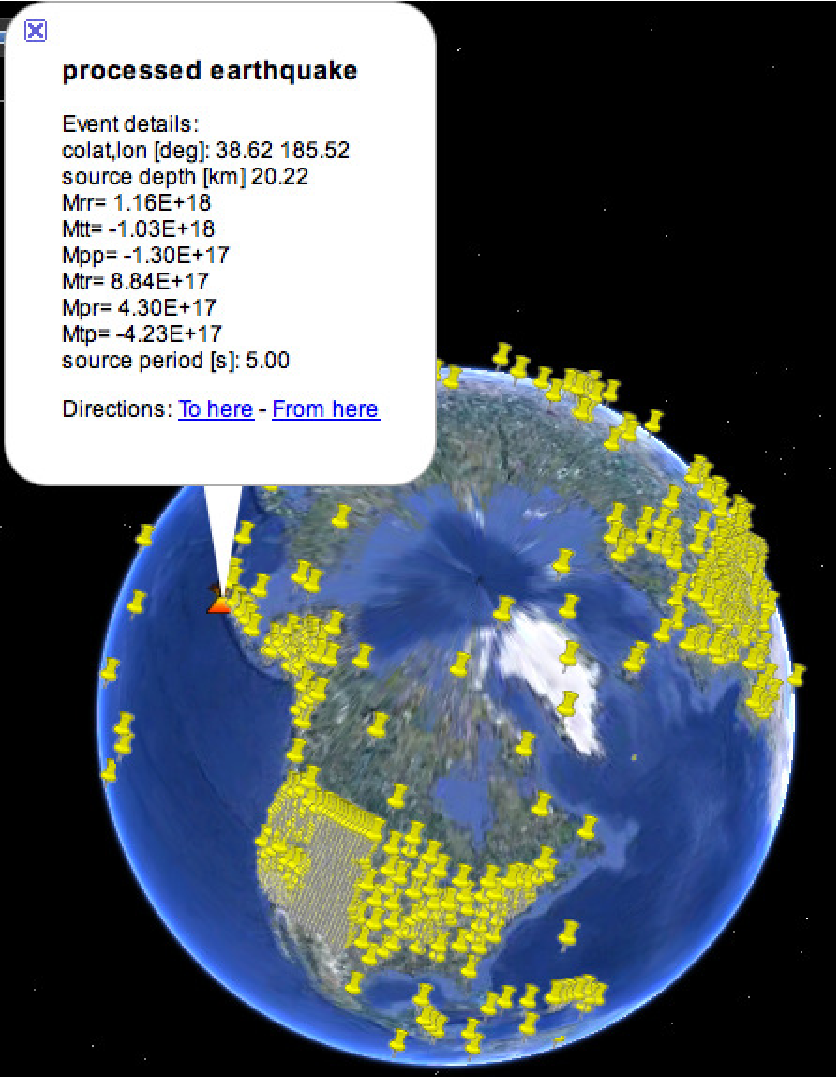
\includegraphics[scale=0.65]{googleearth_src_rec.eps}
\caption{\textit{The kml file output from post processing. It contains the rotated, original source-receiver geometry. Mouse-clicks 
on earthquake location provide source information, mouse-clicks on receiver pins receiver location information and graphics 
of the local seismograms.}}
\end{center}
\end{figure*}

\noindent \textbf{Wavefield snapshots in 3D}.\\
The resultant vtk files are saved into {\tt Data\_Postprocessing/SNAPS/snap*vtk} and can be animated to a movie 
with paraview. Each processor dumps its own file.\\

\noindent \textbf{We have tested:}\\
- rotations from cylindrical to spherical both in the solver and post processing\\
- moment tensor summation to explosion source using moment versus direct inclusion in solver\\
-  compatibility of the two source and receiver file types (including cross-usage)\\
- summation of wavefield snapshots\\
- post processed convolution versus bandlimited stf in solver\\

\noindent \textbf{To Do}:\\
- turn strain wavefields into frequency domain for kerner\\
- rewrite scripts in Python\\
- parallelize snapshot creation\\
- netcdf seismogram databases

\section{Example workflows}
- this is under construction, but in directory EXAMPLES, you'll find
the input files for normal-mode summation code Mineos
(geodynamics.org), against which we have performed some
benchmarks. Caution: We have not managed to create a mode catalog that
is complete, in other words the reference solution is not to be seen
as precise in a quantitative way. Some pdfs in the directory show our
fit. It is useful to re-run such tests when first using AXISEM.

%\newpage
\section{Kernel calculations}
Not included yet at this point... stay tuned!\\

% \noindent The philosophy of this 'scattering-integral' approach to sensitivity kernels 
% is a once-and-for-all calculation of a database for a given background model,
% i.e. including all potential earthquake depths. Everything else related to 
% data, measurements, inversion parameters and observables, time windows, etc 
% is done at the stage of inversion. At this time, output is limited to 
% saving snapshots of the entire 2D mesh or a (contiguous) selection of grid points 
% within elements. Under development is a more 
% sophisticated method to either sample more sparsely, output into a wavelet 
% basis, and straight into frequency domain. 

% In addition to using such sensitivity kernels for inversions, 
% these can be used for Born modeling such that for any given 3D tomographic earth model, 
% it is only a matter of a volumetric integration to determine the seismogram upon such tomographic 
% models. This is not done yet either.

% \subsection{Kerner installation and compilation}
% \subsection{Running the Kerner}
% \subsection{Kerner input}
% \subsection{Kerner computational aspects}
% \subsection{Kerner code structure}
% \subsection{Kerner output}
% \subsection{Kerner post-processing}
% \subsection{Kerner To Do}
\newpage
\section{To Do General}
\subsection{Mesher}
\textbf{Top priority:} Parallelization, 32 processor domain decomposition, netcdf databases\\

\noindent\textbf{Medium priority:} Bending elements for sharp lateral
discontinuities\\

\noindent\textbf{Low priority:} Commenting, cleaning , ellipticity, strongly deformed sphere
(exostars)

\subsection{Solver}
\noindent\textbf{Top priority:} 
\begin{itemize}
\item Attenuation, transverse anisotropy
\item benchmark heterogeneities
\item finite faults, multiple source simulations (4 Mij,
multiple depths, sequential and parallel)
\item dump fields in theta slices, dump fields in frequency domain,
  netcdf, compression
\item Link input to NDLB
\end{itemize}

\noindent\textbf{Medium priority:}
\begin{itemize}
\item Oceans, fluid sphere (surface boundary condition),
  inner-core anisotropy
\item GPU version, local high-order timestepping
\item Incorporate boundary-kernel dumps
\item non-blocking MPI, parallelization benchmark

\end{itemize}

\noindent\textbf{Low priority:}
Gravity, python rewrite of submit.csh

\subsection{Post-processing}
\noindent\textbf{Top priority:} 
\begin{itemize}
\item Benchmark snapshot movies
\item Resampling of timeseries
\item rewrite wavefields in frequency domain
\item finite fault summation
\item extraction from synthetics database (VERCE, IRIS)
\item netcdf, streamline input
\end{itemize}

\noindent\textbf{Medium priority:}
Parallelize snapshot dumps (and other operations)\\

\noindent\textbf{Low priority:} python version

% \subsection{Kerner}
% \noindent\textbf{Top priority:} 
% \begin{itemize}
% \item Quadrature
% \item rotation of kernels from/to actual coordinates
% \item Code efficiency
% \item Benchmarks
% \item misfits
% \item summation for Mij
% \item event-based code (shortcuts for multiple receivers), $G_{ij}$-based code
% \item anisotropy kernels
% \item Link input/output to NDLB
% \item incorporate boundary kernel code
% \end{itemize}

%\noindent\textbf{Medium priority:}
%Born modeling, GPU, On-the-fly kernel generation (fwd wavefield \&
%kernel)\\

%\noindent\textbf{Low priority:}
%Attenuation kernels

%\subsection{Miscellaneous}
%Manual, generation of synthetics database, code release (CIG, VERCE, QUEST)

%\newpage
%\section{Theoretical foundations}
The following sections are excerpts from papers (1)-(4), and not necessarily coherent.

\subsection{Elastodynamic equations of motion: weak form}
For the remainder of this paper, we will treat a non-rotating, 
non-gravitating, isotropic (Lam\'{e} parameters $\lambda$, $\mu$)
earth model. The 3-D elastodynamic weak form comprises the following
three integral equalities for the displacement-potential vector 
$(\bu,\chi)$ in an appropriate space with square-integrable derivatives
for all admissible test or trial functions $(\bw,w)$ \citep{nissen+:07a}:
%
\eqa \label{eq:weak1}
\lefteqn{0=\int_{\rm SIC}\rho\hspace{0.1em}\bw\cdot\ddot{\bu}\,d^3\bx
-\int_{\rm ICB}(\brh\cdot\bw) \ddot{\chi}\,d^2\bx +
}
\nonumber\\
\lefteqn{\hspace{1.5em}
\int_{\rm SIC}\left\{\lambda(\bdel\cdot\bw)
(\bdel\cdot\bu)
+\mu\bdel\bw\!:\!\left[\bdel\bu+\left(\bdel\bu\right)^T\right]\right\}
\,d^3\bx,
}
\ena
%
\eqa \label{eq:weak2}
\lefteqn{0=\int_{\rm FOC}\kappa^{-1}w\hspace{0.1em} \ddot{\chi}\,d^3\bx
+\int_{\rm ICB}w(\brh\cdot\bu)\,d^2\bx -
%}\nonumber\\
%\lefteqn{\hspace{0.5em}
\int_{\rm CMB}w(\brh\cdot\bu)\,d^2\bx
+\int_{\rm FOC}\rho^{-1}\bdel w\cdot\bdel\chi\,d^3\bx,}
\ena
%
\eqa \label{eq:weak3}
\lefteqn{\left\{
\begin{array}{c}
\bph\cdot\bw(r_{\rm r}\hspace{0.1em}\bzh)\delta(t)
\\ \bM:\bdel\bw(r_{\rm s}\hspace{0.1em}\bzh)H(t)
\end{array}\right\}=
%}\nonumber\\ \lefteqn{\hspace{0.5em}
\int_{\rm SMC}\rho\hspace{0.1em}\bw\cdot
\ddot{\bu}\,d^3\bx+\int_{\rm CMB}(\brh\cdot\bw)
\ddot{\chi}\, d^2\bx +}\nonumber\\
\lefteqn{\hspace{11.5em}\int_{\rm SMC}
\left\{\lambda(\bdel\cdot\bw)(\bdel\cdot\bu)
+\mu\bdel\bw\!:\!\left[\bdel\bu+\left(\bdel\bu\right)^T\right]\right\}d^3\bx}
\ena
%
where $\rho$ is the mass density, $\kappa$ the incompressibility, 
$\bph\delta(t)$ the impulsive unity single-force vector acting at the 
receiver at axial radius $r_{\rm r}$ and 
$\bM H(t)$ the moment tensor at the source at axial radius $r_{\rm s}$ as a 
step function in time, and second time derivatives are abbreviated as 
$\ddot{\chi}=\partial^2_t{\chi}$.
The regions solid inner core SIC, fluid outer core FOC, and solid mantle and 
crust SMC in eqs~(\ref{eq:weak1})--(\ref{eq:weak3}) are coupled by virtue of 
the boundary surface integrals over the inner-core (ICB) and core-mantle 
boundary (CMB). The fluid region eq.~(\ref{eq:weak2}) is treated via a 
displacement potential formulation \citep{nissen+:07a}
%
\eq\label{eq:potential}
\bu=\rho^{-1}\bdel\chi,
\en
%
such that the fluid-domain wave equation becomes
\eq\label{eq:fluid_waveequation}
\kappa^{-1}\ddot{\chi}=\bdel\cdot(\rho^{-1}\bdel\chi).
\en
%
Note that the inclusion
of the inverse density in this definition of the potential $\chi$ results in 
boundary integrals in eqs~(\ref{eq:weak1})--(\ref{eq:weak3}) that are 
independent of any intrinsic material properties.
This is slightly different from other spectral-element methods
\citep{KoTr02a,manu04} in which the density-free potential leads
to solid-fluid boundary terms that depend on the discontinuity jumps.
This is necessitated by their inclusion of gravitation, but in our 
non-gravitating case it is indeed feasible to pursue this convenient definition 
in eq.~(\ref{eq:potential}).
For spherically symmetric background models, the 3-D weak system 
eqs~(\ref{eq:weak1})--(\ref{eq:weak3}) may be reduced to its 2-D equivalent 
by factorizing $(\bu,\chi)$ and $(\bw,w)$ into their $(s,z)$ and $\phi$ 
dependencies and analytically evaluating the longitudinal integrals 
such as $\int_0^{2\pi}\sin^2{\phi}\,d\phi=\pi$ as shown by 
\citet[][Section~4.4]{nissen+:07a}.
%
While retaining the $(s,\phi,z)$ cylindrical coordinate
system for the monopole and quadrupole cases, we develop the dipole system 
in the $(+,-,z)$ system, such that
%
\eqa
\lefteqn{u_{\pm}(s,z)=\textstyle{\frac{1}{2}}[u_s(s,z)\pm u_{\phi}(s,z)],}\\
\lefteqn{w_{\pm}(s,z)=\textstyle{\frac{1}{2}}[w_s(s,z)\pm w_{\phi}(s,z)], }
\ena
%
inasmuch as this enables easier implementation of 
the axial boundary conditions given by
\eqa 
\lefteqn{\begin{array}{ll}
\textrm{Monopole:} &
\left(u_s=w_s\right)_{s=0}=0, \label{eq:ax_bc_mo}\\
\textrm{Dipole:}&
\left(u_-=w_-=u_z=w_z\right)_{s=0}=0, \label{eq:ax_bc_di}\\
\textrm{Quadrupole:}&
\left(u_s=w_s=u_\phi=w_\phi=u_z=w_z\right)_{s=0}=0 
\label{eq:ax_bc_qu}.
\end{array}}
\ena
%

\subsection{Meshing}
\begin{figure*}[htb!]
\begin{center}
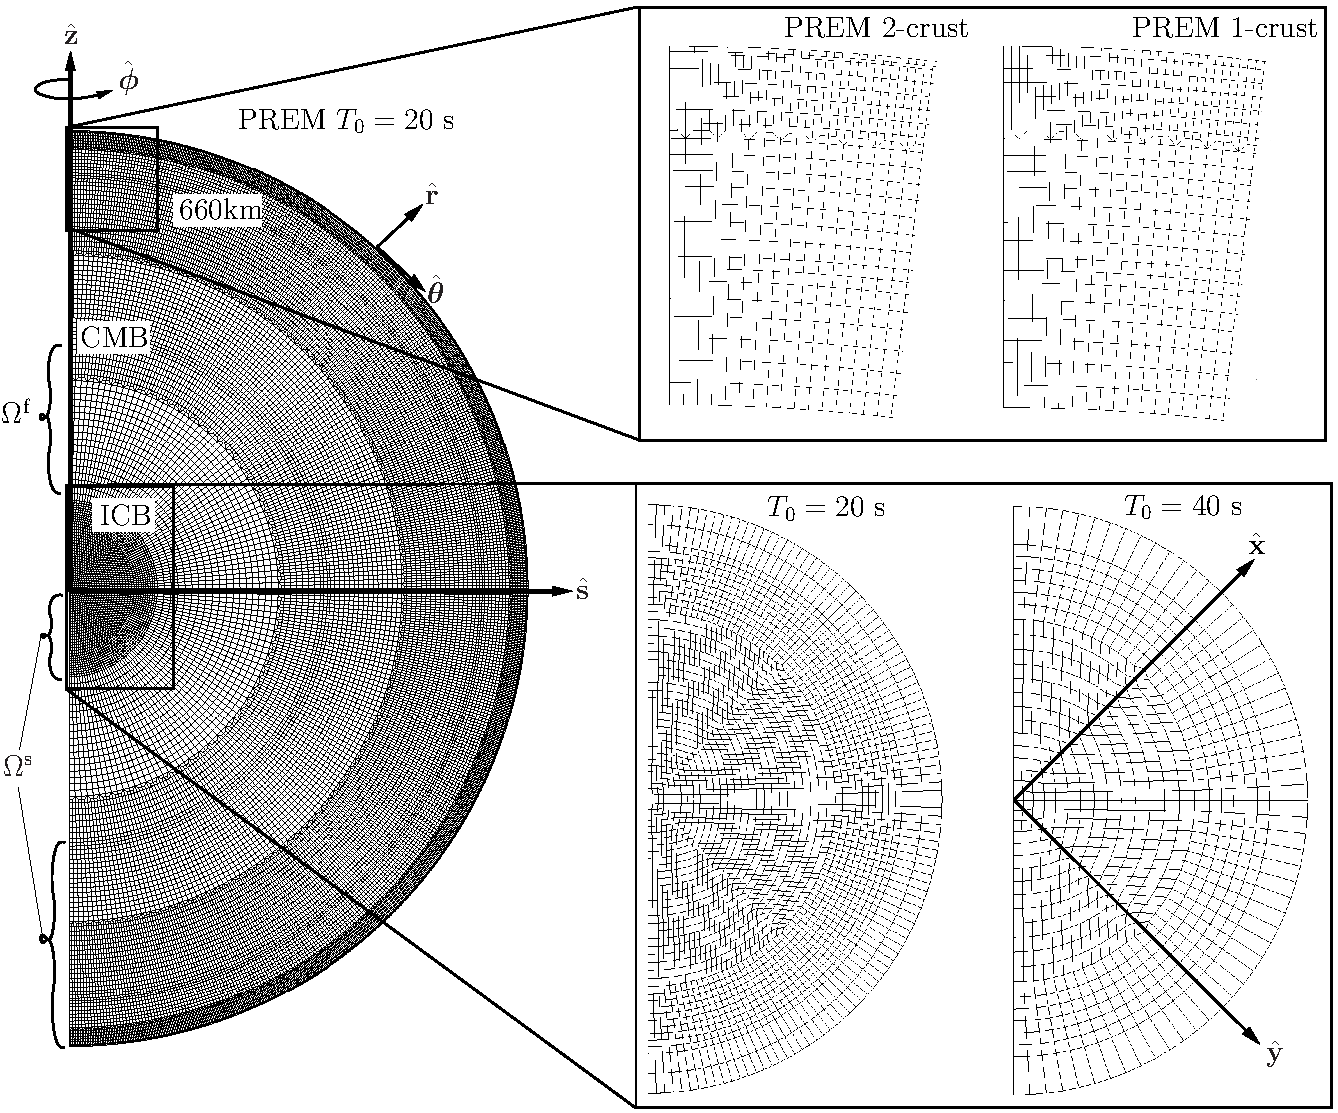
\includegraphics[scale=0.68]{prem_mesh.eps}
\caption{\textbf{Left:} The semicircular, solid-fluid 
domain $\Omega=\Omega^{\rm s} + \Omega^{\rm f}$
discretized for the PREM background model using
quadrilateral elements $\Omega_e$ for dominant source period $T_0=20\, \textrm{s}$.
Note that all discontinuities are honored and several 
conforming coarsening levels are included to maintain a relatively 
constant resolution throughout the domain. 
\textbf{Top right:} Enlargement of the crust for one (right) and two (left) crustal
layers, and the upper mantle, including one mesh coarsening region. 
Note the variable vertical spacing due to discontinuities.
\textbf{Bottom right:} The central region for two resolutions. 
To circumvent the singularity at the center, 
we apply the following analytical expressions to reshape rectangular elements: 
$\left|{x}\right|^p+\left|{y}\right|^p=\left|{r}\right|^p$, 
$x=s+z,\,y=s-z,\,1\le p \le 2$.
This guarantees an easy handle on grid spacing which varies maximally 
at the outermost, deformed elements of this central region and hence 
controls stability and resolution.}
\label{img:prem_mesh}
\end{center}
\end{figure*}

Let us first define some geometric notation. As shown in 
Fig.~\ref{img:prem_mesh} on the left, we work in a semi- disk 
$\Omega=\Omega^{\rm s} + \Omega^{\rm f}$ of outer 
radius $r_0$ spanned by $\bxh^{\rm 2D}=\bsh + \bzh=\brh+\bthetah$,
where $s\in [0,r_0]$, $z\in [-r_0,r_0]$ refer to cylindrical coordinates, and
radius $r\in [0,r_0]$ and colatitude $\theta\in [0,\pi]$ denote the spherical system. 
The longitude $\phi\in [0,2\pi[$ is identical for both coordinate systems, 
$\bxh^{\rm 3D}=\bxh^{\rm 2D}+\bphih$.  Material properties are invariant in 
$\phi$, and the seismic wavefields either invariant (monopole sources) or analytically 
continued from the $(s,z)$ plane \citep{nissen+:07a}; as a result we do not need 
to discretize this third dimension. The grid structure represents the tiling into
non-overlapping solid ($\Omega_e^{\rm s}$) and fluid ($\Omega_e^{\rm f}$) 
elements within which functions are analytically mapped to a reference square
$[-1,+1]^2$ to be expanded upon a polynomial basis 
(see Section~\ref{section:spatial_discretization}).
Fig.~\ref{img:prem_mesh} also depicts magnified regions, showing 
the crust and upper mantle (top right panel) for a two-layered PREM \citep{prem}
crust (left) and a one-layered ``crust'' (right). Note the variable vertical spacing due to the 
discretization of adjacent discontinuities such as $600\,\textrm{km}$ and 
$660\, \textrm{km}$. 

The generation of a tangible mesh is no trivial matter. 
In global seismology, we face the additional complication that the seismic
velocity $v_{\rm p,s}(r)$ generally increases, while horizontal grid spacing
(for spheroidal topologies) decreases with depth which works 
as a doubly detrimental effect for meshing purposes.
Thus, we need to employ mesh coarsening to remediate these issues.
Additionally, a spheroidal grid cannot account for the 
center of the sphere such that one needs to introduce a different (e. g. linear) topology.
The following factors also need to be considered as specific constraints
\citep[see also][Sections~3.1 and 4.1]{nissen+:07b}:
%
\begin{enumerate}
\item Quadrilateral element shapes,
\item Non-overlapping element boundaries,
\item Discontinuities to coincide with element boundaries.
\end{enumerate}
%
Point (i) is a minor issue inasmuch as the nature of 
sharp global boundaries is spherical, i.e. mildly deformed and we do not 
need to accommodate sharp wedges such as in regional velocity models which may
considerably influence the spacing variability and accuracy. Unless the 
expensive mortar element method \citep{manu03} 
or a discontinuous Galerkin approach based on numerical fluxes 
\citep{KaeserDumbser:05} are used, 
constraint (ii) only permits conforming coarsening architectures 
\citep{KoTr02a}, which is what we chose \citep{nissen+:07b}.
Due to the last point (iii), however, we are faced with problems 
such as discretizing the thin crustal layers even for long periods, thus 
introducing local oversampling, or the existence of the fluid outer core, and 
drastic velocity changes across the inner-core boundary 
(see Section~\ref{section:central_region}).
For elastic wave phenomena, one seeks a discretization in which the local
$P$- or $S$-velocity-dependent wavelength $\Lambda(v_{\rm p,s}(r))$ is 
sampled by a minimal variation in the number of grid points per wavelength $n_\Lambda$ 
anywhere in the spatial domain, and, simultaneously, minimal variation 
in the number of time samples $T_0/\Delta{t}$ for the source-induced, 
constant dominant (i.e., peak spectrum) period $T_0=\Lambda(v(r))/v(r)$. 
The limiting values for the number of grid points per 
wavelength, $n_\Lambda^0=\min{\left[n_\Lambda (r,\theta)\right]}$, controlling the 
resolution, and the Courant number, 
${\mathcal C}^0=\max{\left[{\mathcal C}(r,\theta))\right]}$, controlling the stability,
are inherent properties of the numerical scheme.
They are related to $T_0$ and $\Delta t$ via the 
characteristic lead time $\tau_{\rm p,s}(r,\theta)=\Delta x(r,\theta)/v_{\rm p,s}(r)$
\footnote{Subscripts p,s are mnemonic indicators for adhering to the respectively 
largest and smallest velocities for a given location; $\tau_{\rm s}$ in the fluid for example
is obviously defined by the overarching $P$-wave velocity, and near the surface by surface 
wave velocities.}:
%
\eqa 
\lefteqn{T_0 =n_\Lambda^0 \max{\left[\tau_{\rm s}(r,\theta)\right]},} \label{eq:period}\\
\lefteqn{\Delta{t}= {\mathcal C}^0 \min{\left[\tau_{\rm p}(r,\theta)\right]},}\label{eq:timestep}
\ena
%
where for each element, grid spacing $\Delta x(r,\theta)$ also depends on $\theta$ due to the 
irregular Gauss-Lobatto-Legendre point distribution across elements \citep{nissen+:07b}, 
the occurrence of coarsening levels and the linear discretization of the central region.
Meshing in light of these constraints and ideas 
principally aims at simultaneously 
accommodating two factors: 
(i) obtaining a smallest possible total number of elements, i.e. minimizing 
the run-time memory cost with 
(ii) the least variation in $\tau_{\rm p,s}(r,\theta)$. 
This non-unique meshing procedure can be addressed from many angles.
%
\subsubsection{The background-model based spherical mesh}
%
Given the above constraints and the two-dimensional geometry, 
we chose a straightforward approach to define our mesh: 
Given an anticipated dominant period $T_0$ 
to be resolved, the minimal number of grid points per wavelength $n^0_\Lambda$, 
and the location and velocity jump across discontinuities,
we calculate the maximally allowed, smallest global grid spacing  
$\Delta x(\bx_{\rm minx})=T_0/n^0_\Lambda v_{\rm s}(r_{\rm minx})$  for that location 
$\bx_{\rm minx}$ (typically just below the inner-core boundary, or at the surface). 
We determine the exact lowermost radius $r_{\rm sl}$ of the spheroidal domain 
(which characterizes the transition to rectangular element shapes)
by assuming that velocities within the inner core vary very little, starting with 
the grid-spacing constraint $r_{\rm sl}\le r_{\rm minx}$ and moving to 
the next possible lower radius
$r_{\rm sl}=\min\left[r_{\rm icb},{\rm int}\left(r_{\rm minx}/\Delta x(\bx_{\rm minx})\right)\right]$.
Additionally given the number of coarsening levels based 
on the overall change in velocity, and the number of processors $N_{\rm proc}$
(see Section~\ref{section:parallel}), we obtain a permissible number of lateral 
elements at the surface with grid spacing $\Delta x_{\rm lat}(r_0)$ 
upon adjusting $\Delta x(\bx_{\rm minx})$ such that 
$\pi r_0$ is an even multiple of $N_{\rm proc} \Delta x_{\rm lat}(r_0)$.
Progressively moving downwards from the surface while honoring all 
discontinuities and keeping vertical spacing between them similar to 
the ideal value $T_0/n^0_\Lambda \min[v_{\rm s}(r)]$, a coarsening depth 
$\textstyle{r_{\rm c}^i}$ is 
found once $\textstyle{2\tau_{\rm s}(r_{\rm c}^i,\theta)\le T_0/n^0_\Lambda}$, 
i.e. the spacing-velocity combination small enough to double and still resolve $T_0$. 
Once this process is completed, the global time step is found given the limiting 
Courant number ${\mathcal C}^0$ and $\min[\tau_{\rm p}]$ from the newly 
created mesh.
For the SEM, the minimal possible number of points per wavelength is 
$n_\Lambda^0\approx4$ \citep[e.g.][]{Ampuero+:07}, whereas ${\mathcal C}^0$ is 
usually determined empirically and depends on the type and 
order of the time extrapolation scheme (see Section~\ref{section:time_scheme})
and model-space dimension.
We obtain stable, accurate simulations up to ${\mathcal C}^0=0.6$, but one should 
treat this choice carefully for each different mesh and time scheme 
(see Section~\ref{section:time_scheme}). 
Clearly, for any mesh containing model property or grid spacing variations,
these values for $\Delta{t}$ and $T_0$ are the global worst-case combinations, 
and the actual, local Courant number and number of grid points per wavelength are 
variable across the mesh. It is therefore our maxime to construct $\Delta x(r,\theta)$ 
in a way to minimize such variations. All applications in this paper are undertaken 
with a polynomial order $N_{\rm pol}=4$, i.e. having $5$ grid points within an element 
along a given dimension (including its edges); for a more thorough quantification of 
meshing one may however also vary the polynomial order. Note that small polynomial 
orders ease the meshing process in two ways: the smallest grid spacing within elements 
upon a Gauss-Lobatto-Legendre basis varies as $N^{-2}_{\rm pol}$, and, secondly, 
smaller element sizes allow for easier adaptation to material interfaces, especially 
regarding closely spaced discontinuities like in the crust.
Fig.~\ref{img:prem_mesh} shows an example of a PREM model discretization using 
this method for $T_0=20 \, \textrm{s}$ (left), and two magnified regions of interest, i.e. 
the crust and upper mantle (top right) and the central region 
(bottom right, see next section). Clearly, lower resolutions (being confronted with 
the same background model as higher resolution realizations), are 
less effective and expose larger spacing variations, as seen in the crust. 
It is noteworthy to highlight that meshing is done only upon the lowest velocities
(surface waves near the surface, $S$ waves in deeper solid, $P$ waves in fluid), but one
subsequently determines the time step (i.e. the other component of the cost of the 
scheme besides the number of elements ) based on largest ($P$ wave) velocities. 

\begin{figure*}[t!]
\begin{center}
\includegraphics[scale=0.7]
{char_times_fig.eps}
\caption{Elementally minimal and maximal characteristic lead times scaled by 
the time step and Courant number, 
$\tau_{\rm p,s} {\mathcal C}^0/\Delta{t}$ in the spherical part of the model space as  
a function of radius.
We depict PREM meshes for source periods $T_0=10\,\textrm{s}$ (left) and 
$T_0=20\, \textrm{s}$ (right). The vertical line to the left 
denotes unity, i.e. minimal possible $\min[\tau_{\rm p}]$ due to the definition of $\Delta{t}$ in 
eq.~(\ref{eq:timestep}), and the vertical line to the right the corresponding maximal 
value given by the relationship for the source period, eq.~(\ref{eq:period}), i.e. 
$T_0 {\mathcal C}^0/(n^0_{\Lambda}\Delta{t})$.}
\label{img:char_time}
\end{center}
\end{figure*}
%
It is thus desirable to at least assess this entirely non-unique, potentially iterative process 
a posteriori in terms of efficiency and overall cost. 
In the interest of generality, we present examples of different mesh 
realizations in terms of non-dimensionalized parameters, namely the 
characteristic lead time 
%
\eq
\frac{\tau_{\rm p,s}}{\min[\tau_{\rm p}]}=\tau_{\rm p,s}\frac{{\mathcal C^0}}{\Delta{t}},
\en
%
and the local oversampling ratio
%
\eq
\frac{T_0}{\Delta{t}^{\rm eff}(\bx)}=\frac{T_0}{n_\Lambda^0\tau_{\rm p}(\bx)}.
\en
%
\begin{table*}[htb!]
\begin{center}
\caption{Characteristic lead times and time steps for various mesh resolutions and Courant 
number ${\mathcal C}^0=0.6$ and $n_\Lambda^0=6$.}
\label{table:char_time} 
\begin{tabular}{@{}cccccccc}
\hline\hline
$T_0\, [s]$ & $\min{\left(\tau_{\rm p}^{\rm lat} \right)}\,[{\rm s}]$ &  
$\min{\left(\tau_{\rm p}^{\rm rad} \right)}\,[{\rm s}]$ &
$\max{\left(\tau_{\rm s}^{\rm lat} \right)}\,[{\rm s}]$ & 
%$\max{\left(\tau_{\rm s}^{\rm rad} \right)}\,[{\rm s}]$ & 
$\Delta t\,[{\rm s}]$ &  $\max{\left(\tau_{\rm s} \right)} {\mathcal C}^0/\Delta t$ & 
$T_0/\min\left(\Delta t^{\rm eff} \right)$
\\
\hline\\
$5$   & 0.0917& 0.117 & 0.832 & 0.0555 & 9.08 & 8.99 \\[10pt]
$10$ & 0.182 & 0.234 & 1.66 & 0.111 & 8.97 & 9.16 \\[10pt]
$20$ & 0.356 & 0.239 & 3.32 & 0.121 & 16.46 & 13.9 \\[10pt]
$40$ & 0.687 & 0.239 & 6.45 & 0.121 & 32.0 & 27.9 \\[10pt]
%
\hline
\end{tabular}
\end{center}
\end{table*}
%
In both cases, the definition contains all relevant constant parameters such that 
this analysis can be viewed as independent both of the actual mesh resolution and the 
choice of the spatio-temporal discretization scheme (spectral elements, 
finite differences etc.) and may therefore be
useful in estimating the mesh quality for varying resolutions and methods.
In Fig.~\ref{img:char_time}, we show the variation of the non-dimensional 
characteristic lead time for the spherical part 
of the domain as a function of radius. The panels are for different 
PREM model realizations with $T_0=10\, \textrm{s}$ on the left and
 $T_0=20\, \textrm{s}$ on the right. 
For each mesh, we plot radial/lateral and maximal/minimal values of 
$\tau_{\rm p,s}$ for each element, respectively.
Clearly, the mesh coarsening is reflected by the jumps in lateral spacing, whereas 
the radial structure is smoothly kept within the bounds set by the lateral values. 
Another apparent feature is the fact that the lateral characteristic lead times 
$\tau_{\rm p}$ seem to follow two profiles, i.e. for a given radius, there are 
two minimal spacings. This is merely the result of the fact that we employ 
a different polynomial basis within axial elements 
(Gauss-Lobatto-Jacobi (GLJ) points) than for non-axial elements 
(Gauss-Lobatto-Legendre (GLL) points): The profile with 
smaller values is due to axial elements, and all others follow the profile for 
larger values \citep[see][Section~3]{nissen+:07b}. Note also that the distinction 
only exists for lateral $\tau$ as we utilize the same Gauss-Lobatto-Legendre 
points in the radial direction for all axial and non-axial elements. The difference 
in largest elemental spacing within $\tau_{\rm s}$ is much smaller between GLJ and 
GLL, but still visible in Fig.~\ref{img:char_time}. 
Otherwise, the distribution of lead times is similar in both cases, suggesting that 
the meshing process is consistent and independent of the actual resolution.
Adhering to the non-dimensional nature of the function, it is also curious to note that 
we are faced with a variation of less than an order of magnitude
for the characteristic lead time in the $10\,{\rm s}$ case, but a  
doubled variation for $T_0=20\, \textrm{s}$ due to the fact that the 
crustal layer thicknesses at such low frequencies 
determine the smallest spacing rather than the resolution. Table~\ref{table:char_time} illuminates
this issue in a quantitative way by listing the characteristic lead times for meshes 
between $T_0=5\,{\rm s}$ and $T_0=40\,{\rm s}$. Evidently, the smallest radial spacing 
is constant for meshes above $10\,{\rm s}$ such that the time step does not increase with the
period, and the above-mentioned ratio of minimal versus maximal $\tau$ increases with the 
period. Apart from these cases of $T_0>10\,{\rm s}$, 
the meshing process is consistent and independent of the resolution in that
source period $T_0$ and $\tau$ are linearly related and their ratio constant.

\begin{figure}[htb!]
\begin{center}
\includegraphics[scale=0.55]
{prem_10sec_coars3_oversampling_rad_el.eps}
\caption{Local temporal oversampling in terms of period and time step for the mesh down to 
$10\, \textrm{s}$. Unity would be equivalent to the ideal case 
of no variation for 
the characteristic lead time $\tau$ whatsoever, impossible for any elastic medium.
A more realistic aim, the empty circles to the left depict the ratio $\tau_{\rm p}/\tau_{\rm s}$ which 
represents the limiting case of ideal meshing for the given background model \textit{and} the 
inevitable grid spacing variation due to the polynomial basis of Gauss-Lobatto-Legendre points
\citep{nissen+:07b}, i.e. with no oversampling due to suboptimal meshing.
The vertical line to the right 
is the constant ratio $(T_0/\Delta{t})({\mathcal C}^0/n^0_\Lambda)$, i.e. the global worst case scenario 
after which these parameters have been chosen. }
\label{img:spacing_ratios}
\end{center}
\end{figure}
%
Fig.~\ref{img:spacing_ratios} is an additional characteristic for the mesh 
efficiency, painting its local oversampling ratio as a function of
radius. This function essentially denotes the local numerical gap between 
defining grid spacing upon the period and largest possible spacing, 
but simultaneously noting the smallest spacing to abide stability for the temporal 
extrapolation. The lower bound is the mere $\tau_{\rm p}/\tau_{\rm s}$ ratio, 
i.e. the ideal case with local oversampling due to meshing, and the higher bound is 
the scaled ratio of period and time step $T_0/\Delta{t}$, i.e. the global worst case.
As before, the radial spacing follows a relatively smooth profile along the idealized 
case of the characteristic lead time ratio, whereas the lateral spacing is subject to
coarsening layers and the main contributor to spacing variability or deviation 
from the smooth profile. Table~\ref{table:char_time} lists this oversampling 
ratio in the last column for different resolutions. Similar to the characteristic 
lead time, the non-dimensionalized oversampling is constant and independent 
of the actual resolution once discontinuity locations do not determine the 
grid spacing as for $T_0>10\,{\rm s}$.
Again, it  may be interesting to conduct a thorough 
comparison of these functions for a variety of background models and numerical 
methods. In our case, it is verified that the meshing process is consistent for 
varying resolutions and optimally discretized where possible.
Both these latter plots give an idea about the mesh quality, inasmuch as they 
generally delineate excursions from the idealized respective minimal values 
\citep[compare][]{KoTr02a}. We shall take this to the next level of estimating 
a non-dimensionalized, global mesh cost after the next section on the central region.
%
\subsubsection{The central region}\label{section:central_region}
%
The singularity at $r=0$ is circumvented by rectangular element discretization
\citep{manuthesis} which introduces an additional problem, namely the vast 
spacing variations between the rectangular $r<r_{\rm sl}$ 
and circular regions $r>r_{\rm sl}$. We accommodate this by defining 
(see Fig.~\ref{img:prem_mesh})
%
\eq \label{eq:central}
\left|{x}\right|^p+\left|{y}\right|^p=\left|{r}\right|^p,\; 
x=s+z,\,y=s-z,\,1\le p \le 2.
\en
%
where the exponent $p$ can vary either linearly, quadratically, or cubically 
with the radius $r$. We thereby maintain an acceptable
$\min{[\tau_{\rm p}]}\le\tau_{\rm p,s}(r<r_{\rm sl},\theta)\le\max{[\tau_{\rm s}]}$ 
where we take the extremal values of $\tau_{\rm p,s}$ from the spherical 
domain $r\ge r_{\rm sl}$, thereby avoiding the case that these linear elements
determine the overall cost. 
Applying the mapping eq.~(\ref{eq:central}), elements along the 
diagonal directions $x=0$ and $y=0$ are extremely deformed, and therefore 
subsequently stretched outwards by half an element size, respectively 
(see Fig.~\ref{img:prem_mesh} c).
The high mesh density in the inner core stems from the fact that we effectively follow
a drastic velocity drop across the inner-core boundary since we only need to resolve
outer-core $P$ waves but inner-core $S$ waves.
Fig.~\ref{img:central} illustrates the central region in terms of relative points 
per wavelength (left) $n_{\Lambda}(\bx)/n^0_\Lambda$, and local oversampling 
(right) $T_0/(\tau_{\rm p}(\bx) n^0_\Lambda)$ as (interpolated) 2-D functions across 
the central region. The colorbars respectively range from the minimal to 
the maximal values of the spherical domain, which is taken as the 
goal to stay within. In both critical cases, our approach to minimize element 
distortion via eq.~(\ref{eq:central}) seems to be verified in that all elements in 
this region maintain characteristic lead times within the bounds of the 
spherical domain and thus do not further deteriorate the overall trade-off 
between $T_0$, total number of elements, and $\Delta t$.
%
\begin{figure}[tb!]
\begin{center}
\includegraphics[scale=0.6]
{prem_10sec_coars3_centralregion_period_dt_per_over_dt.eps}
\caption{Numerical parameters in the central region for the PREM mesh down to 
$10\, {\rm s}$. \textbf{Left:} Number of points per 
$S$ wavelength scaled by the minimal value $n_\Lambda^0=4$. The fact that we need to resolve 
$S$ waves in the inner core as opposed to outer core results in a drastic minimal velocity drop across 
the ICB and accordingly grid densification. \textbf{Right:}  Local oversampling ratio, 
i.e. the period $T_0$ versus characteristic lead spacing time $\tau_{\rm p}$. 
The colorbar bounds represent the extremal characteristic lead times in the spherical domain above.}
\label{img:central}
\end{center}
\end{figure}
%
\subsubsection{Mesh scaling and computational cost}
%
Based on the two previous sections, we now revert to estimating the overall 
cost of the scheme that is launched upon a mesh as defined here. 
In a recent study, \citet{Ampuero+:07} suggest for the cost
${\$\$}$ on a topologically and structurally homogeneous mesh the 
compact relationship
%
\eq\label{eq:abscost_homo}
\lefteqn{{\$\$} =  E(N_{\rm pol}) \left(\frac{L}{h}\right)^D \frac{L/v}{\Delta t},}
\en
%
where $E(N_{\rm pol})$ denotes the number of floating-point multiplications per element 
as a function of polynomial order $N_{\rm pol}$, $L$ is the total propagation length, 
and $D$ the dimension.
Assessing our highly non-regular mesh, we modify this expression into
the generalized, non-dimensional philosophy such that we can 
determine the quality and scaling properties as a function of the resolution, 
also bypassing $E(N_{\rm pol})$ since we keep $N_{\rm pol}$ fixed in this 
analysis for different meshes.
Let the cost $\$\$={\mathcal I}{\mathcal E}$ be factorized into
instantaneous cost (or an indicator for run-time memory occupation)
${\mathcal I}$ formed by the total number of elements $N_{\rm el}$ in the mesh, 
and secondly the evolving/extrapolation cost ${\mathcal E}$, 
i.e. the number of time steps:
%
\eqa
\lefteqn{{\mathcal I}=\frac{N_{\rm el}}{N_{\rm el}^{\rm ref}}=
\frac{2}{\pi r_0^2} (N_{\rm pol}\Delta x_{\rm max})^2 
N_{\rm el} ,} \label{eq:instcost}\\
\lefteqn{{\mathcal E}=\frac{\Delta{t}^{\rm ref}}{\Delta{t}}=\frac{T_0}{2\Delta{t} } . }
\label{eq:extrapolcost}%\\
\ena
%
In eq.~(\ref{eq:instcost}), we scale the total number of elements $N_{\rm el}$ with an approximate 
reference number of fewest possible elements, 
i.e. assuming global coverage via the largest grid spacing, such that $\min[{\mathcal I}]=1$ 
represents the idealized scenario were there no velocity and spacing variation for a given period $T_0$. 
In eq.~(\ref{eq:extrapolcost}), we take the idealized sampling rate from the Nyquist sampling 
theorem as $\Delta{t}^{\rm ref}=T_0/2$, such that again $\min[{\mathcal E}]=1$ represents the 
cheapest possible setting. In this scale-invariant formulation, we forego the inclusion of the total 
simulation length $L/v$ as in eq.~(\ref{eq:abscost_homo}) since this would simply result in the 
same multiplicative factor for all cases.
%
\begin{figure}[tb!]
\begin{center}
\includegraphics[scale=0.66]{cost_fig.eps}
\caption{Computational cost of the mesh. \textbf{Left:} Instantaneous cost, i.e. the 
size of the mesh. \textbf{Right:} Extrapolation cost, i.e. the number of time steps. 
Both functions are constructed in a non-dimensionalized fashion
such that they cancel out resolution dependencies when 
plotted as a function of the source period $T_0$.}
\label{img:cost}
\end{center}
\end{figure}
%
In contrast to \cite{Ampuero+:07}, we also refrain from computing a multiplicative total cost 
since the actual non-dimensionalized values of the two respective definitions 
eqs~(\ref{eq:instcost})--(\ref{eq:extrapolcost}) 
bear no interconnection, especially with regard to large values.
It is nevertheless noteworthy that the overall decisive factor for the cost of a given mesh 
for $T_0$ turns out as $N_{\rm pol}^2 \Delta x_{\rm max}^2 N_{\rm el}/\Delta{t}$.
Also note that the respective dependence on the period  (via $\Delta x_{\rm max}$ in eq.~(\ref{eq:instcost})) 
counteracts  the 
expected dependence of the 2-D spatial and 1-D temporal discretization such that the actual 
cost as defined in eqs~(\ref{eq:instcost})--(\ref{eq:extrapolcost}) 
is independent of the resolution itself by virtue of the chosen normalization. 
Fig.~\ref{img:cost} depicts the instantaneous and 
extrapolation cost, respectively, as a function of period for PREM and PREM-1-crust 
realizations of the mesh strategy described in the previous sections. 
Evidently, low resolution is relatively ineffective inasmuch as the time step is controlled 
by the smallest grid spacing which in turn is the mere radial separation of the two closest 
discontinuities, mostly in the crust. For both cost functions, we enter another regime below 
$10\,\textrm{s}$ , where the meshing process itself controls the computational cost and the 
two models are equally expensive. 
The slight increase of instantaneous cost with higher resolution below $7\,\textrm{s}$ 
represents the cutoff resolution below which the instantaneous cost does not decrease 
any further due to the background model heterogeneities, overall velocity 
contrasts and the associated necessity to honor smaller velocities with smaller 
element sizes, independent from the actual resolution.
The seemingly asymptotic convergence  to $50$ for the extrapolation cost reflects 
the ratio $T_0/\Delta t$ as shown in Fig.~\ref{img:spacing_ratios} which is then 
independent of the resolution but merely the difference in maximal and minimal 
characteristic lead times. In both instantaneous and extrapolating cost functions, 
the mesh is more cost-effective with increasing resolution, which is 
expected as we asymptotically mimic a continuous medium 
when increasing resolution at fixed background structure: We are progressively 
less limited by grid constraints such as discontinuity locations, permissible lateral 
number of elements due to the number of processors, coarsening levels, and 
hemispheric mirror symmetry as will be further elucidated in the next section.
%
\begin{figure*}[tb!]
\begin{center}
\includegraphics[scale=0.54]{dd_fig.eps}
\caption{Domain decomposition for $T_0=10\,{\rm s}$ 
and four (left), eight (middle), and sixteen (right two panels) processors.
Note that each processor has the same number of elements 
(``efficiency''), and maximally two neighbors (minimal latency)
with small shared boundaries (i.e., small bandwidth). 
Each processor touches the axis, albeit to varying amounts. Axial terms 
are however 1-D, and as such do not add any countable CPU time to the 
overall scheme.The central region is subdivided such that each processor 
has exactly the same amount of elements.}
\label{img:dd}
\end{center}
\end{figure*}
%
\subsubsection{Parallelization and domain decomposition} \label{section:parallel}
%
The meshes described in the previous section, even though only 2-D, are dense enough 
to reach typical memory limits when going below $T_0\sim 5 \, \textrm{s}$: 
The mesh at $5\,\textrm{s}$ contains about $10^7$ grid points, 
each carrying up to $40$ (single-precision) global, scalar floating-point 
numbers at run-time memory, summing up to $1.5\, \textrm{GByte}$ shared memory.
This shall not remain a centennial problem in the wake of hardware improvements, 
but as we do strive to compute kernels down to $1\, \textrm{s}$, it is indispensible 
to parallelize the method, especially in light of the extensive wavefield output.
With the potentially limited life-time of the parallelized version in mind and the fact 
that one may compute synthetics and kernels for lower resolutions, 
the code is written in a parallel modular way such that all message passing, 
communication and domain decomposition issues are confined to 
a single module and moderate amount of call statements hence it being trivial 
to denounce the parallel world and adopt the method for entirely serial simulations.
When spreading the computational workload across several separate CPUs and 
memory units, one seeks to minimize \textit{inefficiency} (work imbalance), 
\textit{latency} (number of neighboring processors) and \textit{bandwidth} 
(vector length to be communicated). We follow an approach based on global 
numbering \citep{TufoFischer:01,dfm}, predefining one index vector of 
arbitrarily located grid points for each processor-processor pair to be 
exchanged such that processors may harbor separate subdomains or share 
multiple edges but always exchange one message with any neighbor. 
This flexibility enables us to e.g. let each CPU belabor fluid {\it and} solid regions, 
hence reducing imbalance.
%
Fig.~\ref{img:dd} shows examples of our domain decomposition strategy 
for the mesh down to $T_0=10\,{\rm s}$ for four, eight, and sixteen 
processors from left to right: 
We chose to split the domain laterally such that each processor has an 
equal amount of fluid and solid elements at the generally inevitable expense of 
focusing the axial workload (additional terms and source) onto two 
processors that occupy most of the axis (e.g. black and green domains in the 
left panel). 
%
As will be seen, this shall not hamper the favorable scaling of 
our parallelization. At this point, it is important to recall our application of 
saving spatio-temporal wavefields for the computation of sensitivity kernels, 
i.e. such extensive I/O shall overshadow any slight processor imbalance due to
additional axial terms or the source by and large. 
The actual number of processors needs to be an even 
multiplicative of $2$ due to the equatorial symmetry and the connection
of the spheroidal with the central region. While the former is trivial to 
decompose simply based upon colatitude, the latter central part poses 
a problem in keeping with the load-balance philosophy.
%
\begin{figure}[tb!]
\begin{center}
\includegraphics[scale=0.4]{parallelscaling_both_2.eps}
\caption{Relative simulation times of the time loop for different numbers of processors 
$N_{\rm proc}$, either keeping the total memory (i.e., constant mesh and resolution) 
or the per-processor memory constant (i.e., constant job load per processor). $t_0$ 
is the CPU time for the one-processor case;
the diagonal constitutes the case for which CPU times are unaffected by the parallelization. 
In both our cases, the parallelization 
plays such a minor role that simulation times are actually \textit{shorter} for more processors, 
adhering to smaller memory occupation and negligible parallel communication patterns.} 
\label{img:scaling}
\end{center}
\end{figure}
%
We tackled this issue as seen in the magnified panel on the right of 
Fig.~\ref{img:dd} by defining discrete polynomials $z(s)$ up to 
second order for each processor's central region under the premises of 
covering the same discrete area, maintaining a respective 
vertical and diagonal ``thickness'' of at least one element,
choosing outer end locations given by the 
spheroidal processor latitudes, and touching the axis with at least one 
element. During this elemental fitting to the polynomial, 
we ``fix'' non-smooth processor boundaries including those that 
develop elemental plateaus and corners.
%
Nevertheless, this procedure carries with its iterative, element-by-element 
search some inevitable, unaesthetic remnants such as the spikes in the processor 
boundary shapes, but such negligible deviations from the same-surface ideal 
seem inevitable when working with such domains.  
Most importantly, this approach guarantees exact load balancing in terms of 
number of elements, and minimal communication such that each processor only 
touches maximally two neighbors, taking an inherent topological 
advantage of our 2-D semi-disk bounded by the axis. 
%
%
Again, we strive to quantify this parallelization approach in a 
relative, non-dimensional sense. Two end-members are considered, 
namely the fixation of total and processor-specific memory. 
Keeping the total memory constant means that the code ideally speeds up 
by the factor $N_{\rm proc}$, whereas constant memory per processor means 
that for constant run-time, the resolution should accordingly 
increase with $N_{\rm proc}$. Fig.~\ref{img:scaling} shows some results from 
simulations up to $16$ processors: In both end-member cases, the curves lie 
below the diagonal which is the communication-blind scaling where CPU times 
are inversely proportional to $N_{\rm proc}$, such that our parallelization is 
actually favorable: The total CPU time of a parallel job is \textit{smaller} than 
the according CPU time of the single-processor job. This result is mainly attributed 
to the memory occupation, but more importantly, validates our domain decomposition 
and parallelization scheme as completely transparent to the CPU times. Generally though, 
minute hardware and network fluctuations between different nodes may have well affected
these CPU times such that the actual values shall be viewed with caution. Clearly, though, 
this is an extremely favorable result, and shall be repeated in a thorough benchmark 
on different architectures in the future.  
%
Finally, Fig.~\ref{img:message_surf_vol} depicts another quality control on the
domain decomposition for varying resolutions: We plot the sum of message
interfaces (counted in unique grid points) versus the number of unique grid
points of the entire domain as a function of $N_{\rm proc}$, in other
words describing the fractional spatial size of messages related to the total mesh. 
For all feasible cases of up to $32$ processors (extrapolating this function), 
we retain moderate, sub-percentile values such that CPU times shall not be 
significantly affected by the mere size of messages.
If one however extrapolated these to very large numbers of processors (beyond $32$), 
it may be worthwhile to consider other domain decomposition strategies 
which keep these ratios smaller (e.g. 2-D decomposition).
See Appendix~\ref{appsection:runtime_breakdown}
for more on fractional runtimes and parallel scaling.
%
\begin{figure}[t!]
\begin{center}
\includegraphics[scale=0.4]{sum_messages_surf_vol.eps}
\caption{The sum over all message sizes versus total volume size 
(both counted in unique grid points) for each mesh and $N_{\rm proc}$, 
i.e. the grid fraction that communicates. 
If this function reaches a significantly large value, then the 
parallelization and message passing will take up larger fractions 
of the CPU time, but as our case indicates, it shall asymptotically 
approach value below $1\,\%$ for all projected, feasible cases of 
up to $32$ processors. }
\label{img:message_surf_vol}
\end{center}
\end{figure}
%
%
\subsection{Spectral-element discretization}
In this section, we give a brief overview of the aspects of the 
spectral-element method (SEM) that are relevant for the discretization, 
which we take up in the following sections. 
The reader is referred to the detailed literature
for a full description of the approach, e.g. \citet{dfm} and 
\citet{karniadakis} 
on the mathematical foundations of the SEM with a focus on fluid dynamics; 
\citet{KoVi98}, \citet{KoTr99}, \citet{KoTr02a}, \citet{manu03}, and 
\citet{Chaljub+:06} on the 
elastodynamic SEM; and \citet{bernardi} and \citet{fournier04} on 
discretizing an axisymmetric system.
%
%
\begin{figure}[htb!]
\begin{center}
\includegraphics[scale=0.8]{fig1.eps}
\caption{The mesh architecture. The geometric mapping mentioned in 
Section~\ref{section:geometrical} transforms the unit square element (A), 
within which all computations are undertaken, into any quadrilateral element 
$\Omega_e$ or $\bar{\Omega}_e$ (B). (C) shows the actual mesh used 
in the simulations described in Section~\ref{section:validation}. 
Three different element geometries, as defined in 
Appendix~\ref{appsection:geom_mapping} and 
Fig.~\ref{figa1}, are used to construct this mesh such that spacing 
variations are kept small. The radius of the earth is $r_0$, and 
the left straight edge is the non-physical axis of 
symmetry for which we employ different discretization rules due to the 
appearance of singularities $s^{-1}$.}
\label{fig1}
\end{center}
\end{figure}
%
\subsubsection{Geometrical mapping and discretization}\label{section:geometrical}
%
As in any element-based method, we discretize and decompose the continuous, 
open domain $\Omega$ with boundary $\partial\Omega$ 
into a union of non-overlapping elements. 
For clarity, we shall distinguish the so-called axial elements, which share an 
edge with the axis of symmetry $s=0$, from the remaining ones. Any axial 
element is then denoted by $\bar{\Omega}_{e}$, $e=1,...,\bar{n}$, 
while a non-axial element is represented by $\Omega_e$, $e=1,...,n$, such that 
the total number of elements forming the skeleton of the spectral-element 
mesh is $n+\bar{n}$.
Throughout the paper, we will consistently utilize an overbar to 
identify axial quantities. This decomposition permits us to break any global 
integration over $\Omega$ up into $n+\bar{n}$ local integrations, each 
spanning their respective elements, such that we define all integrands on 
the elemental level and only connect these to the global system when 
marching forward in time, as detailed in 
Section~\ref{section:discr_eq_motion}. 
In the 2-D spectral-element discretization used here, we confine $\Omega_e$ or 
$\bar{\Omega}_{e}$ to be a quadrilateral image of a reference square 
spanning $-1\le\xi\le 1$, $-1\le\eta\le 1$, defined by the invertible 
mapping $s=s(\xi,\eta)$, $z=z(\xi,\eta)$ (Fig.~\ref{fig1}~(A),~(B)). 
The exclusion of other geometries 
such as triangular elements will not hamper the feasibility of our approach 
given the spherical nature of spherical-earth discontinuities, i.e., the 
mildly deformed elemental shape. 
The D-shaped, planar domain with radius $r_0$ is shown in Fig.~\ref{fig1}~(C),
along with the mesh discretization as used throughout this paper.
Note that we included several conforming coarsening levels to 
reduce grid spacing variations \citep{KoTr02a} which generally trade 
off the time step (depending on the minimal spacing) with the frequency 
resolution (depending on the maximal spacing) in any numerical scheme. 
The center is discretized using rectangular elements \citep{manuthesis}.
The expression of the mapping depends on the elemental shape and is
either analytical or subparametric \citep{fournier04}. Explicit formulae and 
illustrations are given in Appendix~\ref{appsection:geom_mapping}.
With a given element shape, we can then compute the elemental Jacobian
\eq \label{eq:jacob}
{\mathcal J}(\xi,\eta)=
\frac{\partial(s,z)}{\partial(\xi,\eta)}=
\det\left(\begin{array}{cc}
\partial_\xi s & \partial_\eta s \\
\partial_\xi z & \partial_\eta z
\end{array}\right).
\en
%
Derivatives $\partial_s$ and $\partial_z$ of a function 
$u(s(\xi,\eta),z(\xi,\eta))$ map into the reference square as
\eq \label{eq:ds_u}
\partial_{s}u(s,z)=
\left[\partial_{\eta}z(\xi,\eta)\partial_{\xi}u(s(\xi,\eta),z(\xi,\eta))-
\partial_{\xi}z(\xi,\eta)\partial_{\eta}u(s(\xi,\eta),z(\xi,\eta))\right]
{\mathcal J}^{-1}(\xi,\eta),
\en
%
\eq \label{eq:dz_u}
\partial_{z}u(s,z)=
\left[-\partial_{\eta}s(\xi,\eta)\partial_{\xi}u(s(\xi,\eta),z(\xi,\eta))+
\partial_{\xi}s(\xi,\eta)\partial_{\eta}u(s(\xi,\eta),z(\xi,\eta)) \right]
{\mathcal J}^{-1}(\xi,\eta).
\en
%
Elements $\bar{\Omega}_{e}$ adjacent to the non-physical boundary $s=0$ 
(i.e., the axis of symmetry) are treated separately to accommodate 
singularities arising from terms 
involving $s^{-1}$ in the equations of motion (\ref{monosmc})--(\ref{quadsmc}).
We describe the treatment of the non-axial elements in 
Section~\ref{section:nonax} and briefly discuss the additional complexities 
for the axial elements in Section~\ref{section:ax}.
%
%
\subsubsection{General non-axial functional discretization}\label{section:nonax}
%
The spectral-element approach presented here relies on quadrature of the 
Gauss-Lobatto type, allowing us to enforce continuity across element 
boundaries conveniently by including the nodes $\xi=-1,1$. 
$N$th order Legendre polynomials $P_N$ 
(see Appendix~\ref{appsection:sem_lib}, eq.~(\ref{appeq:legendrepol})) 
are then invoked to define the most accurate and natural quadrature rule 
\citep{dfm}. Quadrature nodes are hereupon defined as the zeroes of 
$(1-\xi^2)\partial_\xi P_N(\xi)$, 
denoted as Gauss-Lobatto-Legendre (GLL) points $\xi_p,\;0\le p \le N$.
To interpolate functions upon these GLL nodes, we introduce Lagrange 
interpolating functions $l^N_i(\xi_p)$ of polynomial order $N$, 
$0\le i,p\le N$, such that: $l^N_i(\xi_p)=\delta_{ip}$ (see 
Appendix~\ref{appsection:gll}). For clarity, we shall denote GLL nodes 
in the $\xi$ direction as $\xi_i$ and in the $\eta$ direction as $\eta_j$.
The choice of Lagrangian interpolation upon GLL nodes yields the desirable 
property of a diagonal mass matrix, thereby greatly reducing the effort on 
time marching (see Section~\ref{section:discr_eq_motion}).
Furthermore, the orthogonality of coordinates $\xi$ and $\eta$ in a 
quadrilateral element geometry allows for separation of variables and 
leads to efficiently implemented tensor products (see 
Appendix~\ref{appsection:stiffness_mxm}).
Elemental integrals over $(s,z)$ may now be mapped into $(\xi,\eta)$ and 
discretized as
%
\eqa \label{eq:gll_quad_nonax}
\lefteqn{\int_{\Omega_e}u\left(s,z,t\right)s\,ds\,dz
=\int_{-1}^{1}\int_{-1}^{1}u\left(s(\xi,\eta),z(\xi,\eta),t\right)s(\xi,\eta)
{\mathcal J}(\xi,\eta)\;d\xi \,d\eta }\nonumber \\
&&\mbox{}\hspace{2.3cm} %extra
\approx \sum\limits_{p,q=0}^{N}
\sigma^N_p \sigma^N_{q}s(\xi_p,\eta_q){\mathcal J}(\xi_p,\eta_q) 
{u\left(\xi_p,\eta_q,t\right)},
\ena
where $\sigma_{p,q}=\int_{-1}^{1}l^N_{p,q}(\xi)\;d\xi$ 
are the integration weights for non-axial elements. 

Time-dependent field variables such as the displacement are approximated as
%
\eq \label{eq:u_pol}
u_\alpha(\xi,\eta,t)\approx\sum\limits_{i,j=0}^{N}
u_\alpha^{ij}(t)l^N_i(\xi)l^N_j(\eta),
\en
%
where $u_\alpha$ stands for any of the components $u_s$, $u_z$, $u_\phi$, or 
$u_\pm$. 
The coefficients $u_\alpha^{ij}(t)$ carry the actual function values at the 
nodes $(\xi_i,\eta_j)$. Similarly, we define test functions $w_\beta$ as
\eq \label{eq:w_pol}
w_\beta(\xi,\eta)\approx\sum\limits_{I,J=0}^{N}w_\beta^{IJ}
l^N_I(\xi)l^N_J(\eta), 
\en
%
where $\beta$ is the analog of $\alpha$ for test functions. 
We set the coefficients $w^{IJ}_\beta$ in the discretized version of 
eqs~(\ref{monosmc})--(\ref{quadsmc}) equal to zero for all points except 
$(\xi_I,\eta_J)$, effectively canceling the summation and replacing 
elemental integrations with quantities defined at each point $(I,J)$.
For the remainder of the paper, we will adhere to the index convention 
$(I,J,\beta)$ for test functions, $(i,j,\alpha)$ for displacements, 
and $(p,q)$ arising from the quadrature.
%
Using eqs~(\ref{eq:ds_u}) and (\ref{eq:dz_u}), 
derivatives are expanded, e.g., as 
\eqa \label{eq:discrete_deriv}
\lefteqn{\partial_s u(s(\xi,\eta),z(\xi,\eta))\approx }\nonumber\\
&&\mbox{}\hspace{1.cm} %extra
\left[\partial_{\eta}z(\xi,\eta)\sum^N_{i,j=0}\partial_\xi l^N_i(\xi) 
l^N_j(\eta)u^{ij}
-\partial_{\xi}z(\xi,\eta)\sum^N_{i,j=0}l^N_i(\xi) 
\partial_\eta l^N_j(\eta)u^{ij}\right]{\mathcal J}^{-1}(\xi,\eta).
\ena
%
In what follows, we will drop dependencies on $t$, $(s,z)$, $(\xi,\eta)$, 
and $N$ for conciseness unless indispensable. We will also adopt the 
abbreviations 
$l^{\,\prime}_i(\xi)=\partial_\xi l_i(\xi)$, 
$l^{\,\prime}_j(\eta)=\partial_\eta l_j(\eta)$, and, e.g.,  
$s^{ij}_\xi=\partial_\xi s\left(\xi_i,\eta_j\right)$. 
Summation over $I,J$, $i,j$, and $p,q$ always goes from $0$ to $N$, 
unless otherwise noted.
Each elemental integral term is computed by discretizing 
$u_\alpha$ and $w_\beta$, evaluating the integral with GLL quadrature,
and recasting the system such that we obtain expressions over $I,J$ 
as the free indices (see Section~\ref{section:discr_eq_motion}). 
For example, a typical term within the elemental 
monopole stiffness integral may be discretized as 
%
\eq
\int_{\Omega_e}\lambda\,\partial_z{w_z}
s^{-1}u_s s\,ds\,dz  \approx
\sum_{IJ}w_z^{IJ}
\left[\sum_j\lambda^{Ij}\sigma_I
\sigma_j s_\xi^{Ij}l^{\,\prime}_{J}(\eta_j)u_s^{Ij}
-\sum_i\lambda^{iJ}\sigma_i
\sigma_J s^{iJ}_{\eta} l^{\,\prime}_{I}(\xi_i)u_s^{iJ}
\right].
\en
%
We will elaborate upon the whole system in Section~\ref{section:stiffness} 
and Appendix~\ref{appsection:stiffness}.
%
\subsubsection{Gauss-Lobatto-Jacobi (0,1) quadrature in axial elements}
\label{section:ax}
%
Particular attention must be focused on the elements adjacent to the axis
for which the case $s=0$ needs to be addressed. A convenient remedy is to 
introduce an additional factor in the quadrature formulae, and apply 
L'Hospital's rule if needed. Consequently, while retaining the
GLL quadrature in the $\eta$ direction, we resort to a Gauss-Lobatto-Jacobi
(GLJ) (0,1) quadrature rule in the $\xi$ direction and introduce Lagrange 
interpolating functions $\bar{l}_i(\bar{\xi}_p)$ 
over the set of associated quadrature nodes $\bar{\xi}_p,\;0\le p\le N$ 
\citep[e.g.][see Fig.~\ref{fig2} for the relative distribution of GLJ versus 
GLL points, and 
Appendix~\ref{appsection:glj_ax} for definitions]{fournier05,bernardi}. 
Elemental integrals within axial elements are then expressed as
%
\eq \label{eq:glj_quad_ax}
\int_{\bar{\Omega}_{e}}u\left(s,z\right)
s\,ds\,dz\approx \sum\limits_{pq}\bar{\sigma}_p(1+\bar{\xi}_p)^{-1} 
\sigma_q s(\bar{\xi}_p,\eta_q){\mathcal J}(\bar{\xi}_p,\eta_q) 
{u\left(\bar{\xi}_p,\eta_q\right)}.
\en
%
This definition introduces the singular term $(1+\bar{\xi}_p)^{-1}$ on 
the axis $\bar{\xi}_0=-1$, which can be removed by applying L'Hospital's 
rule $s(\bar{\xi}_0,\eta_j)(1+\bar{\xi}_0)^{-1}=s_\xi^{0j}$. 
When evaluating stiffness integral expressions, we also make use of the 
axial identities
$\bar{l}_i(\bar{\xi}_0)(1+\bar{\xi}_0)^{-1}=\partial_{\xi}
\bar{l}_i(\bar{\xi}_0)$, $z_\eta|_{s=0}=({\mathcal J}s_\xi^{-1})|_{s=0}$
and $\partial_s u|_{s=0}= s^{-1}u|_{s=0}$ 
if $u|_{s=0}=0$. 
For each integrand in eqs~(\ref{monosmc})--(\ref{quadsmc}), we need to honor 
the two cases $p>0$ and $p=0$. For the latter location on the axis, 
L'Hospital's rule is invoked to evaluate terms involving $s^{-1}$.
Similarly to the non-axial case, we obtain for example
%
\eqa
\lefteqn{\int_{\bar{\Omega}_{e}}\lambda\,\partial_z{w_z}
s^{-1}u_s s\,ds\,dz }  \nonumber \\
&&\mbox{}\hspace{0.0em}
\approx\sum_{IJ}w_z^{IJ}\biggl[ \sum_i-\lambda^{iJ}\bar{\sigma_i}\sigma_J
(1+\bar{\xi}_i)^{-1}s_\eta^{iJ}\bar{l}^{\,\prime}_{I}(\bar{\xi}_i)
u_s^{iJ}+\sum_j\lambda^{Ij}\bar{\sigma_I}\sigma_j
(1+\bar{\xi}_I)^{-1} s_\xi^{Ij}l^{\,\prime}_{J}(\eta_j)u_s^{Ij}\nonumber\\
&&\mbox{}\hspace{1.em}
+\sum_j\bar{\sigma}_0\sigma_j\lambda^{0j}s_\xi^{0j}
\bar{l}^{\,\prime}_I(\bar{\xi}_0)l^{\,\prime}_J(\eta_j)u_s^{0j}\biggr]+ 
\sum_J w_z^{0J}\biggl[
\bar{\sigma}_0\sigma_J\lambda^{0J}s_\xi^{0J}
\sum_i \bar{l}^{\,\prime}_i(\bar{\xi}_0)\sum_jl^{\,\prime}_J(\eta_j)
u_s^{ij}\biggr].
\ena
%
The two terms in the second row appear due to the singularity removal via 
l'Hospital's rule; the first depends upon the 
displacement along the axis and contributes to the whole element $w^{IJ}$, 
whereas the second depends on the displacement in the whole element 
and appears only on the axis $w^{0J}$. 
Depending on the essential boundary condition, maximally one of these two 
terms is non-zero since in all cases either $w^{0J}=0$ or $u^{0j}=0$ for this 
type of integral. 
Section~\ref{section:stiffness} contains details on the different terms and 
the full stiffness system is derived in Appendix~\ref{appsection:stiffness}.
%
%
\subsubsection{Geometrical mapping} \label{appsection:geom_mapping}
%
\begin{figure}[htb!]
\begin{center}
\includegraphics[scale=0.7]{figa1.eps}
\caption{Elemental shapes. Sketch illustrating the three fundamental 
element-shape geometries used to construct the mesh. 
The mesh on the left is a low resolution example to simply highlight 
the skeleton. (A) is the analytically expressed circular
element shape, (B) is the purely rectangular 
element shape necessary to mesh the central part of the domain and computed in 
a subparametric fashion (``serendipity quadrilateral''), and (C) is the 
connecting type between (A) and (B), mapped using an analytical formula 
similar to type (A). 
Both (A) and (C) take on two different shapes, one of which is located 
within the coarsening region, respectively.
Numbers denote the collocation point 
indices as used in Appendix~\ref{appsection:geom_mapping}.}
\label{figa1}
\end{center}
\end{figure}
%
%
Depending on the geometrical complexity of elements, we employ either 
analytical or subparametric mapping between the reference system 
$(\xi,\eta)$ and the physical coordinates $\bx=(s,z)$ \citep{fournier04}. 
We distinguish three fundamental elemental geometries as depicted in 
Fig.~\ref{figa1}. Given the set of vertex coordinates 
$\{\bx_1,\bx_3,\bx_5,\bx_7\}$ for the most common, circular type (A) and 
the circular-linear transition type (C), any $(s,z)$ corresponding to 
reference coordinates $(\xi,\eta)$  is computed by analytical transformation 
formulae for the $z\ge 0$ hemisphere
%
\eq \label{appeq:generic_sz_a_c}
\lefteqn{s(\xi,\eta)=
\textstyle{\frac{1}{2}}\left[\left(1-\eta\right)\tilde{s}_{\rm bot}(\xi)+ 
\left(1+\eta\right)\tilde{s}_{\rm top} (\xi)\right],\,
z(\xi,\eta)=
\textstyle{\frac{1}{2}}\left[\left(1-\eta\right)\tilde{z}_{\rm bot}(\xi)+ 
\left(1+\eta\right)\tilde{z}_{\rm top}(\xi)\right],}
\en
%
where $\{\tilde{s},\tilde{z}\}_{\rm top}$ are the same for both types:
%
\eq \label{appeq:sz_top_ac}
\lefteqn{\tilde{s}_{\rm top}(\xi)=r_7
\sin\left\{\textstyle{\frac{1}{2}}\left[\left(1-\xi\right)\theta_7+
\left(1+\xi\right)\theta_5\right]\right\},\,
\tilde{z}_{\rm top}(\xi)=r_7
\cos\left\{\textstyle{\frac{1}{2}}\left[\left(1-\xi\right)\theta_7+
\left(1+\xi\right)\theta_5\right]\right\}.}
\en
%
$\{\tilde{s},\tilde{z}\}_{\rm bot}$ for type (A) read
%
\eq \label{appeq:sz_bot_a}
\lefteqn{\tilde{s}_{\rm bot}(\xi)=r_1
\sin\left\{\textstyle{\frac{1}{2}}\left[\left(1-\xi\right)\theta_1+
\left(1+\xi\right)\theta_3\right]\right\},\,
\tilde{z}_{\rm bot}(\xi)=r_1
\cos\left\{\textstyle{\frac{1}{2}}\left[\left(1-\xi\right)\theta_1+
\left(1+\xi\right)\theta_3\right]\right\},}
\en
%
and for type (C)
\eq \label{appeq:sz_bot_c}
\lefteqn{\tilde{s}_{\rm bot}(\xi)=\textstyle{\frac{1}{2}}r_1
\left[\left(1-\xi\right)\sin\theta_1+\left(1+\xi\right)\sin\theta_3\right],\,
\tilde{z}_{\rm bot}=\textstyle{\frac{1}{2}}r_1
\left[\left(1-\xi\right)\cos\theta_1+\left(1+\xi\right)\cos\theta_3\right].}
\en
%
For $z<0$, the mesh is mirrored by swapping the respective vertices 
$\bx_1 \leftrightarrow \bx_7$ and $\bx_3 \leftrightarrow \bx_5$ 
in the above formulae.
The linear element type (B) is parameterized via eight control nodes as shown 
in Fig.~\ref{figa1}. 

We approximate the mapping by \cite[e.g.][]{KoTr99}
%
\eq
\bx(\xi,\eta)=\sum^{n_a}_{a=1}N_a(\xi,\eta)\bx_a,\; \textrm{and derivatives as}
\;\;\;\frac{d\bx(\xi,\eta)}{d(\xi,\eta)}=
\sum^{n_a}_{a=1}\frac{dN_a(\xi,\eta)}{d(\xi,\eta)}\bx_a,
\en
where $N_a$ are shape functions defining the geometry anchored at the $n_a=8$ 
control points $\bx_a$, which define the so-called serendipity quadrilateral
\citep{hughes}. The shape functions are given by
%
\eqa 
\lefteqn{N_1(\xi,\eta)= (1-\xi)(1-\eta)(-1-\xi-\eta)/4,}
\label{appeq:serend_shp8_1}\\
\lefteqn{N_2(\xi,\eta)=(1-\xi^2)(1-\eta)/2,}\\
\lefteqn{N_3(\xi,\eta)= (1+\xi)(1-\eta)(-1+\xi-\eta)/4,}\\
\lefteqn{N_4(\xi,\eta)=(1+\xi)(1-\eta^2)/2,}\\
\lefteqn{N_5(\xi,\eta)= (1+\xi)(1+\eta)(-1+\xi+\eta)/4,}\\
\lefteqn{N_6(\xi,\eta)=(1-\xi^2)(1+\eta)/2,}\\
\lefteqn{N_7(\xi,\eta)= (1-\xi)(1+\eta)(-1-\xi+\eta)/4,}\\
\lefteqn{N_8(\xi,\eta)=(1-\xi)(1-\eta^2)/2.}\label{appeq:serend_shp8_8}
\ena
%
Given the coordinates $\bx_a$ at the eight control nodes, one may then readily 
compute coordinates at any point $\bx(\xi,\eta)$, 
particularly the grid points used in the quadrature, 
as defined in the following section. 
%
Partial derivatives $\partial\bx/\partial(\xi,\eta)$ and the Jacobian 
${\mathcal J}=\partial_\xi{s}\partial_\eta{z}-\partial_\xi{z}\partial_\eta{s}$
are obtained by straightforward differentiation of 
eqs~(\ref{appeq:generic_sz_a_c})--(\ref{appeq:serend_shp8_8}).
%
%
\subsubsection{Gauss-Lobatto-Legendre quadrature} \label{appsection:gll}
%
The solution to the differential equation 
\eq \label{appeq:legendre_ode}
\partial_\xi \left[\left(1-\xi^2\right)\partial_\xi P_N\right] 
= -N\left(N+1\right)P_N
\en
%
with $P_N(1)=1$ and $P_N(-1)=(-1)^N$ is a Legendre polynomial $P_N$ 
of order $N$
\eq \label{appeq:legendrepol}
P_N(\xi)=\frac{1}{2^N N!}\frac{d^N}{d\xi^N}(\xi^2-1)^N
\en
which may be computed using the induction formula
\eq
P_N(\xi)=\frac{1}{N}\left[(2N-1)\xi P_{N-1}(\xi)-(N-1)P_{N-2}(\xi)\right]
\textrm{, $P_0(\xi)=1$, $P_1(\xi)=\xi$}.
\en
%
Legendre Polynomials are orthogonal in $\mathbb{L}^2$:
\eq
\int_{-1}^{1}P_{N_1}(\xi)P_{N_2}(\xi)\;d\xi=\left\{
\begin{array}{cr}
0,  & (N_1\ne N_2),\\ 
1/(N_1+1/2), & (N_1=N_2).
\end{array}\right.
\en
%
We utilize Gauss-Lobatto-Legendre nodes as quadrature points
$\xi^N_i,\; 0\le i\le N$ as the zeroes of $(1-\xi^2)\partial_\xi P_N(\xi)$. 
Gauss-Lobatto-Legendre quadrature weights $\sigma^N_i$ for non-axial elements 
are given by
%
\eq
\sigma^N_i=\frac{2}{N(N+1)[P_N(\xi^N_i)]^2} 
\en
%
and the corresponding basis functions, the Lagrange interpolating functions 
$l_i^N(\xi)$, may be calculated via 
%
\eq
l_i^N(\xi)=\left\{
\begin{array}{ll}
(-1)^N \frac{(1-\xi)P^{\,\prime}_N(\xi)}{N(N+1)}, & i=0, \\ [8pt]
\frac{1}{N(N+1)P_N(\xi_i^N)}\frac{(1-\xi^2)P^{\,\prime}_N(\xi)}{\xi_i^N-\xi},&
0<i<N,\\[8pt]
\frac{(1+\xi)P^{\,\prime}_N(\xi)}{N(N+1)}, & i=N.
\end{array}\right.
\en
%
Note also that $l^{N}_i(\xi_j)=\delta_{ij}$, which is an important 
property inasmuch as it gives rise to the diagonality of the mass matrix.
Derivatives $\partial_\xi l_i^N(\xi)$ are found using 
eq.~(\ref{appeq:legendre_ode}), as \citep{fournierthesis}
%
\eq
\partial_\xi l_i(\xi_I)=
\left\{
\begin{array}{ll}
\frac{P_N(\xi_I)}{P_N(\xi_i)} \frac{1}{\xi_I-\xi_i} & i\ne I, \\ [8pt]
\frac{-N(N+1)}{4} & i=I=0, \\ [8pt]
\frac{N(N+1)}{4} & i=I=N, \\ [8pt]
0 & \textrm{otherwise}. 
\end{array}\right.
\en
%
All of the above holds true for polynomial 
representation in the $\eta$ direction for all elements, and the $\xi$ 
direction for non-axial elements. 
%
\subsubsection{Gauss-Lobatto-Jacobi (0,1) quadrature} \label{appsection:glj_ax}
%
A detailed description of different quadrature rules can be found in 
\cite{bernardi} and \citet[][Appendix~B]{karniadakis}, 
where our specific case of 
(0,1) is given by setting the integrand powers equal to $\alpha=0$ and 
$\beta=1$.
The polynomial representation of the $\xi$ direction within axial elements is 
constructed using a different set of polynomials, defined by
%
\eq
\bar{P}_N(\xi)=\frac{P_N(\xi)+P_{N+1}(\xi)}{1+\xi},
\en
%
satisfying the differential equation
%
\eq \label{appeq:jacobi_ode}
\partial_\xi\left((1+\xi^2)(1-\xi)\partial_\xi\bar{P}_N \right)=
-N(N+2)(1+\xi)\bar{P}_N.
\en
%
These polynomials are orthogonal in $\mathbb{L}^2_1$:
%
\eq
\int_{-1}^{1} \bar{P}_{N_1}(\xi)\bar{P}_{N_2}(\xi)(1+\xi)\;d\xi=\left\{
\begin{array}{cr}
0 & (N_1\ne N_2), \\
2/(N_1+1) & (N_1= N_2).
\end{array}\right.
\en
%
With starting values $\bar{P}_0(\xi)=1$ and 
$\bar{P}_1(\xi)=\frac{1}{2}(3\xi-1)$, the induction formula for $N\ge 1$ reads
%
\eq
\bar{P}_{N+1}(\xi)=
\left[\frac{2N+3}{N+2}\xi-\frac{1}{(2N+1)(N+2)}\right]\bar{P}_N(\xi)-
\frac{N(N+2)}{(2N+1)(2N+3)}\bar{P}_{N-1}(\xi).
\en
%
Here, we define Gauss-Lobatto-Jabobi points 
$\bar{\xi}^N_i,\; 0 \le i \le N$ as the zeroes of
$(1-\xi^2)\partial_\xi \bar{P}_N(\xi)$. 
Gauss-Lobatto-Jacobi (0,1) quadrature weights $\bar{\sigma}^N_i$ are
%
\eq
\bar{\sigma}^N_i=\frac{4}{N(N+2)\bar{P}_N^2(\bar{\xi}_i^N)}
\textrm{ for } 1 \le i \le N \textrm{ and } 
\bar{\sigma}_0^N=\frac{8}{N(N+2)(N+1)^2}.
\en
%
The corresponding basis functions may then be computed as
%
\eq
\bar{l}_i^N(\xi)=\left\{
\begin{array}{ll}
\frac{2(-1)^N(\xi-1)\partial_\xi \bar{P}_N(\xi) }{N(N+1)(N+2)} & i=0, \\ [8pt]
\frac{1 }{N(N+2)\bar{P}_N(\bar{\xi}_i^N )}
\frac{(1-\xi^2)\partial_\xi\bar{P}_N(\xi)}{\bar{\xi}_i^N-\xi} & 0<i<N,\\[8pt]
\frac{(1+\xi)\partial_\xi \bar{P}_N(\xi) }{N(N+2)} & i=N.
\end{array}\right.
\en
%
Again, derivatives $\partial_\xi\bar{l}_i^N(\xi)$ may be found using 
eq.~(\ref{appeq:jacobi_ode}), leading to \citep{fournierthesis}
%
\eq
\partial_\xi \bar{l}_i(\bar{\xi}_I)=\left\{
\begin{array}{ll}
\frac{-N(N+2)}{6} & i=I=0, \\ [8pt]
\frac{2(-1)^N \bar{P}_N(\bar{\xi}_I)}{(1+\bar{\xi}_I)(N+1)} & 
i=0,\; 1\le I \le N-1, \\ [8pt]
\frac{(-1)^N}{N+1} & i=0,\;I=N, \\ [8pt]
\frac{(-1)^{N+1}(N+1)}{2\bar{P}_N(\bar{\xi}_i)(1+\bar{\xi}_i)}
& 1 \le i \le N-1,\;I=0, \\ [8pt]
\frac{1}{\bar{\xi}_I-\bar{\xi}_i}
\frac{\bar{P}_N(\bar{\xi}_I)}{\bar{P}_N(\bar{\xi}_i)} & 
1 \le i \le N-1,\; 1\le I \le N-1, i\ne I, \\ [8pt]
\frac{-1}{2(1+\bar{\xi}_i)} & 1 \le i \le N -1 , \; I=i, \\ [8pt]
\frac{1}{\bar{P}_N(\bar{\xi}_I)(1-\bar{\xi}_i)} & 1 \le i \le N-1,\;I=N,\\[8pt]
\frac{(-1)^{N+1}(N+1)}{4} & i=N,\; I=0, \\ [8pt]
\frac{-\bar{P}_N(\bar{\xi}_I)}{(1-\bar{\xi}_I)} & i=N,\;1\le I \le N-1, \\[8pt]
\frac{N(N+2)-1}{4} & i=N,\; I=N.
\end{array}\right.
\en
%
%


%
\subsubsection{Discretized equations of motion}\label{section:discr_eq_motion}
%
In this section, we will present the equations of motion for the 
multipole source system in discretized form, elaborate the scheme for 
time marching, and present the expanded expressions for all terms involved. 
Upon inserting eqs~(\ref{eq:u_pol}) and (\ref{eq:w_pol}) into the 
equations of motion (\ref{monosmc})--(\ref{quadsmc}), we obtain a system 
of ordinary differential equations in time for each element
\eq \label{eq:ode}
\sum_{IJ}\sum_{\beta}w_\beta^{IJ}\Big[\sum_{ij}\sum_{\alpha}
M^{IJij}_{\beta\alpha}\ddot{u}_\alpha^{ij}(t)+
\sum_{ij}\sum_{\alpha}K^{IJij}_{\beta\alpha}
u_\alpha^{ij}(t)\Big]=\sum_{IJ}\sum_{\beta}w_\beta^{IJ}f^{IJ}_\beta(t),
\en
where a double dot denotes the second partial derivative with respect to time, 
$f_\beta^{IJ}$ are the expansion coefficients of the source term, and 
we abbreviated the elemental mass matrix by $M^{IJij}_{\beta\alpha}$
and the elemental stiffness matrix by $K^{IJij}_{\beta\alpha}$.
In matrix notation, let $\bK_e$ now be such a stiffness matrix of element $e$.
We may then merge these elemental (local) contributions to a 
block-diagonal matrix $\bK_{\rm{L}}$ (unassembled, global stiffness matrix) 
defined by
%
\eqa
\bK_{\rm L}=\left(
\begin{array}{cccccc}
\bK_1 & & & & &   \\
& \ddots & & & &  \\
& & \bK_{n}  & &   & \\
& & & \bar{\bGamma}\bar{\bK}_1\bar{\bGamma}  & & \\
& & & & \ddots & \\
& & & & & \bar{\bGamma}\bar{\bK}_{\bar{n}}\bar{\bGamma}\\
\end{array}
\right),
\ena
%
where $\bar{\bGamma}$ is the diagonal matrix that acts as a ``mask'' to set 
all components to zero which vanish on the axis in accordance with the 
essential axial boundary conditions eqs~(\ref{eq:ax_bc_qu})
\citep{nissen+:07a,fournier04,bernardi}. We associate with each distinct node 
(i.e., counting nodes at $\xi,\eta=-1,1$ only once) in $\Omega$ a unique 
global number \citep{dfm} upon which we define the global displacement $\bsfu$.
We shall always use sans serif font to refer 
to global matrices of this assembled form. A Boolean connectivity 
matrix $\bsfQ$ mapping $\bsfu$ to $\bu_{\rm{L}}$, i.e., 
$\bu_{\rm{L}}=\bsfQ\bsfu$, copies values from the global vector into the 
collection of local vectors (``scatter''). The transpose operation 
$\bsfQ^{\rm{T}}$ (``gather'') sums up element edge/corner
contributions. The joint application of $\bsfQ\bsfQ^{\rm{T}}$ is called the 
direct stiffness summation and constitutes the stiffness assembly stage; we
denote the global, assembled stiffness matrix as 
$\bsfK=\bsfQ^{\rm{T}}\bK_{\rm{L}}\bsfQ$. 
Summing over all elemental stiffness terms 
$w_\beta^{ij} K^{IJij}_{\beta\alpha}u_\alpha^{ij}$ as in eq.~(\ref{eq:ode}), 
we write 
%
\eq \label{eq:stiff_el_glob}
\sum^{n+\bar{n}}_{e=1}\bw_e^{\rm{T}}\bK_e \bu_e=
\bw_{\rm{L}}^{\rm{T}} \bK_{\rm{L}} \bu_{\rm L}=
\bsfw^{\rm{T}}\bsfQ^{\rm{T}} \bK_{\rm L} \bsfQ \bsfu = 
\bsfw^{\rm{T}} \bsfK \bsfu.
\en
%
The same concept applies to the mass and source terms $\bM_{\rm{L}}$ and 
$\mathbf{f}_{\rm{L}}$. Construction of a global coordinate mesh and its 
relation to elemental nodes are based upon a global numbering 
technique \citep{dfm}. To obtain the semi-discretized version of 
eqs~(\ref{monosmc})--(\ref{quadsmc}), we span the discrete space of test 
functions by setting each $\bsfw$ to $1$ at a specific grid point, and 
zero everywhere else. We can then drop summations over $(I,J)$ and 
$\beta$ to form an assembled, linear algebraic system of ordinary differential 
equations in time 
%
\eq \label{eq:global_ode}
\bsfM\ddot{\bsfu}(t)+\bsfK\bsfu(t)=\bsff(t).
\en
%
\subsubsection{Source terms}\label{section:source}
%
Due to the inherent cylindrical symmetry, point sources are always located 
on the axis such that $\rsubs=r_{\rm s} \bzh$ for moment tensors and 
$\rsubr=r_{\rm r} \bzh$ for point forces. 
We additionally assume here that sources coincide with mesh nodes which 
is not a compulsory limitation of the method, but will suffice for immediate 
purposes. Discretized moment-tensor source terms effectively get 
``spread out'' over the bearing element due to the polynomial representation of
the $\bdel \bw$ operation, as can be verified from the sum appearing in terms 
such as eq.~(\ref{eq:discrete_deriv}).
Point forces $p_{x,y,z}$ on the other hand remain non-zero only at 
$\rsubr=(0,r_{\rm r})$. 
%
We compute the non-zero components $f_\beta$ of the respective source types 
appearing in eqs~(\ref{monosmc})--(\ref{quadsmc}) for the monopole as
%
\eqa \label{eq:src_mo}
\lefteqn{f_z^{IJ}(p_z,t)=(2\pi)^{-1}
\delta_{I0}\delta_{JJ_{\rm r}} \delta(t),} \vspace*{0.2cm}\\
\lefteqn{f_z^{IJ}(M_{zz},t)= (2\pi)^{-1}M_0
\delta_{I0}l^{\,\prime}_J(\eta_{\rm s})z_\eta^{0J_{\rm s}}H(t),}
\vspace*{0.2cm}\\
\lefteqn{f_s^{IJ}\left(\left(M_{xx}+M_{yy}\right)/2,t\right)=
(2\pi)^{-1}M_0\delta_{JJ_{\rm s}}(1-\delta_{I0})
\bar{l}^{\,\prime}_I(\bar{\xi}_0)s_\xi^{0J_{\rm s}} H(t),}
\ena
%
for the dipole as
%
\eqa \label{eq:src_di}
\lefteqn{f_+^{IJ}(p_x,t)=f_+^{IJ}(p_y,t)=\pi^{-1}
\delta_{I0}\delta_{JJ_{\rm r}}\delta(t),} \vspace*{0.2cm}\\
\lefteqn{f_+^{IJ}(M_{xz},t)=f_+^{IJ}(M_{yz},t)=\pi^{-1}\delta_{I0}
l^{\,\prime}_J(\eta_{\rm s})z_\eta^{0J_{\rm s}}H(t),} 
\vspace*{0.2cm}\\
\lefteqn{f_z^{IJ}(M_{xz},t)=f_z^{IJ}(M_{yz},t)=
\pi^{-1}M_0\delta_{JJ_{\rm s}}(1-\delta_{I0})
\bar{l}^{\,\prime}_I(\bar{\xi}_0)s_\xi^{0J_{\rm s}} H(t),}
\ena
%
and for the quadrupole as
%
\eqa \label{eq:src_qu}
\lefteqn{f_{s,\phi}^{IJ}\left(M_{xy},t\right)=
f_{s,\phi}^{IJ}\left(\left(M_{xx}-M_{yy}\right)/2,t\right)=
\pi^{-1}M_0\delta_{JJ_{\rm s}}(1-\delta_{I0})\bar{l}^{\,\prime}_I(\bar{\xi}_0)
s_\xi^{0J_{\rm s}} H(t),}
\ena
%
where $M_0$ is the scalar moment.
\begin{figure}[htb!]
\begin{center}
\includegraphics[scale=0.6]{fig2.eps}
\caption{Moment-tensor source gallery. Due to the polynomial representation of 
functions in the spectral-element method, a point-like moment-tensor source,
containing $\bdel\mathbf{w}$, spreads out over the bearing 
element in its discretized form. The figure shows all non-zero source vector 
components $\mathbf{f}_\beta$ as defined in 
eqs~(\ref{eq:src_mo})--(\ref{eq:src_qu}) for 
the element containing the source at polynomial order $N=8$. 
Arrow lengths represent the relative values of the magnitude of 
$\mathbf{f}_\beta$. The physical source location on the axis $s=0$ is denoted 
by a large black dot. Neighboring elements (not shown) share 
the same values as the edge of the shown element, thus a maximum of four 
elements may have non-zero source terms. Note that the location and relative 
spacing of grid points within the element is different for directions 
parallel and perpendicular to the axis, reflecting the axial discretization in
terms of GLJ points for the $\xi$ (and $s$) directions, and GLL points for the 
$\eta$ (and $z$) directions
(see Sections~\ref{section:nonax},~\ref{section:ax} and 
Appendices~\ref{appsection:gll},~\ref{appsection:glj_ax}).}
\label{fig2}
\end{center}
\end{figure}
%
Fig.~\ref{fig2} illustrates the spatial distribution of functions 
$f^{IJ}_\beta$ for the moment-tensor sources to emphasize the spreading of 
the source representation across the whole element. 
The actual physical source location (large black dot) has zero
source-vector amplitude. Note also that up to three elements neighboring the 
source element carry non-zero values as assembled from the element edges 
shared with the source-bearing element. 
%
\subsubsection{Mass terms}\label{section:mass}
%
The mass matrix is diagonal by construction 
and therefore readily invertible. One can deduce from 
eq.~(\ref{eq:gll_quad_nonax}) that the mass terms of non-axial elements
(as in eq.~(\ref{eq:ode})) take the form for monopole sources, 
%
\eqa
\lefteqn{\sum_{ij}\sum_\alpha 
(M_{s\alpha}^{IJij}+M_{z\alpha}^{IJij})u_\alpha^{ij}=
\rho^{IJ}\sigma_I\sigma_Js^{IJ}{\mathcal J}^{IJ}(\ddot{u}^{IJ}_s+
\ddot{u}^{IJ}_z),}
\ena
for dipole sources,
\eqa
\lefteqn{\sum_{ij}\sum_\alpha (M_{+\alpha}^{IJij}+M_{-\alpha}^{IJij}+
M_{z\alpha}^{IJij})u_\alpha^{ij}=
\rho^{IJ}\sigma_I\sigma_Js^{IJ}{\mathcal J}^{IJ}(2\ddot{u}^{IJ}_+ + 
2\ddot{u}^{IJ}_- +
\ddot{u}^{IJ}_z),}
\ena
%
and for quadrupole sources,
\eqa
\lefteqn{\sum_{ij}\sum_\alpha (M_{s\alpha}^{IJij}+M_{\phi\alpha}^{IJij}+
M_{z\alpha}^{IJij})u_\alpha^{ij}=
\rho^{IJ}\sigma_I\sigma_Js^{IJ}{\mathcal J}^{IJ}(\ddot{u}^{IJ}_s+
\ddot{u}^{IJ}_\phi+
\ddot{u}^{IJ}_z).}
\ena
%
The factors preceding the acceleration components are statically precomputed 
and inverted, hence the operation $\bM^{-1}$ in step 2 of 
eq.~(\ref{eq:time_marching}) is merely a point-by-point multiplication. 
The axial case is equivalent after the substitution
$\sigma_I\rightarrow\bar{\sigma}_I(1+\bar{\xi}_I)^{-1}$ and application of 
L'Hospital's rule on the axis: 
$s^{0J}(1+\bar{\xi}_0)^{-1}=\left(\partial_\xi s\right)^{0J}$.
%
%
\subsubsection{Stiffness terms}\label{section:stiffness}
%
\begin{table*} 
\begin{minipage}{156mm}
\begin{center}
\caption{Definitions for precomputable matrices of the stiffness term
($\epsilon=\lambda,~\mu$ or any combination thereof).}
\label{table:precomp} 
\begin{tabular}{@{}llllll}
\hline\hline
Matrix & Non-axial elements & Axial elements $(i>0)$ & Axial elements $(i=0)$\\
\hline\\
${}_{\epsilon}{A}^{ij}$  &  
$\epsilon^{ij}\sigma_i\sigma_j (s^{ij})^{-1}{\mathcal J}^{ij}$ &
$\epsilon^{ij}
\bar{\sigma_i}(1+\bar{\xi}_i)^{-1}\sigma_j (s^{ij})^{-1}{\mathcal J}^{ij}$ &
${}_\epsilon{A}^{0j}=\epsilon^{0j}
\bar{\sigma_0} \sigma_j {\mathcal J}^{0j}(s_\xi^{0j})^{-1}$ \\[10pt]
${}_\epsilon{B}_{z_\eta}^{ij}$ & 
$\epsilon^{ij}\sigma_i\sigma_j z_\eta^{ij}$ &
$\epsilon^{ij}\bar{\sigma_i}(1+\bar{\xi}_i)^{-1}\sigma_j z_\eta^{ij}$ &
${}_\epsilon{B}^{0j}_{z_\eta}=\epsilon^{0j}
\bar{\sigma_0}\sigma_j z_\eta^{0j}={}_\epsilon{A}^{0j}   $ \\[10pt]
$C^{ij}$ & 
$\sigma_i\sigma_j s^{ij} ({\mathcal J}^{ij})^{-1}$ &
$\bar{\sigma_i}\sigma_js^{ij}(1+\bar{\xi}_i)^{-1} ({\mathcal J}^{ij})^{-1}$ &
$C^{0j}=\bar{\sigma_0}\sigma_js_\xi^{0j} ({\mathcal J}^{0j})^{-1}$ \\[10pt]
$D_{\xi}^{Ii}$ & 
$\partial_\xi l_I(\xi_i)$ &
$\partial_\xi \bar{l}_I(\bar{\xi}_i)$ &
$\partial_\xi \bar{l}_I(\bar{\xi}_0)$ \\[10pt]
$D_{\eta}^{Jj}$ & 
$\partial_\eta l_J(\eta_j)=\partial_\xi l_J(\xi_j)$ &
$\partial_\eta l_J(\eta_j)$ & \\[5pt]
%
\hline\hline
\end{tabular}
%
\vspace{0.2cm}\\ 
\begin{tabular}{@{}llllll}
$(G_k^{xy})^{ij}$ &$\hspace{1em} k=1$ &$\hspace{1em} k=2$ &$\hspace{1em} k=3 $
&$\hspace{1em} k=4$ \\
\hline\vspace{0.1cm} 
$x=s,\; y=s$ &$\hspace{1em} z_\xi^{ij} z_\eta^{ij} $
&$\hspace{1em} z_\eta^{ij} z_\eta^{ij}$ &$\hspace{1em} z_\xi^{ij} 
z_\eta^{ij}$ &$\hspace{1em} z_\xi^{ij} z_\xi^{ij}$ \\[5pt]
$x=s,\; y=z$ &$\hspace{1em} z_\eta^{ij} s_\xi^{ij} $
&$\hspace{1em} z_\eta^{ij} s_\eta^{ij}$ &$\hspace{1em} z_\xi^{ij} 
s_\eta^{ij}$ &$\hspace{1em} z_\xi^{ij} s_\xi^{ij}$ \\[5pt]
$x=z,\; y=s$ &$\hspace{1em} s_\eta^{ij} z_\xi^{ij}$
&$\hspace{1em} s_\eta^{ij} z_\eta^{ij}$ &$\hspace{1em} s_\xi^{ij} 
z_\eta^{ij}$ &$\hspace{1em} s_\xi^{ij} z_\xi^{ij}$ \\[5pt]
$x=z,\; y=z$ &$\hspace{1em} s_\xi^{ij} s_\eta^{ij}$ &$\hspace{1em}
s_\eta^{ij} s_\eta^{ij} $&$\hspace{1em} s_\xi^{ij} 
s_\eta^{ij}$ &$\hspace{1em} s_\xi^{ij} s_\xi^{ij}$ \\[5pt] 
\hline 
\end{tabular}
\end{center}
\end{minipage}
\end{table*}
%
We relegate the description of the composite stiffness term to 
Appendix~\ref{appsection:stiffness} and only sketch the solution to the 
different types of integrals here.
Discretization yields a number of precomputable quantities 
$A$, $B$, $C$, $D$, and $G$ which are collectively defined 
in Table~\ref{table:precomp} for axial and non-axial elements using the 
definitions in Section~\ref{section:nonax} and the axial expressions from 
Section~\ref{section:ax}.
The terms involved in the stiffness matrix are computationally 
most demanding and need to be optimized. The two contributing factors of (i) 
recasting terms to avoid repeated operations and 
(ii) usage of cache-access optimized tensor products are 
explained in Appendix~\ref{appsection:stiffness}.

Here, we simply depict the different types of integrals, 
e.g., for non-axial elements
%
\eqa \label{eq:scheme_wu}
\int_{\Omega_e} \epsilon \frac{w_\beta}{s} \frac{u_\alpha}{s}s\,ds\,dz \approx 
\sum_{IJ}w_\beta^{IJ} \left({_\epsilon}A^{IJ}u^{IJ}_\alpha\right)=
\sum_{IJ}w_\beta^{IJ} (R^\alpha_1)^{IJ},
\ena
%
\eqa \label{eq:scheme_wdu}
\int_{\Omega_e} \epsilon \frac{w_\beta}{s} \partial_x u_\alpha
s\,ds\,dz \approx 
\sum_{IJ}w_\beta^{IJ}
\left({}_\epsilon{B}_{\chi_\eta}^{IJ}\sum_iD_\xi^{iI}u^{iJ}_\alpha
+{}_\epsilon{B}_{\chi_\xi}^{IJ}\sum_jD_\eta^{jJ}u^{Ij}_\alpha\right)=
\sum_{IJ}w_\beta^{IJ} (R^\alpha_2)^{IJ},
\ena
%
\eqa \label{eq:scheme_dwu}
\int_{\Omega_e}\epsilon \partial_x w_\beta \frac{u_\alpha}{s}s\,ds\,dz \approx 
\sum_{IJ}w_\beta^{IJ}
\left(\sum_i {}_\epsilon{B}_{\chi_\eta}^{iJ}D_\xi^{Ii}u^{iJ}_\alpha+
\sum_j {}_\epsilon{B}_{\chi_\xi}^{Ij}D_\eta^{Jj}u^{Ij}_\alpha\right)=
\sum_{IJ}w_\beta^{IJ} (R^\alpha_3)^{IJ},
\ena
%
\eqa \label{eq:scheme_dwdu}
\lefteqn{\int_{\Omega_e}
\epsilon \partial_x w_\beta \partial_y u_\alpha s\,ds\,dz 
}  \nonumber \\
&&\mbox{}\hspace{-0.9em}
\approx\sum_{IJ}w_\beta^{IJ}\Big[
\sum_i D_\xi^{Ii} C^{iJ}(G_{1}^{xy})^{iJ} \sum_j D_\eta^{jJ}u^{ij}_\alpha+
\sum_p D_\xi^{Ip} C^{pJ}(G_{2}^{xy})^{pJ} \sum_i D_\xi^{ip}u^{iJ}_\alpha 
\nonumber\\
&&\mbox{}\hspace{-0.9em}
+\sum_j D_\eta^{Jj} C^{Ij}(G_{3}^{xy})^{Ij}\sum_i D_\xi^{iI}u^{ij}_\alpha+
\sum_q D_\eta^{Jq} C^{Iq}(G_{4}^{xy})^{Iq}\sum_j D_\eta^{jq}u^{Ij}_\alpha\Big]=
\sum_{IJ}w_\beta^{IJ} (R^\alpha_4)^{IJ},
\ena
%
where the precomputed matrices $A^{ij}$, $B_{\chi_\xi}^{ij}$, $C^{ij}$ as 
given in Table~\ref{table:precomp} may generally contain integration weights, 
the Jacobian, mapping derivatives, the coordinate $s$, and elastic parameters. 
If $\partial_x=\partial_s$ then $\chi=z$, and if $\partial_x=\partial_z$ then 
$\chi=s$. We abbreviated the quantities in brackets as 
$(R^\alpha_k)^{IJ}$, which contain the actual operations to be carried out 
to obtain $\bK\bu$, the stiffness matrix acting on the displacement.
In addition, we collected twice-appearing mapping derivatives into 
$(G_k^{xy})^{ij}$, defined in Table~\ref{table:precomp}.
%
Inspecting the equations of motion (\ref{monosmc})--(\ref{quadsmc}), 
we note that whenever factors $s^{-1} w_\beta$ appear, 
$w_\beta$ vanishes at the axis; and equivalently for $u_\alpha$. Thus, 
a number of sums are developed for the two cases $I>0$ and $I=0$, 
resulting in summation for $I>0$ and additional terms for $I=0$. An 
equivalent scenario prevails for $u_\alpha$ and the corresponding summation 
over $i$. The respective integrals for axial elements are then approximated as
%
\eq \label{eq:scheme_wu_ax}
\int_{\bar{\Omega}^e} \epsilon \frac{w_\beta}{s} \frac{u_\alpha}
{s}s\,ds\,dz \approx 
\sum_{I>0\,J}w_\beta^{IJ} \left({_\epsilon}A^{IJ}u^{IJ}_\beta
+D_\xi^{I0}A^{0J}\sum_{i>0} D_\xi^{i0}u_\beta^{iJ}\right)=
\sum_{I>0\,J}w_\beta^{IJ} (\bar{R}^\alpha_1)^{IJ},
\en
%
\eqa \label{eq:scheme_wdu_ax}
\lefteqn{\int_{\bar{\Omega}^e} \epsilon \frac{w_\beta}{s} \partial_x u_\alpha
s\,ds\,dz  }\nonumber \\
&&\mbox{}
\approx\sum_{I>0\,J}w_\beta^{IJ}
\left[{}_\epsilon{B}_{\chi_\eta}^{IJ}\sum_iD_\xi^{iI}u^{iJ}_\alpha
+{}_\epsilon{B}_{\chi_\xi}^{IJ}\sum_jD_\eta^{jJ}u^{Ij}_\alpha 
+\bar{L}_1(u_\alpha)^{IJ}\right]=
\sum_{I>0\,J}w_\beta^{IJ} (\bar{R}^\alpha_2)^{IJ},
\ena
%
\eqa \label{eq:scheme_dwu_ax}
\lefteqn{\int_{\bar{\Omega}^e}\epsilon \partial_x w_\beta \frac{u_\alpha}
{s}s\,ds\,dz }\nonumber \\
&&\mbox{}
 \approx\sum_{IJ}w_\beta^{IJ}
\left[\sum_{i>0} {}_{_\epsilon}B_{\chi_\eta}^{iJ}D_\xi^{Ii}u^{iJ}_\alpha+
\sum_j {}_{_\epsilon}B_{\chi_\xi}^{Ij}D_\eta^{Jj}u^{Ij}_\alpha
+\bar{L}_2(u_\alpha)^{IJ}\right]=
\sum_{IJ}w_\beta^{IJ} (\bar{R}^\alpha_3)^{IJ},
\ena
%
\eqa \label{eq:scheme_dwdu_ax}
\lefteqn{\int_{\bar{\Omega}^e}
\epsilon \partial_x w_\beta \partial_y u_\alpha s\,ds\,dz 
}\nonumber \\
&&\mbox{}\hspace{-0.9em} 
\approx \sum_{IJ}w_\beta^{IJ}\Big[
\sum_i D_\xi^{Ii} C^{iJ}(G_{1}^{xy})^{iJ} \sum_j D_\eta^{jJ}u^{ij}_\alpha+
\sum_p D_\xi^{Ip} C^{pJ}(G_{2}^{xy})^{pJ} \sum_i D_\xi^{ip}u^{iJ}_\alpha 
\nonumber\\
&&\mbox{}\hspace{-0.9em}
+\sum_j D_\eta^{Jj} C^{Ij}(G_{3}^{xy})^{Ij}\sum_i D_\xi^{iI}u^{ij}_\alpha+
\sum_q D_\eta^{Jq} C^{Iq}(G_{4}^{xy})^{Iq}\sum_j D_\eta^{jq}u^{Ij}_\alpha\Big]=
\sum_{IJ}w_\beta^{IJ} (\bar{R}^\alpha_4)^{IJ}.
\ena
%
We do not  explicitly differentiate between axial and non-axial 
precomputed matrices of Table~\ref{table:precomp} 
but rather acknowledge that the usage automatically 
conforms with the respective definitions.
The additional terms $\bar{L}_{1,2}^{IJ}$ depend on 
the direction of the derivative:
%
\eqa \label{eq:stiff_add_ax_s}
\lefteqn{\textrm{Case }\partial_x=\partial_s:\;\;
\bar{L}_1(u_\alpha)^{IJ}=\bar{L}_2(u_\alpha)^{IJ}=
D_\xi^{I0}{}_\epsilon{A}^{0J}\sum_i D_\xi^{i0}u_\alpha^{iJ},}\\
\lefteqn{\textrm{Case }\partial_x=\partial_z:\;\;
\bar{L}_1(u_\alpha)^{IJ}=
D_\xi^{I0}{}_\epsilon{B}_{s_\xi}^{0J}\sum_j D_\eta^{jJ}u_\alpha^{0j}+
{}_\epsilon{B}_{s_\xi}^{0J}\sum_j D_\eta^{jJ}\sum_i D_\xi^{i0}u_\alpha^{ij},}
\label{eq:stiff_add_ax_z1}\\
\lefteqn{\mbox{}\hspace{7.2em}\bar{L}_2(u_\alpha)^{IJ}=
D_\xi^{I0}\sum_j D_\eta^{Jj}{}_\epsilon{B}_{s_\xi}^{0j}u_\alpha^{0j}+
\sum_j D_\eta^{Jj}{}_\epsilon{B}_{s_\xi}^{0j}\sum_{i>0} D_\xi^{i0}u_\alpha^{ij}.}
\label{eq:stiff_add_ax_z2}
\ena
%
Since $z_\xi|_{s=0}=s_\eta|_{s=0}=0$, there are no terms involving 
$B^{0j}_{z_\xi}$ and $B^{0j}_{s_\eta}$.
Also note that in the case of $\partial_z$ 
(eq.~(\ref{eq:stiff_add_ax_z1})--(\ref{eq:stiff_add_ax_z2})), the respective 
former term depends upon the displacement along the axis and contributes to 
the whole axial element in $(\bar{R}^\alpha_{(2,3)})^{IJ}$, whereas the latter 
term is synthesized from the displacement in the whole element and only 
inhabits the axis within $(\bar{R}^\alpha_{(2,3)})^{0J}$. Hence, if e.g., 
$u_\alpha|_{s=0}=w_\beta|_{s=0}=0$, then there is no additional axial term 
for $\partial_x=\partial_z$, i.e. $\bar{L}_1=\bar{L}_2=0$.
%
The expressions $(R_k^\alpha)^{IJ}$ and 
$(\bar{R}_k^\alpha)^{IJ}$ are the building blocks for the discretized 
stiffness term, subject to rearrangement and tensorization 
for optimization purposes. All details are discussed in 
Appendix~\ref{appsection:stiffness}. In summary, the stiffness term is 
approximated as follows:
%
\begin{enumerate}
\item Axial masking of displacement $\bu$,
\item Computation of elemental stiffness terms $\bK\bu$,
\item Axial masking of $\bK\bu$,
\item Assembly to obtain $\bsfK\bsfu$.
\end{enumerate}
%
\subsubsection{Matrix notation, tensor products and recast stiffness system}
\label{appsection:stiffness_mxm}
%
\begin{table*} 
\begin{minipage}{150mm}
\caption{Definitions of tensor notations and product operations, 
based on definitions in Table~\ref{table:precomp}. }
\label{apptable:matrix_op}
\begin{tabular}{@{}lllll}
 &&&&\\
Type & Matrix notation & Index notation & Axial vector 
& Axial index \\
\hline\hline\\
Precomputed tensor & ${}_\epsilon \bB_{s_\xi}$ & 
${}_\epsilon B_{s_\xi}^{ij}$ & ${}_\epsilon \bB^0_{s_\xi}$ & 
${}_\epsilon B_{s_\xi}^{0j}$ \\[10pt]
Derivative tensor $\xi$ & $\bD_\xi$ & $D_\xi^{Ii}$ & 
$\bD_{\xi}^0$ & $D^{I0}_{xi}$\\[10pt]
Transpose of $\bD_\xi$ & $\bD_\xi^{\rm{T}}$ & $D_\xi^{iI}$ & 
$(\bD_{\xi}^0)^{\rm{T}}$ & $D^{i0}_{\xi}$ \\[10pt]
Derivative tensor $\eta$ & $\bD_\eta$ & $D_\eta^{jJ}$ & 
&\\[10pt]
Matrix product & $\bX=\bu\otimes\bD_{\eta}$ & 
$
%X^{IJ}=
\sum_j u^{Ij}D^{jJ}_{\eta}$ & $\bX^0=\bu^0\otimes \bD_\eta$ & 
$X^{0J}=
\sum_j u^{0j}D^{jJ}_\eta$ \\[10pt]
Hadamard product & $\bX=\bA\odot \bu$ & 
$
%X^{IJ}=
A^{IJ}u^{IJ}$ &
$\bX^0={}_\epsilon\bB^0_{s_\xi}\odot\bu^0$ & 
$X^{0j}={}_\epsilon B_{z_\eta}^{0j}u^{0j}$\\[10pt]
Dyadic product & & & $\bX=\bD^0_\xi\bu^0$ & $X^{IJ}=D_\xi^{I0}u^{0J}$ \\
\hline
\end{tabular}
\end{minipage}
\end{table*}
%
In the interest of a succinct description, we revert to matrix/vector 
notation as defined in Table~\ref{apptable:matrix_op}.
Let us start by rewriting the non-axial expressions 
eqs~(\ref{eq:scheme_wu})--(\ref{eq:scheme_dwdu}) in terms of these matrix 
operations as
%
\eq \label{appeq:R1}
\bR^\alpha_1={}_{\epsilon}\bA\odot\bu_\alpha,
\en
%
\eq \label{appeq:R2}
\bR^\alpha_2={}_\epsilon\bB_{\chi_\eta}\odot
\left(\bD_\xi^{\rm{T}}\otimes\bu_\alpha\right)+
{}_\epsilon\bB_{\chi_\xi}\odot\left(\bu_\alpha\otimes\bD_\eta\right),
\en
%
\eq \label{appeq:R3}
\bR^\alpha_3=\bD_\xi\otimes\left({}_\epsilon\bB_{\chi_\eta}\odot
\bu_\alpha\right)+
\left({}_\epsilon\bB_{\chi_\xi}\odot\bu_\alpha\right)\otimes\bD_\eta^{\rm{T}},
\en
%
\eqa \label{appeq:R4}
\lefteqn{
\bR^\alpha_4=\bD_\xi\otimes\left[\bC\odot\bG_1^{xy}\odot
\left(\bu_\alpha\otimes\bD_\eta\right)\right]+
\bD_\xi\otimes\left[\bC\odot\bG_2^{xy}\odot
\left(\bD_\xi^{\rm{T}}\otimes\bu_\alpha\right)\right]
}\nonumber\\&&\mbox{}\hspace{0.2em}
+\left[\bC\odot\bG_2^{xy}\odot
\left(\bD_\xi^{\rm{T}}\otimes\bu_\alpha\right)\right]\otimes\bD_\eta^{\rm{T}}+
\left[\bC\odot\bG_3^{xy}\odot
\left(\bu_\alpha\otimes\bD_\eta\right)\right]\otimes\bD_\eta^{\rm{T}}.
\ena
%
The axial discretization
eqs~(\ref{eq:scheme_wu_ax})--(\ref{eq:scheme_dwdu_ax}) takes the form 
%
\eq \label{appeq:R1ax}
\bar{\bR}^\alpha_1=\bR^\alpha_1+
\bD_\xi^0 \left[{}_{\epsilon}\bA_0\odot
\left((\bD_\xi^0)^{\rm{T}}\otimes\bu_\alpha\right)\right],
\en
%
\eq \label{appeq:R2ax}
\bar{\bR}^\alpha_2=
\bR^\alpha_2+\left\{
\begin{array}{lr}
\bD^0_\xi\left[
{}_\epsilon\bA_0\odot
\left((\bD_\xi^0)^{\rm{T}}\otimes\bu_\alpha\right)\right]
& (\partial_x=\partial_s) \vspace{0.5em}\\ 
\bD^0_\xi\left[{}_\epsilon\bB^0_{s_\xi}\odot
\left(\bu^0_{\alpha}\otimes\bD_{\eta}\right)\right]+
{}_\epsilon\bB^0_{s_\xi}\odot\left[\left((\bD_\xi^0)^{\rm{T}}\otimes
\bu_\alpha\right)
\otimes\bD_{\eta}\right] & (\partial_x=\partial_z) 
\end{array}\right\},
\en
%
\eq \label{appeq:R3ax}
\bar{\bR}^\alpha_3=
\bR^\alpha_3+\left\{
\begin{array}{lr}
\bD^0_\xi\left[
_\epsilon\bA_0\odot\left((\bD_\xi^0)^{\rm{T}}\otimes
\bu_\alpha\right)\right]
& (\partial_x=\partial_s) \vspace{0.5em}\\ 
\bD^0_\xi\left[
\left(_\epsilon\bB^0_{s_\xi}\odot\bu^0_\alpha\right)\otimes
\bD_{\eta}^{\rm{T}}\right]+
\left[_\epsilon\bB^0_{s_\xi}\odot
\left((\bD_\xi^0)^{\rm{T}}\otimes\bu_\alpha\right)\right]
\otimes\bD_{\eta}^{\rm{T}} & (\partial_x=\partial_z) 
\end{array}\right\},
\en
%
\eqa \label{appeq:R4ax}
\bar{\bR}^\alpha_4=\bR^\alpha_4.
\ena
%
We assumed here that whenever summation starts at $I>0$ 
as in eqs~(\ref{eq:scheme_wu_ax})--(\ref{eq:scheme_dwu_ax}), 
then precomputed matrices vanish at $I=0$.
Both elemental operations $\otimes$ and $\odot$ are optimized using 
unrolled loops and unit-stride cache access \citep{dfm}. 
Schematically, we start out by computing all necessary $\otimes$ and $\odot$ 
operations, and then successively add different terms before 
computing the next round of operations $\otimes$ or $\odot$. 
%
For notational clarity, let $S=\sum_\beta S_\beta$, $\beta=s,\phi,z$ 
or $\beta=+,-,z$ be the original, continuous elemental stiffness integral 
such that $S\approx\bw^{\rm{T}} \bK \bu$. We are then interested in evaluating 
the ``components'' $(\bK\bu)_\beta$. Additionally, we rearrange the integrand 
into the two sets
$S_\beta=S_{\beta}^{\partial\partial}+S_{\beta}^{\partial}$ and accordingly, 
$(\bK\bu)_\beta=(\bK\bu)_\beta^{\partial\partial}+(\bK\bu)_\beta^{\partial}$,
where $S_{\beta}^{\partial\partial}$ is the collection of integrands 
containing derivatives of both $w_\beta$ and $u_\alpha$ (``leading order''), 
and $S_{\beta}^{\partial}$ is the remaining part with maximally one derivative
 (``lower order'').
%
%
\subsubsection{Leading order terms}
%
For completeness, the analytical, initial integral form of the leading order 
terms is, for the monopole
%
\eq
S_s^{\partial\partial}=\int_{\Omega_e}\big[\left(\lambda+2\mu\right)
\partial_s{w_s}\partial_s{u_s} +
\lambda\partial_s{w_s}\partial_z{u_z} +
\mu\partial_z{w_s}\left(\partial_s{u_z}+
\partial_z{u_s}\right)\big]s\,ds\,dz,
\en
%
\eq
S_z^{\partial\partial}=\int_{\Omega_e}
\big[\left(\lambda+2\mu\right)\partial_z{w_z}\partial_z{u_z}+
\lambda\partial_z{w_z}\partial_s{u_s} +
\mu\partial_s{w_z}\left(\partial_s{u_z}+\partial_z{u_s}\right)\big]s\,ds\,dz,
\en
%
and for the dipole,
%
\eqa
\lefteqn{S^{\partial\partial}_+=\int_{\Omega_e}
\big[\left(\lambda+3\mu\right)\partial_s{w_+}\partial_s u_+ +
\left(\lambda+\mu\right)\partial_s{w_+}\partial_s u_- +
2\mu\partial_z{w_+}\partial_z{u_+}}
\nonumber\\&&\mbox{} %extra 
+\lambda\partial_s w_+ \partial_z u_z +
\mu\partial_z w_+ \partial_s u_z
\big]s\,ds\,dz,
\ena
%
%
\eqa
\lefteqn{S^{\partial\partial}_-=\int_{\Omega_e}
\big[\left(\lambda+3\mu\right)\partial_s{w_-}\partial_s u_- +
\left(\lambda+\mu\right)\partial_s{w_-}\partial_s u_+ 
+2\mu\partial_z{w_-}\partial_z{u_-} }
\nonumber\\&&\mbox{} %extra
+\lambda\partial_s w_- \partial_z u_z +
\mu\partial_z w_- \partial_s u_z 
\big]s\,ds\,dz,
\ena
%
\eqa
\lefteqn{S^{\partial\partial}_z=\int_{\Omega_e}
\big[\partial_z{w_z}\left[\left(\lambda+2\mu\right)\partial_z u_z +
\lambda\left(\partial_s u_+ +\partial_s u_- \right)\right]}
\nonumber\\&&\mbox{} %extra
+\mu\partial_s{w_z}\left(\partial_s{u_z}+
\partial_z{u_+}+\partial_z{u_-}\right)\big]s\,ds\,dz.
\ena
%
%
In the quadrupole case, $S^{\partial\partial}_s$ and $S^{\partial\partial}_z$ 
are identical to the monopole case, and we get additionally
\eq
S^{\partial\partial}_\phi=\int_{\Omega_e}
\big[\partial_s{w_\phi}\partial_s{u_\phi}+
\partial_z{w_\phi}\partial_z{u_\phi}\big]s\,ds\,dz.
\en
%
Rearranging these terms into groups of identical or partly similar operations, 
we end up with a system of precomputed matrices detailed in 
Table~A2
for the terms of the $\bR^\alpha_4$-type and 
each source type. For any given element, this entire leading-order part of the 
stiffness matrix is then compacted into 
%
\eqa \label{eq:stiff_4th_sums}
\lefteqn{\left(\bK\bU\right)_\beta^{\partial\partial}=\sum_{\alpha}
\biggl\{\bD_\xi\otimes\left[\bC\odot\bE_{\beta\alpha}^{(1)}
\odot\left(\bu_\alpha\otimes\bD_\eta\right)\right]
+\bD_\xi\otimes\left[\bC\odot\bE_{\beta\alpha}^{(2)}
\odot\left(\bD^{\rm{T}}_\eta\otimes\bu_\alpha\right)\right]} \nonumber\\
&&\mbox{}\hspace{4.5em}+\left[\bC\odot\bE_{\beta\alpha}^{(3)}
\odot\left(\bD^{\rm{T}}_\eta\otimes\bu_\alpha\right)\right]\otimes
\bD^{\rm{T}}_\xi
+\left[\bC\odot\bE_{\beta\alpha}^{(4)}
\odot\left(\bu_\alpha\otimes\bD_\eta\right)\right]\otimes
\bD^{\rm{T}}_\xi\biggr\},
\ena
%
where the difference between source types is concentrated in 
$\bE_{\beta\alpha}^{(k)}$. 
The quantities $\bE_{\beta\alpha}^{(k)}$ are listed in 
Table~A2 for monopole, dipole, and quadrupole 
source types, respectively. The difference in axial versus non-axial elements 
is abundant in quantities $\bC$ and $\bD$ as defined in 
Table~\ref{table:precomp}. The explicit expansion of all lower order 
terms for axial or non-axial elements is given in the following sections
for each source type separately.
%
\begin{sidewaystable}
{\bf Table A2.} Precomputed matrices $(E_{\beta\alpha}^{(k)})^{ij}$ of the 
leading order terms.\\
\begin{tabular}{ | l | l  l  l  l }
$\alpha$ & $k=1$ & $k=2$  & $k=3$ & $k=4$ \\ \hline\hline
\multicolumn{5}{|c|} {Monopole \& Quadrupole $\beta=s$}  \\[3pt]
$s$ &  $(\lambda^{ij}+
2\mu^{ij})z_\xi^{ij}z_\eta^{ij} +\mu^{ij}s_\xi^{ij}s_\eta^{ij}$ & 
$(\lambda^{ij}+2\mu^{ij})(z_\eta^{ij})^2+\mu^{ij}(s_\eta^{ij})^2$ & 
$(\lambda^{ij}+2\mu^{ij})z_\xi^{ij}z_\eta^{ij} +
\mu^{ij}s_\xi^{ij}s_\eta^{ij}$ & 
$(\lambda^{ij}+2\mu^{ij})(z_\xi^{ij})^2+\mu^{ij}(s_\xi^{ij})^2$\\
$z$ & 
$\lambda^{ij}s_\xi^{ij}z_\eta^{ij}+\mu^{ij}z_\xi^{ij}s_\eta^{ij}$ & 
$(\lambda^{ij}+\mu^{ij})s_\eta^{ij}z_\eta^{ij}$ & 
$\lambda^{ij}z_\xi^{ij}s_\eta^{ij}+\mu^{ij}s_\xi^{ij}z_\eta^{ij}$ & 
$(\lambda^{ij}+\mu^{ij})s_\xi^{ij}z_\xi^{ij}$ \\
\hline
\multicolumn{5}{|c|} {Monopole \& Quadrupole $\beta=z$}  \\[3pt]
$s$  & $\mu^{ij}z_\xi^{ij}z_\eta^{ij} +(\lambda^{ij}+
2\mu^{ij})s_\xi^{ij}s_\eta^{ij}$ & 
$\mu^{ij}(z_\eta^{ij})^2+(\lambda^{ij}+2\mu^{ij})(s_\eta^{ij})^2$ & 
$\mu^{ij}z_\xi^{ij}z_\eta^{ij} +(\lambda^{ij}+
2\mu^{ij})s_\xi^{ij}s_\eta^{ij}$ & 
$\mu^{ij}(z_\xi^{ij})^2+(\lambda^{ij}+2\mu^{ij})(s_\xi^{ij})^2$\\
$z$ & 
$\lambda^{ij}z_\xi^{ij}s_\eta^{ij}+\mu^{ij}s_\xi^{ij}z_\eta^{ij}$ & 
$(\lambda^{ij}+\mu^{ij})s_\eta^{ij}z_\eta^{ij}$ & 
$\lambda^{ij}s_\xi^{ij}z_\eta^{ij}+\mu^{ij}z_\xi^{ij}s_\eta^{ij}$ & 
$(\lambda^{ij}+\mu^{ij})s_\xi^{ij}z_\xi^{ij}$ \\
\hline\hline 
\multicolumn{5}{|c|} {Quadrupole $\beta=\phi$}  \\[3pt]
$\phi$ & 
$\mu^{ij}(z_\xi^{ij}z_\eta^{ij} +s_\xi^{ij}s_\eta^{ij})$ & 
$\mu^{ij}((z_\eta^{ij})^2+(s_\eta^{ij})^2)$ & 
$\mu^{ij}(z_\xi^{ij}z_\eta^{ij} +s_\xi^{ij}s_\eta^{ij})$ & 
$\mu^{ij}((z_\xi^{ij})^2+(s_\xi^{ij})^2)$ \\                      
\hline\hline
\multicolumn{5}{|c|} {Dipole $\beta=+$}  \\[3pt]
$+$ & $(\lambda^{ij}+
3\mu^{ij})z_\xi^{ij}z_\eta^{ij} +
2\mu^{ij}s_\xi^{ij}s_\eta^{ij}$ & 
$(\lambda^{ij}+3\mu^{ij})(z_\eta^{ij})^2 +
2\mu^{ij}(s_\eta^{ij})^2$ & 
$(\lambda^{ij}+3\mu^{ij})z_\xi^{ij}z_\eta^{ij} +
2\mu^{ij}s_\xi^{ij}s_\eta^{ij}$ &
$(\lambda^{ij}+3\mu^{ij})(z_\xi^{ij})^2 +
2\mu^{ij}(s_\xi^{ij})^2$ \\
$-$ & $(\lambda^{ij}+
\mu^{ij})z_\xi^{ij}z_\eta^{ij}$ & 
$(\lambda^{ij}+\mu^{ij})(z_\eta^{ij})^2$ & 
$(\lambda^{ij}+\mu^{ij})z_\xi^{ij}z_\eta^{ij}$ &
$(\lambda^{ij}+\mu^{ij})(z_\xi^{ij})^2$ \\ 
$z$ & 
$\lambda^{ij}s_\xi^{ij}z_\eta^{ij}+\mu^{ij}z_\xi^{ij}s_\eta^{ij}$ & 
$(\lambda^{ij}+\mu^{ij})s_\eta^{ij}z_\eta^{ij}$ & 
$\lambda^{ij}z_\xi^{ij}s_\eta^{ij}+\mu^{ij}s_\xi^{ij}z_\eta^{ij}$ & 
$(\lambda^{ij}+\mu^{ij})s_\xi^{ij}z_\xi^{ij}$ \\
\hline
\multicolumn{5}{|c|} {Dipole $\beta=-$}  \\[3pt]
$+$ &  $(\lambda^{ij}+
\mu^{ij})z_\xi^{ij}z_\eta^{ij}$ & 
$(\lambda^{ij}+\mu^{ij})(z_\eta^{ij})^2$ & 
$(\lambda^{ij}+\mu^{ij})z_\xi^{ij}z_\eta^{ij}$ &
$(\lambda^{ij}+\mu^{ij})(z_\xi^{ij})^2$ \\
$-$ & $(\lambda^{ij}+
3\mu^{ij})z_\xi^{ij}z_\eta^{ij} +
2\mu^{ij}s_\xi^{ij}s_\eta^{ij}$ & 
$(\lambda^{ij}+3\mu^{ij})(z_\eta^{ij})^2 +
2\mu^{ij}(s_\eta^{ij})^2$ & 
$(\lambda^{ij}+3\mu^{ij})z_\xi^{ij}z_\eta^{ij} +
2\mu^{ij}s_\xi^{ij}s_\eta^{ij}$ &
$(\lambda^{ij}+3\mu^{ij})(z_\xi^{ij})^2 +
2\mu^{ij}(s_\xi^{ij})^2$ \\ 
$z$ & 
$\lambda^{ij}s_\xi^{ij}z_\eta^{ij}+\mu^{ij}z_\xi^{ij}s_\eta^{ij}$ & 
$(\lambda^{ij}+\mu^{ij})s_\eta^{ij}z_\eta^{ij}$ & 
$\lambda^{ij}z_\xi^{ij}s_\eta^{ij}+\mu^{ij}s_\xi^{ij}z_\eta^{ij}$ & 
$(\lambda^{ij}+\mu^{ij})s_\xi^{ij}z_\xi^{ij}$ \\
\hline
\multicolumn{5}{|c|} {Dipole $\beta=z$}  \\[3pt]
$\pm$ & 
$\lambda^{ij}z_\xi^{ij}s_\eta^{ij}+\mu^{ij}s_\xi^{ij}z_\eta^{ij}$ & 
$(\lambda^{ij}+\mu^{ij})s_\eta^{ij}z_\eta^{ij}$ & 
$\lambda^{ij}s_\xi^{ij}z_\eta^{ij}+\mu^{ij}z_\xi^{ij}s_\eta^{ij}$ & 
$(\lambda^{ij}+\mu^{ij})s_\xi^{ij}z_\xi^{ij}$ \\
$z$ & $\mu^{ij}z_\xi^{ij}z_\eta^{ij} +
(\lambda^{ij}+2\mu^{ij})s_\xi^{ij}s_\eta^{ij}$ & 
$\mu^{ij}(z_\eta^{ij})^2 +
(\lambda^{ij}+2\mu^{ij})(s_\eta^{ij})^2$ &
 $\mu^{ij}z_\xi^{ij}z_\eta^{ij} +
(\lambda^{ij}+2\mu^{ij})s_\xi^{ij}s_\eta^{ij}$ &
$\mu^{ij}(z_\xi^{ij})^2 +(\lambda^{ij}+ 2\mu^{ij})(s_\xi^{ij})^2$ \\ 
\hline\hline              
\end{tabular}
\label{apptable:precomp_E}
\end{sidewaystable}
%
%
\subsubsection{Lower order terms: monopole}
%
The lower order terms for the monopole case are
%
\eq
S_s^{\partial}=\int_{\Omega_e}\Big\{\left(\lambda+2\mu\right)
\frac{w_s{u_s}}{s^2} +\lambda\left[\partial_s{w_s}\frac{u_s}{s}
+\frac{w_s}{s}\left(\partial_s{u_s}+\partial_z{u_z}\right)\right]\Big\}
s\,ds\,dz,
\en
%
\eq
S_z^{\partial}=\int_{\Omega_e}\lambda\partial_z{w_z}\frac{u_s}{s}s\,ds\,dz.
\en
%
Honoring the additional terms exclusive to axial elements 
(see eqs~(\ref{appeq:R1ax})--(\ref{appeq:R3ax})), we will develop the 
discretization with these additional terms in curly braces being 
preceded by $\delta_{e\bar{e}}$, such that the description applies to 
all elements. The discretized form for any element unfolds as
%
\eqa \label{appeq:loword_monos}
\lefteqn{
(\bK\bU)_s^{\partial}=
{}_\lambda{\bB}_{s_\xi} \odot \left(\bu_z\otimes\bD_{\eta}\right)+
{}_\lambda{\bB}_{s_\eta} \odot \left(\bD_\xi^{\rm{T}}\otimes{\bu_z}\right)+
{}_\lambda{\bB}_{z_\xi} \odot 
\left(\bu_s{}\otimes\bD_{\eta}\right) }\nonumber\\
&&\mbox{}\hspace{1.3em} 
+{_\lambda\bB}_{z_\eta} \odot 
\left(\bD_\xi^{\rm{T}}\otimes{\bu_s}\right)+
\bD_{\xi}\otimes\left({}_\lambda{\bB}_{z_\eta} \odot {\bu_s}\right)
+\left({}_\lambda{\bB}_{z_\xi} \odot {\bu_s}\right)\otimes\bD_{\eta}^{\rm{T}}
\nonumber\\
&&\mbox{}\hspace{1.3em}
+{}_{(\lambda+2\mu)}{\bA}\odot\bu_s +
\delta_{e\bar{e}}\Big\{\bD^0_{\xi}
\left[{}_\lambda{\bB}^0_{s_\xi} \odot \left(\bu_z^0\otimes\bD_{\eta}\right)+
{}_{3\lambda+2\mu}{\bA_0} \odot 
\left(\left(\bD^0_{\xi}\right)^{T}\otimes\bu_s\right)
\right]\Big\},
\ena
%
\eq \label{appeq:loword_monoz}
(\bK\bU)_z^{\partial}=\bD_{\xi}\otimes
\left({{}_\lambda\bB}_{s_\eta} \odot {\bu_s}\right)+
\left({{}_\lambda\bB}_{s_\xi} \odot 
{\bu_s}\right)\otimes{\bD_{\eta}^{\rm{T}}}+
\delta_{e\bar{e}}\Big\{\Bigl[{}_\lambda\bB^0_{s_\xi} \odot 
\left(\left(\bD^0_\xi\right)^{\rm{T}}
\otimes\bu_s\right)\Bigr]\otimes\bD_{\eta}^{\rm{T}}\Big\}.
\en
%
%
\subsubsection{Lower order terms: dipole}
%
We again write the the dipole system in the $(+,-,z)$ coordinate system to 
properly implement the axial boundary conditions in eq.~(\ref{eq:ax_bc_di}). 
After rearrangement, the stiffness system of lower order terms 
then takes the form
%
\eq
S^{\partial}_+=\int_{\Omega_e}
\Big\{2\left(\lambda+\mu\right)\partial_s{w_+}\frac{u_-}{s}
+\mu\partial_z{w_+}\frac{u_z}{s}\Big\}s\,ds\,dz,
\en
%
\eqa
\lefteqn{S^{\partial}_-=\int_{\Omega_e}\Big\{2\left(\lambda-\mu\right)
\partial_s{w_-}\frac{u_-}{s}-\mu\partial_z{w_-}\frac{u_z}{s} }\nonumber\\
&&\mbox{}\hspace{2.5em} 
+2\frac{w_-}{s}\left[2\left(\lambda+3\mu\right)\frac{u_-}{s}+
\left(\lambda+\mu\right)\partial_s u_+ + 
\left(\lambda-\mu\right)\partial_s u_- + \lambda \partial_z u_z\right]\Big\}
s\,ds\,dz,
\ena
%
\eq
S^{\partial}_z=\int_{\Omega_e}\Big\{2\lambda\partial_z{w_z}
\frac{u_-}{s}+\mu\frac{w_z}{s}\left(\partial_z u_+ 
-\partial_z u_- +\frac{u_z}{s}\right)\Big\}
s\,ds\,dz.
\en
%
For any element, the discretized version of the lower order terms 
of the dipole stiffness term is
%
\eqa
\lefteqn{(\bK\bU)_+^{\partial} = \bD_\xi\otimes
\left({}_{2\left(\lambda+\mu\right)}\bB_{z_\eta}\odot \bu_-\right) + 
\left({}_{2\left(\lambda+\mu\right)}\bB_{z_\xi}\odot \bu_-\right)
\otimes \bD^{\rm{T}}_\eta 
}\nonumber\\
&&\mbox{}\hspace{2.0em} +\bD_\xi\otimes\left({}_\mu\bB_{s_\eta}\odot \bu_z\right) + 
\left({}_\mu\bB_{s_\xi}\odot \bu_z\right)\otimes \bD^{\rm{T}}_\eta  
\nonumber\\
&&\mbox{}\hspace{2.0em} +\delta_{e\bar{e}}\Big\{\bD^0_{\xi}
\left[{}_{2\left(\lambda+\mu\right)}{\bA_0} \odot 
\left(\left(\bD^0_\xi\right)^{\rm{T}} \otimes \bu_-\right)\right] + 
\left[{}_{\mu}\bB^0_{s_\xi} \odot 
\left(\left(\bD^0_\xi\right)^{\rm{T}} \otimes \bu_z\right)\right]
 \otimes \bD_\eta^{\rm{T}}\Big\},
\ena
%
\eqa
\lefteqn{(\bK\bU)_-^{\partial} =\bD_\xi\otimes
\left({}_{2\left(\lambda-\mu\right)}\bB_{z_\eta}\odot \bu_-\right) + 
\left({}_{2\left(\lambda-\mu\right)}\bB_{z_\xi}\odot \bu_-\right)
\otimes \bD^{\rm{T}}_\eta -
\bD_\xi\otimes\left({}_\mu\bB_{s_\eta}\odot \bu_z\right) }\nonumber\\
&&\mbox{}\hspace{2.2em} 
-\left({}_\mu\bB_{s_\xi}\odot \bu_z\right)\otimes \bD^{\rm{T}}_\eta 
 + {}_{4\left(\lambda+3\mu\right)}\bA\odot \bu_- +
2{}_{\lambda}\bB_{s_\xi}\odot\left(\bu_z\otimes\bD_\eta\right)
\nonumber\\&&\mbox{}\hspace{2.2em}
+2{}_{\lambda}\bB_{s_\eta}\odot\left(\bD^{\rm{T}}_\xi\otimes \bu_z\right)
+ {}_{2\left(\lambda+\mu\right)}\bB_{z_\eta}\odot
\left(\bD^{\rm{T}}_\xi\otimes \bu_+\right) 
+ {}_{2\left(\lambda-\mu\right)}\bB_{z_\eta}\odot
\left(\bD^{\rm{T}}_\xi\otimes \bu_-\right)
\nonumber\\&&\mbox{}\hspace{2.2em}
+ {}_{2\left(\lambda+\mu\right)}\bB_{z_\xi}\odot
\left(\bu_+\otimes \bD_\eta\right) 
+{}_{2\left(\lambda-\mu\right)}\bB_{z_\xi}\odot
\left(\bu_-\otimes \bD_\eta\right)  
\nonumber\\&&\mbox{}\hspace{2.2em}
+ \delta_{e\bar{e}}\Big\{\bD^0_\xi 
\Bigl[{}_{2\left(\lambda+\mu\right)}{\bA_0} \odot 
\left(4\left(\bD^0_\xi\right)^{\rm{T}} \otimes \bu_-+
\left(\bD^0_\xi\right)^{\rm{T}} \otimes \bu_+\right)\Bigr]
\Big\},
\ena
%
\eqa
\lefteqn{(\bK\bU)_z^{\partial} =
\bD_\xi\otimes
\left({}_{2\lambda}\bB_{s_\eta}\odot \bu_-\right) + 
\left({}_{2\lambda}\bB_{s_\xi}\odot \bu_-\right)
\otimes \bD^{\rm{T}}_\eta + {}_\mu\bA\odot \bu_z 
}\nonumber\\
&&\mbox{}\hspace{2.2em}
+{}_\mu\bB_{s_\xi}\odot
\left[\left(\bu_+ - \bu_-\right)\otimes \bD_\eta\right]
+ {}_\mu\bB_{s_\eta}\odot
\left[\bD^{\rm{T}}_\xi\otimes \left(\bu_+-\bu_-\right)\right]
\nonumber\\
&&\mbox{}\hspace{2.2em} 
+\delta_{e\bar{e}}\Big\{
\bD^0_\xi\left[{}_{\mu}{\bA_0} \odot 
\left(\left(\bD^0_\xi\right)^{\rm{T}} \otimes \bu_z\right)+
{}_{\mu}\bB^0_{s_\xi} \odot \left(\bu^0_+ \otimes \bD_\eta\right)\right]\Big\}.
\ena
%
This system is computationally slightly more expensive than the monopole case.
%
%
\subsubsection{Lower order terms: quadrupole}
%
In the quadrupole case, lower order terms of the integral form 
eq.~(\ref{quadsmc}) are
%
\begin{eqnarray}\label{appeq:loword_quads}
\lefteqn{S^{\partial}_s=\int_{\Omega_e}\Big\{\left(\lambda+2\mu\right)
\frac{w_s}{s^2}\left(u_s-2u_\phi\right)
+ \lambda\left[\partial_s{w_s}\frac{u_s-2u_\phi}{s}
+\frac{w_s}{s}\left(\partial_s{u_s}+\partial_z{u_z}\right)\right] }
\nonumber\\
&&\mbox{}\hspace{2.5em} %extra
+2\mu\frac{w_s}{s}\left(\partial_s{u_\phi}+
\frac{2u_s-u_\phi}{s}\right)\Big\}s\,ds\,dz,
\end{eqnarray}
%
\begin{eqnarray}\label{appeq:loword_quadphi}
\lefteqn{S^{\partial}_\phi=\int_{\Omega_e}\Big\{\frac{w_\phi}{s}\left[
-\left(2\lambda+6\mu\right)\frac{u_s}{s} 
+\left(4\lambda+9\mu\right)\frac{u_\phi}{s} -
\lambda\partial_s{u_s}+\lambda\partial_z{u_z} -\mu \partial_s u_\phi\right] }
\nonumber\\
&&\mbox{}\hspace{2.5em} %extra
+\mu\partial_s{w_\phi}\frac{2u_s-u_\phi}{s} +
2\mu\partial_z{w_\phi}\frac{u_z}{s}\Big\}s\,ds\,dz,
\end{eqnarray}
%
\begin{eqnarray}\label{appeq:loword_quadz}
\lefteqn{S^{\partial}_z=\int_{\Omega_e}\Big\{\lambda\partial_z{w_z}
\frac{u_s-2u_\phi}{s}+2\mu\frac{w_z}{s}\left(\partial_z{u_\phi}+
\frac{2u_z}{s}\right)\Big\}s\,ds\,dz.}
\end{eqnarray}
%
The discretized version for the lower order terms in the quadrupole case reads
%
\begin{eqnarray}
\lefteqn{
(\bK\bU)_s^{\partial}=
{{}_\lambda\bB}_{s_\xi} \odot \left(\bu_z\otimes\bD_{\eta}\right)+
{{}_\lambda\bB}_{s_\eta} \odot \left(\bD_\xi^{\rm{T}}\otimes{\bu_z}\right)+
{{}_\lambda\bB}_{z_\xi} \odot 
\left(\bu_s{}\otimes\bD_{\eta}\right)}
\nonumber\\&&\mbox{}\hspace{2.2em}
+{{}_\lambda\bB}_{z_\eta} \odot \left(\bD_\xi^{\rm{T}}\otimes{\bu_s}\right)
+ \bD_{\xi}\otimes\left({{}_\lambda\bB}_{z_\eta} \odot {\bu_s}\right)
+\left({{}_\lambda\bB}_{z_\xi} \odot {\bu_s}\right)\otimes\bD_{\eta}^{\rm{T}}
\nonumber\\&&\mbox{}\hspace{2.2em}
+ _{(\lambda+6\mu)}\bA\odot\bu_s 
-\bD_\xi\otimes\left({}_{2\lambda}\bB_{z_\eta}\odot{\bu_\phi}\right)
- \left({}_{2\lambda}\bB_{z_\xi}\odot{\bu_\phi}\right)\otimes\bD^{\rm{T}}_\eta 
 \nonumber\\&&\mbox{}\hspace{2.2em} 
+{}_{2\mu}\bB_{z_\xi}\odot\left(\bu_\phi\otimes\bD_\eta\right)
+{}_{2\mu}\bB_{z_\eta}\odot\left(\bD^{\rm{T}}_\xi\otimes \bu_\phi\right)
 - {}_{2\lambda+6\mu}\bA\odot \bu_\phi
 \nonumber\\&&\mbox{}\hspace{2.2em}  
+ \delta_{e\bar{e}}\Bigl\{
\bD^0_\xi\Bigl[{}_{3(\lambda+2\mu)}{\bA_0}\odot
\left(\left(\bD^0_\xi\right)^{\rm{T}}\otimes \bu_s\right)
-{}_{4(\lambda+\mu)}{\bA_0}
\odot\left(\left(\bD^0_\xi\right)^{\rm{T}} \otimes \bu_\phi\right)\Bigr]
\Bigr\},
\end{eqnarray}
%
\begin{eqnarray}
\lefteqn{(\bK\bU)_\phi^{\partial} =
\bD_\xi\otimes\left({}_{2\mu}\bB_{z_\eta}\odot{\bu_s}\right)+
\left({}_{2\mu}\bB_{z_\xi}\odot{\bu_s}\right)\otimes\bD^{\rm{T}}_\eta-
\bD_\xi\otimes\left({}_{\mu}\bB_{z_\eta}\odot{\bu_\phi}\right)-
\left({}_{\mu}\bB_{z_\xi}\odot{\bu_\phi}\right)\otimes\bD^{\rm{T}}_\eta 
}\nonumber\\&&\mbox{}\hspace{2.2em}
+\bD_\xi\otimes\left(_{2\mu}\bB_{s_\eta}\odot{\bu_z}\right)
+\left({}_{2\mu}\bB_{s_\xi}\odot{\bu_z}\right)\otimes\bD^{\rm{T}}_\eta-
2{}_\lambda\bB_{z_\xi}\odot\left(\bu_s\otimes\bD_\eta\right)
\nonumber\\&&\mbox{}\hspace{2.2em} 
-2{}_\lambda\bB_{z_\eta}\odot\left(\bD^{\rm{T}}_\xi\otimes \bu_s\right) 
-2{}_\lambda\bB_{s_\xi}\odot\left(\bu_z\otimes\bD_\eta\right)
- 2{}_\lambda\bB_{s_\eta}\odot\left(\bD^{\rm{T}}_\xi\otimes \bu_z\right)
\nonumber\\&&\mbox{}\hspace{2.2em} 
-{}_{\mu}\bB_{z_\xi}\odot\left(\bu_\phi\otimes\bD_\eta\right)
+{}_{\mu}\bB_{z_\eta}\odot\left(\bD^{\rm{T}}_\xi\otimes \bu_\phi\right) 
-{}_{2\lambda+6\mu}\bA\odot \bu_s 
+ {}_{4\lambda+9\mu}\bA\odot \bu_\phi 
\nonumber\\&&\mbox{}\hspace{2.2em}
+\delta_{e\bar{e}}\Bigl\{\bD^0_\xi\Bigl[
{}_{-4(\lambda+\mu)}{\bA_0}
\odot\left(\left(\bD^0_\xi\right)^{\rm{T}} \otimes \bu_s\right)
+{}_{4\lambda+7\mu}{\bA_0}
\odot\left(\left(\bD^0_\xi\right)^{\rm{T}} \otimes \bu_\phi\right)\Bigr]
\Bigr\},
\end{eqnarray}
%
\begin{eqnarray}
\lefteqn{(\bK\bU)_z^{\partial} =
\bD_\xi\otimes\left({}_{\lambda}\bB_{s_\eta}\odot{\bu_s}\right)+
\left({}_{\lambda}\bB_{s_\xi}\odot{\bu_s}\right)\otimes\bD^{\rm{T}}_\eta-
\bD_\xi\otimes\left({}_{2\lambda}\bB_{s_\eta}\odot{\bu_\phi}\right)}
\nonumber\\&&\mbox{}\hspace{2.2em}
-\left({}_{2\lambda}\bB_{s_\xi}\odot{\bu_\phi}\right)\otimes\bD^{\rm{T}}_\eta
+{}_{2\mu}\bB_{s_\xi}\odot\left(\bu_\phi\otimes\bD_\eta\right)+
{}_{2\mu}\bB_{s_\eta}\odot\left(\bD^{\rm{T}}_\xi\otimes \bu_\phi\right)+
{}_{4\mu}\bA\odot \bu_z 
\nonumber\\&&\mbox{}\hspace{2.2em}
+\delta_{e\bar{e}}\Bigl\{
\bD^0_\xi\Bigl[{}_{4\mu}{\bA_0}\odot\left(\left(\bD^0_\xi\right)^{\rm{T}}\otimes 
\bu_z\right)\Bigr]\Bigr\}.
\end{eqnarray}
%
Since all components vanish at the axis, all non-zero additional terms are of 
the same kind and for $\partial_x=\partial_s$. 
Note that the non-axial quadrupole case includes the non-axial monopole case. 
%
\subsubsection{Fluid mass and stiffness terms}
%
Using the notation of \citet[][Section~4]{nissen+:07b}, the mass term inside 
the fluid region for a non-axial element becomes
%
\eqa
\lefteqn{\int_{\Omega_e^{\rm f}} \kappa^{-1} w \ddot{\chi}  s\,ds\, dz\approx
\sum_{IJ}w^{IJ}\sum_{ij}M_{\rm f}^{IJij}\ddot{\chi}^{ij}=
%}\nonumber\\
%\lefteqn{\hspace{1.5em}
\sum_{IJ}w^{IJ}
(\kappa^{IJ})^{-1}\sigma_I\sigma_Js^{IJ}{\mathcal J}^{IJ}\ddot{\chi}^{IJ}.}
\ena
%
Axial elements are treated equivalently after the substitution
$\sigma_I\rightarrow\bar{\sigma}_I(1+\bar{\xi}_I)^{-1}$ and application of 
L'Hospital's rule on the axis
$s^{0J}(1+\bar{\xi}_0)^{-1}=\left(\partial_\xi s\right)^{0J}$ 
\citep[][Section~3.3]{nissen+:07b}.
Note that the mass terms are the same for monopole, dipole and quadrupole 
source types, respectively, since the average over $\sin^2{\phi}$ and 
$\cos^2{\phi}$ is the same as over $\sin^2{2\phi}$ and $\cos^2{2\phi}$.
Compared to the lengthy solid stiffness terms in 
\citet[][Appendix~B]{nissen+:07b}, the fluid stiffness terms take on a 
straightforward, computationally light form. All source types contain 
the basic scalar, monopole Laplacian integral
%
\eqa \label{eq:scheme_dwdu}
\lefteqn{\int_{\Omega_e^{\rm f}}  \rho^{-1}\left(\partial_s{w}\partial_s{\chi}+
\partial_z{w}\partial_z{\chi}\right)s\,ds\,dz
\approx } \nonumber\\
\lefteqn{\hspace{3.5em}
\sum_{IJ}w^{IJ}\Big[
\sum_i D_\xi^{Ii} C^{iJ}G_{1}^{iJ} \sum_j D_\eta^{jJ}\chi^{ij}+
\sum_p D_\xi^{Ip} C^{pJ}G_{2}^{pJ} \sum_i D_\xi^{ip}\chi^{iJ}+ }
\nonumber\\
\lefteqn{\hspace{7.5em}
\sum_j D_\eta^{Jj} C^{Ij}G_{3}^{Ij}\sum_i D_\xi^{iI}\chi^{ij}+
\sum_q D_\eta^{Jq} C^{Iq}G_{4}^{Iq}\sum_j D_\eta^{jq}\chi^{Ij}\Big].}
\ena
%
The dipole fluid stiffness term is completed by adding to 
eq.~(\ref{eq:scheme_dwdu}) once, and with the quadrupole fluid stiffness
term four times, the expression
%
\eq \label{eq:scheme_wu_nonax}
\int_{\Omega_e^{\rm f}} \rho^{-1}s^{-2}w\chi s\,ds\,dz \approx
\sum_{IJ}w^{IJ} (\rho^{IJ})^{-1}\sigma_I\sigma_J (s^{IJ})^{-1}
{\mathcal J}^{IJ}\chi^{IJ}
\en
%
for non-axial elements and 
%\eq \label{eq:scheme_wu_ax}
%\int_{\rm FOC}\rho^{-1}s^{-2}w\chi s\,ds\,dz \approx
%\sum_{I>0\,J}w^{IJ} \sigma_J\left[
%(\rho^{IJ})^{-1}\sigma_I (s^{IJ})^{-1}
%{\mathcal J}^{IJ}\chi^{IJ}+
%D_{\xi}^{I0}(\rho^{0J})^{-1}\bar{\sigma}_0 {\mathcal J}^{0J} 
%(\partial_\xi s^{0J})^{-1}\sum_{i>0}D_{\xi}^{i0}\chi^{iJ}
%\right]
%\en
%
\eqa \label{eq:scheme_wu_ax}
\lefteqn{\int_{\Omega_e^{\rm f}} \rho^{-1}s^{-2}w\chi s\,ds\,dz \approx
} \nonumber\\
\lefteqn{\hspace{2.5em}
\sum_{I>0\,J}w^{IJ} \sigma_J\Bigl[
(\rho^{IJ})^{-1}\sigma_I (s^{IJ})^{-1}
{\mathcal J}^{IJ}\chi^{IJ}
+D_{\xi}^{I0}(\rho^{0J})^{-1}\bar{\sigma}_0 {\mathcal J}^{0J} 
(\partial_\xi s^{0J})^{-1}\sum_{i>0}D_{\xi}^{i0}\chi^{iJ}\Bigr]}
\ena
%
for axial elements. We abbreviated several quantities as 
in \citet[][Table~1]{nissen+:07b}:
%
\eqa
\lefteqn{C^{ij}=\sigma_i\sigma_j s^{ij} ({\mathcal J}^{ij})^{-1}\;
\textrm{(non-axial)},}\nonumber\\
\lefteqn{C^{ij}=\bar{\sigma_i}\sigma_j s^{ij}(1+\bar{\xi}_i)^{-1}
({\mathcal J}^{ij})^{-1}\;\textrm{(axial, $i>0$)} ,}\nonumber\\
\lefteqn{C^{0j}=\bar{\sigma_0}\sigma_j s_\xi^{0j} ({\mathcal J}^{0j})^{-1} 
\;\textrm{(axial, $i=0$)}, }\nonumber\\
\lefteqn{D_{\xi}^{Ii}=\partial_\xi l_I(\xi_i),\;
D_{\eta}^{Jj}=\partial_\eta l_J(\eta_j)=\partial_\xi l_J(\xi_j),}\nonumber\\
\lefteqn{G_{1}^{iJ}=z_\xi^{iJ}z_\eta^{iJ}+s_\xi^{iJ}s_\eta^{iJ},\;
G_{2}^{pJ}=z_\eta^{pJ} z_\eta^{pJ}+ s_\eta^{pJ} s_\eta^{pJ},}\nonumber\\
\lefteqn{G_{3}^{Ij}=z_\xi^{Ij}z_\eta^{Ij}+s_\xi^{Ij}s_\eta^{Ij},\;
G_{4}^{Iq}=z_\xi^{Iq} z_\xi^{Iq}+ s_\xi^{Iq} s_\xi^{Iq}.}\nonumber
\ena
%
where e.g. $s_\xi=\partial_\xi s$.
% 
\begin{figure}[b!]
\begin{center}
\includegraphics[scale=0.5]{boundaryplot.eps}
\caption{Sketch to illustrate our nomenclature around a solid-fluid boundary 
(in this case CMB). $r_{\rm sf}$ is the radius, and $\Sigma_{\rm f}^{\rm s}$ 
the surface of the boundary. $(.,.)$ denote the respective elemental indices 
$(I,J)$ of Gauss-Lobatto-Legendre points of the boundary-hugging corner 
points of elements above and below.}
\label{img:bdry}
\end{center}
\end{figure}
%
\subsubsection{Solid-fluid coupling terms}
%
Let $\sum=\sum^{\rm s}_{\rm f}\bigcup\sum^{\rm f}_{\rm s}$ denote the union 
of solid-fluid boundaries such that we can e.g. specify those non-axial 
element edges in the solid that touch the boundary at radius $r_{\rm sf}$ 
from above by $\sum^{\rm s}_e$ and those axial element edges in the fluid that 
touch the boundary from below by $\overline{\sum}_{\rm f}^e$, as shown in 
Fig.~\ref{img:bdry}. Note that only purely circular element types 
\citep[see][Appendix~A]{nissen+:07b} may be located at 
discontinuities.
We also define the colatitudinal element boundaries such that within an element
$\theta_1\leq\theta\leq\theta_2$ for the northern hemisphere and vice versa 
for the southern hemisphere. 

We can then represent the two types of 
boundary terms as
%
\eqa \label{eq:boundary_solid}
\lefteqn{\int_{\sum_e^{\rm s}}\left(w_s\sin{\theta}+
w_z\cos{\theta}\right)\ddot{\chi}\;r^2\,\sin{\theta}\;d\theta\approx} 
\nonumber\\
\lefteqn{\hspace{2.5em}\frac{r^2_{\rm sf}}{2}\left|\theta_2-\theta_1\right|\sum_{I}
\sigma_I\left(\sin{\theta}\right)_{I0} 
\left[w_s^{I0}\left(\sin{\theta}\right)_{I0}+
w_z^{I0}\left(\cos{\theta}\right)_{I0}\right]\ddot{\chi}_{I0}}
\ena
%
for non-axial elements inside the solid region, and
%
\eqa \label{eq:boundary_fluid}
\lefteqn{\int_{\sum^e_{\rm f}}w\left(u_s\sin{\theta}+
u_z\cos{\theta}\right)\;r^2\,\sin{\theta}\;d\theta\approx } 
\nonumber\\
\lefteqn{\hspace{2.5em} \frac{r^2_{\rm sf}}{2}\left|\theta_2-\theta_1\right| \sum_I w^{I0}
\sigma_I\left(\sin{\theta}\right)_{I0}
\left[u_s^{I0}\left(\sin{\theta}\right)_{I0}+
u_z^{I0}\left(\cos{\theta}\right)_{I0}\right]}
\ena
%
for non-axial elements inside the fluid. Note that the statically 
precomputable factors such as
$\frac{r^2_{\rm sf}}{2}\left|\theta_2-\theta_1\right|\sigma_I
\left(\sin{\theta}\right)_{I0}^2$ 
are identical in both cases and on both sides of the boundary since our
potential formulation eq.~(\ref{eq:potential}) results in such 
material-independent boundary terms. Furthermore, the coupling terms are 
identical for all excitation types for the same reason as the mass terms.
For axial elements, we again replace 
$\sigma_I$ by $\bar{\sigma}_I\left(1+\xi_0\right)^{-1}$
in eqs~(\ref{eq:boundary_solid}) and (\ref{eq:boundary_fluid}), respectively.
For the axis $I=0$ itself, we apply L'Hospital's rule to remove 
the singularity: 
$\textstyle{\left(\sin{\theta}\right)_{00} (1+\xi_0)^{-1}=
(\partial_\xi{s})_{00}=\frac{1}{2}\theta_2r_{\rm sf}}$. 
%
In practice, the solid-fluid earth model leads to two distinct domains 
with respective global numbers such that the corresponding indices from 
both sides in the boundary terms need to be found based on a coordinate search.
Note that being a 1-D operator, the boundary term is computationally invisible 
to the overall cost of the scheme, similar to purely axial stiffness terms.


\subsection{Time marching}
Upon inserting the polynomial function representation of our spectral-element
approach \citep[][eqs~(12)--(13)]{nissen+:07b}, the 2-D set of weak equations 
translates to its discretized counterpart, a coupled, global system of 
ordinary differential equations in time, which, following the same procedure 
as by \citet[][Section~4]{nissen+:07b}, reads 
%
\eqa \label{eq:global_ode}
\lefteqn{\bsfM_{\rm s}\ddot{\bsfu}(t)+\bsfK_{\rm s}\bsfu(t)+
\bsfB_{\rm s}^{\rm f}\ddot{\bsfchi}(t)=\bsfzero,}\label{eq:global_ode1}\\
\lefteqn{\bsfM_{\rm f}\ddot{\bsfchi}(t)+\bsfK_{\rm f}\bsfchi(t)-
\bsfB_{\rm f}^{\rm s}\bsfu(t)+\bsfB_{\rm s}^{\rm f}\bsfu(t)=\bsfzero ,}
\label{eq:global_ode2}\\
\lefteqn{\bsfM_{\rm s}\ddot{\bsfu}(t)+\bsfK_{\rm s}\bsfu(t)+
\bsfB^{\rm s}_{\rm f}\ddot{\bsfchi}(t)=\bsff(t).}\label{eq:global_ode3}
\ena
%
Temporal evolution problems such as 
eqs~(\ref{eq:global_ode1})--(\ref{eq:global_ode3}) are ubiquitous in a 
variety of physical phenomena, hence a zoo of possible numerical 
solutions exists. 
The common principle is to find a numerical expression for the ODE type
$\ddot{u}=f(u)$ at time $t$ discretized by steps $\Delta t$
after applying the inverse mass matrix ($\bsfM^{-1}$), and calculating
internal (e.g., $\bsfK\bsfu$) and external ($\bsff$) forces.
In seismology, a second-order Newmark scheme has primarily been applied to 
solve such systems \citep{KoVi98}. 
Here, we employ this Newmark scheme, but will also argue for symplectic 
integration based on superior accuracy at small additional cost and 
straightforward implementation. We explicitly present the respective schemes 
in this section and provide a tutorial-style introduction and summary of 
symplectic integration in Appendix~\ref{appsection:symplectic}. 
For brevity, let us concatenate internal and external forces for the 
fluid as 
$\bsfXi_{\rm f}\left(\bsfu,\bsfchi\right)=
-\bsfK_{\rm f}\bsfchi+\bsfB_{\rm f}\bsfu$ and solid domains as
$\bsfXi_{\rm s}\left(\bsfu,\ddot{\bsfchi}\right)=
-\bsfK_{\rm s}\bsfu-\bsfB_{\rm s}
\ddot{\bsfchi}
+\bsff$.
%
%
\subsubsection{Second-order Newmark scheme}
%
The second-order, acceleration-driven explicit Newmark scheme we employed in 
\citet{nissen+:07b} is extended to the solid-fluid case and reads 
\citep{manu03}
\eqa 
\lefteqn{\bsfchi(t+\Delta{t})=\bsfchi(t)+
\Delta{t}\dot{\bsfchi}(t)+
\textstyle{\frac{1}{2}}\Delta{t}^2\ddot{\bsfchi}(t),}\label{eq:newmark1}\\
\lefteqn{\bsfu(t+\Delta{t})=\bsfu(t)+\Delta{t}\dot{\bsfu}(t)+
\textstyle{\frac{1}{2}}\Delta{t}^2\ddot{\bsfu}(t),}\label{eq:newmark2}\\
\lefteqn{\ddot{\bsfchi}(t+\Delta{t})=\bsfM_{\rm f}^{-1}
\bsfXi_{\rm f}\left[\bsfu(t+\Delta t),\bsfchi(t+\Delta t)\right],}
\label{eq:newmark3}\\
\lefteqn{\ddot{\bsfu}(t+\Delta{t})=\bsfM_{\rm s}^{-1}
\bsfXi_{\rm s}\left[\bsfu(t+\Delta t),\ddot{\bsfchi}(t+\Delta t)\right],}
\label{eq:newmark4}\\
\lefteqn{\dot{\bsfchi}(t+\Delta{t})=\dot{\bsfchi}(t)+
\textstyle{\frac{1}{2}}\Delta{t}\left[\ddot{\bsfchi}(t)+
\ddot{\bsfchi}(t+\Delta{t})\right],}\label{eq:newmark5}\\
\lefteqn{\dot{\bsfu}(t+\Delta{t})=\dot{\bsfu}(t)+
\textstyle{\frac{1}{2}}\Delta{t}
\left[\ddot{\bsfu}(t)+\ddot{\bsfu}(t+\Delta{t})\right].}\label{eq:newmark6}
\ena
%
This scheme is fully explicit and requires one evaluation of the global 
forces per time step which is the dominant factor for CPU time. Note that the 
order of evaluation is important as we need $\ddot{\bsfchi}$ on 
solid-fluid boundaries from eq.~(\ref{eq:newmark3})
for the internal forces on the solid side (eq.~(\ref{eq:newmark4})).
%
\subsubsection{Fourth-order symplectic scheme} \label{section:symplectic}
%
Alternatively, we implemented a fourth-order symplectic 
scheme which has been suggested for the elastodynamic 
spectral-element method by \citet{Ampuero+:07}, following
\citet[][eq.~(22)]{omelyan+:02} and \citet{omelyan+:03}.
This essentially means that we evaluate all terms four 
times in between $t$ and $t+\Delta{t}$.
Setting $\bsfu_0=\bsfu(t),\,\dot{\bsfu}_0=\dot{\bsfu}(t)$ and 
$\bsfu_5=\bsfu(t+\Delta t),\,\dot{\bsfu}_4=\dot{\bsfu}(t+ \Delta t)$
(ditto for $\bsfchi,\,\dot{\bsfchi}$) and rewriting
$\bsfXi_{\rm s}\left(\bsfu,\bsfXi_{\rm f}\left(\bsfu,\bsfchi\right)\right)=
-\bsfK_{\rm s}\bsfu-\bsfB_{\rm s}
\bsfXi_{\rm f}\left(\bsfu,\bsfchi\right)
+\bsff$ to eliminate $\ddot{\bsfchi}$, the scheme reads
%
\eqa \label{eq:pefrl}
\lefteqn{\bsfchi_i= \bsfchi_{i-1}+\kappa_i \Delta t \dot{\bsfchi}_{i-1},}\\
\lefteqn{\bsfu_i= \bsfu_{i-1}+\kappa_i \Delta t \dot{\bsfu}_{i-1},}\\
\lefteqn{\dot{\bsfchi}_i= \dot{\bsfchi}_{i-1}+\pi_i \Delta t \bsfM^{-1}_{\rm f}
\bsfXi_{\rm f}\left(\bsfu_i,\bsfchi_i\right),}\\
\lefteqn{\dot{\bsfu}_i= \dot{\bsfu}_{i-1}+\pi_i \Delta t \bsfM^{-1}_{\rm s}
\bsfXi_{\rm s}\left(\bsfu_i,\bsfXi_{\rm f}(\bsfu_i,\bsfchi_i)\right),}\\
\lefteqn{\bsfchi_5= \bsfchi_{4}+\kappa_5 \Delta t \dot{\bsfchi}_{4},}\\
\lefteqn{\bsfu_5= \bsfu_{4}+\kappa_5 \Delta t \dot{\bsfu}_{4},}
\ena
%
where $i=1,...,4$ denotes an inner loop of updates that requires a four-fold
evaluation of all forces per time step. Note that this scheme is explicit, 
does not require storage of past time steps and avoids the usage of the 
acceleration resulting in less run-time memory occupation than the Newmark 
scheme eqs~(\ref{eq:newmark1})--(\ref{eq:newmark6}). 
Factorization coefficients $\kappa_i,\,\pi_i$ are usually determined 
by symbolic algebra; the position extended Forest-Ruth like 
(PEFRL) scheme we adopted takes the values
%
\eqa
\lefteqn{\kappa_1=\kappa_5=\xi,\,\kappa_2=\kappa_4=\chi,\,
\kappa_3=1-2(\chi+\xi),}\\
\lefteqn{\pi_1=\pi_4=1/2-\lambda,\,\pi_2=\pi_4=\lambda,}
\ena
%
where
\eqa
\lefteqn{\xi=+0.1786178958448091,}\\ 
\lefteqn{\lambda=-0.2123418310626054,\,\textrm{ and} }\\
\lefteqn{\chi=-0.06626458266981849.}
\ena
See Appendix~\ref{appsection:symplectic} for details on symplectic time 
integration and an outline to obtain factorization coefficients. 
%
%
In general, this scheme satisfies more stringent conditions on preserving 
geometrical properties such as total energy, (angular) momentum or 
time-reversal symmetry which are not generally respected by other schemes 
such as Newmark.
While short-time phenomena are expected to be sufficiently discretized 
using standard, non-symplectic techniques, any long-time issues including 
propagation over many wavelengths shall be much better represented by 
minimizing numerical dissipation of these invariants. 
More importantly, as shown in \citet{Ampuero+:07}, it is conceivable to consider 
that seismic-wave propagation is at, or at least will soon enter, the stage of deducing 
information from high-frequency arrivals at large offsets for which minimal 
dispersion and accurate techniques are crucial.

\subsection{On-the-fly accuracy tests}
%
In this appendix, we summarize some of our default, on-the-fly tests on various 
aspects of the method, in some instances critical cases for the 
demeanor of the settings and therefore subject to simulation homicide.
%
\subsubsection{Surfaces, volumes, and masses}
%
A trivial and fast test on the meshing and functional discretization 
is the computation of spherical surfaces and volumes compared to the analytical 
values. Following surface discretization expression eq.~(\ref{eq:boundary_solid}),
each spherical surface error $\Delta {\mathcal S}$ at radius 
$r_{\rm sph}$ is defined by the numerical difference to $4\pi r_{\rm sph}^2$ as
%
\eq
\Delta {\mathcal S}=\left| \left[\sum_e
\left| \theta_2^e - \theta_1^e \right| \sum_i  \sigma_i \left(\sin{\theta}\right)^e_i \right]-
2\right|,
\en
%
where we sum over all elements $e$ that touch boundary $r_{\rm sph}$. 
This effectively tests the quadrature rule and location of neighboring elements, 
and specifically the solid-fluid boundary term 
eqs~(\ref{eq:boundary_solid})--(\ref{eq:boundary_fluid}).
%
Equivalently, solid and fluid subvolume errors are given by
%
\eq
\Delta {\mathcal V}=\left| \left[\sum_e
\sum_{ij} M_{ij}^e  \right]- 
\frac{2}{3}\left(r^3_{\rm max} -r^3_{\rm min} \right)\right|,
\en
%
where $M_{ij}^e=\sigma_i\sigma_j s_{ij}^e {\mathcal J}_{ij}^e $ is the elemental, 
diagonal mass term and we sum over either solid or fluid elements $e$ and use their 
corresponding, bounding radii $r_{\rm max,min}$. This tests the actual mass 
matrices $M_{ij}^e$ as used in the time extrapolation schemes 
for both solid and fluid subdomains, the overall tiling into non-overlapping 
elements, and the location of solid and fluid boundaries. 
Finally, it is conceivable to repeat this volumetric exercise but honor the mass 
matrix' namesake by multiplying it with the local density and hence computing 
the mass of each spherical layer between discontinuities in the earth. 
This of course additionally takes the density structure, specifically the jumps 
across discontinuities and the honoring thereof into account. 
The reference mass is computed using a very fine radial resolution for each 
layer. Table~\ref{table:surfvol}
depicts some surface, volume, and mass errors for different mesh resolutions.
The actual values are somewhat insignificant since the errors are at machine 
precision, verifying the analytical mapping \citep[][Appendix~A]{nissen+:07b}. 
This test was done in single precision. Our code however defines all 
mesh coordinates in double precision by default, hence the surfaces which are 
purely geometric are at double precision.
%
\begin{table}[htb!]
\begin{center}
\caption{Accuracy of spherical surfaces ${\mathcal S}$, volumes ${\mathcal V}$, and masses 
${\mathcal M}$ for different mesh resolutions.}
\label{table:surfvol} 
\begin{tabular}{@{}ccccc}
&&&&\\
\hline\hline
$T_0\, [s]$ & $\max{\left[\Delta {\mathcal S}\right]}$ & $\Delta {\mathcal V_{\rm s}}$ & 
$\Delta {\mathcal V_{\rm f}}$ & $\max{\left[\Delta {\mathcal M}\right]}$  \\
\hline\\
$5$ & $3.4\cdot 10^{-15}$  & $4.97\cdot 10^{-8}$ & $1.02\cdot 10^{-8}$ & $2.96\cdot 10^{-8}$ \\[10pt]
$10$ & $1.6\cdot 10^{-15}$  & $4.97\cdot 10^{-8}$ & $1.02\cdot 10^{-8}$ & $2.96\cdot 10^{-8}$\\[10pt]
$20$ &  $1.4\cdot 10^{-15}$ & $2.72\cdot 10^{-8}$ & $1.02\cdot 10^{-8}$  & $2.96\cdot 10^{-8}$\\[10pt]
$40$ & $2.7\cdot 10^{-15}$  & $2.72\cdot 10^{-8}$ & $1.02\cdot 10^{-8}$ & $2.96\cdot 10^{-8}$ \\[10pt]
%
\hline
\end{tabular}
\end{center}
\end{table}
%
%
\subsubsection{Discrete material property variations}
%
Aside from computing radial profiles at the grid points to compare to the input 
polynomials that specify the background model, a specific check on the validity 
of our mesh is the variation of material 
properties within each element. Conventionally, it is permissible to discretize smoothly 
varying properties, especially with our polynomial orders above $4$. A generic check 
on the variation however certifies the lack of jumps in any element and gives an idea 
about the coarseness of the mesh with respect to background model variations. 
Table~\ref{table:material_across_elements} lists the variations in $\rho$, $\lambda$, 
and $\mu$ for different mesh resolutions. Of course, the variation for the same
 model directly scales with the resolution, i.e. element sizes, itself. Note that at 
$40\, \textrm{s}$, variations reach $10\,\%$.
%
\begin{table}[htb!]
\begin{center}
\caption{Material property variations across elements.}
\label{table:material_across_elements} 
\begin{tabular}{@{}ccccc}
&&&\\
\hline\hline
$T_0\, [s]$ & $\max{\left[\Delta \rho \right]}$ &  $\max{\left[\Delta \lambda \right]}$ & 
$\max{\left[\Delta \mu \right]}$ \\
\hline\\
$5$ & $4.2\cdot 10^{-3}$ &  $ 1.7\cdot 10^{-2}$  & $ 1.9\cdot 10^{-2}$ \\[10pt]
$10$ & $8.4\cdot 10^{-3}$  & $ 3.5\cdot 10^{-2}$  & $ 3.7\cdot 10^{-2}$ \\[10pt]
$20$ &  $1.7\cdot 10^{-2}$  & $ 6.6\cdot 10^{-2}$  & $ 7.2\cdot 10^{-2}$ \\[10pt]
$40$ &  $2.3\cdot 10^{-2}$  & $ 8.6\cdot 10^{-2}$  & $ 1.1\cdot 10^{-1}$ \\[10pt]
%
\hline
\end{tabular}
\end{center}
\end{table}
%
\subsubsection{Resolution trigonometry}
%
Moving beyond typical meshing concerns, we also verify the mesh upon its 
expected resolution capacity by defining radial sine functions whose frequency 
content depends upon background-model velocity and source period, and integrate
these global sine functions numerically and analytically on an element-by-element 
basis:
%
\eq
\Delta {\mathcal R} =\sum_e \left| \left[ \sum_{ij} M_{ij}^e
\sin{\left( a_e r_e\right)}\right]-\left[ {\mathcal I} (r_e^{\rm max}) 
- {\mathcal I} (r_e^{\rm min}) \right]\right| 
\en
%
where $a_e=2\pi \left(T_0 {v_{\rm p,s}^e}\right)^{-1}$ is a source-period and background-model 
dependent wavenumber as a monochromatic approximation to how seismic waves are 
sampled by the given settings. The analytical integral within an element is then given by
%
\eq
{\mathcal I}(r_e) = 2r_e/a_e^2 \sin{(a_e r_e)} - (r_e^2/a_e - 2/a_e^3) \cos{(a_e r_e)},
\en
%
provided that $a_e\neq f(r)$ such that we take extremal values for $v_{\rm p,s}$ for 
each element as shown in Table~\ref{table:resol_sine}.
%
\begin{table}[htb!]
\label{table:resol_sine}
\begin{center}
\caption{Radial sine function accuracy for various resolutions.}
\begin{tabular}{@{}ccccc}
&&&\\
\hline\hline
$T_0\, [s]$ & $\min{\left[\Delta v_{\rm s} \right]}$ &  $\min{\left[\Delta v_{\rm p} \right]}$ 
& $\max{\left[\Delta v_{\rm s} \right]}$ &  $\max{\left[\Delta v_{\rm p} \right]}$  \\
\hline\\
$5$ &  $4.2\cdot 10^{-6}$ & $3.3\cdot 10^{-6}$  & $1.4\cdot 10^{-5}$ & $1.7\cdot 10^{-6}$ \\[10pt]
$10$ & $6.1\cdot 10^{-6}$ & $4.3\cdot 10^{-7}$ & $7.2\cdot 10^{-6}$ & $1.0\cdot 10^{-5}$   \\[10pt]
$20$ & $5.3\cdot 10^{-6}$ & $4.4\cdot 10^{-6}$ & $7.0\cdot 10^{-6}$ & $1.6\cdot 10^{-8}$    \\[10pt]
$40$ & $6.2\cdot 10^{-6}$ & $2.8\cdot 10^{-6}$ & $7.7\cdot 10^{-7}$ & $7.7\cdot 10^{-7}$    \\[10pt]
%
\hline
\end{tabular}
%\end{minipage}
\end{center}
\end{table}
%
%
\subsubsection{Run-time breakdown}\label{appsection:runtime_breakdown}
%
Finally, we present the fractional CPU times occupied by several major 
parts of the time loop to give an idea about where the main computational 
burden lies. Fig.~\ref{img:frac_runtimes} depicts the fractional subprocess
CPU times as a function of number of processors.
Clearly, the message-passing CPU time increases with the number of 
processors, but to an insignificant amount compared to the overall 
computational burden. This is a further indicator that our method 
scales extremely well and is largely blind to the number of processors 
utilized. 
%
\begin{figure}[htb!]
\begin{center}
\includegraphics[scale=0.45]{timing_vs_timeloop.eps}
\caption{Fractional simulation times for the various subprocesses such as stiffness 
summation, message passing, assembly, and output of seismograms 
as a function of number of processors. $t_0$ denotes the simulation time 
using only one processor.}
\label{img:frac_runtimes}
\end{center}
\end{figure}
%
Table~\ref{table:runtimes} furthermore lists the dependencies 
of the subprocesses on different settings regarding the amount of output. 
Evidently, strain tensor calculation and output of wavefields for kernel
calculations are highly influential on the fractional CPU time in that 
they rise the output routine to take up to half of the computation time. 
The simulation including the computation of the energy occupies most 
of the added time within the routine that dumps stuff since it invokes 
the stiffness routine once more per time step. ``Seis 4'' and ``seis 8'' 
refer to the default setting of dumping a series of seismograms only, 
but for either $N_{\rm proc}=4$ or  $N_{\rm proc}=8$. Clearly, the 
increase in number of processors does not add any significant 
fractional CPU time compared to the simulations with intensified output.
The actual values in Table~\ref{table:runtimes} should not be taken 
too strictly as they are somewhat variable from one system to another, 
but merely as a an approximate hint as to what the relative CPU times of 
various settings may be.
%
\begin{table}[b!]
\begin{center}
\caption{Fractional run-times for several simulation types at $T_0=10\, \textrm{s}$
for $1900$ time steps.}
\label{table:runtimes}
\begin{tabular}{@{}cccccc}
&&&\\
\hline\hline
Activity & seis 4 & seis 8 & snaps & strain  & energy \\
\hline\\
assembly & 0.448 & 0.341& 0.320 & 0.319 & 0.178  \\[10pt]
MPI & 0.0051 &  0.018 & 0.0162 & 0.160 & 0.002 \\[10pt]
stiffness &0.301 & 0.358 & 0.306 &0.172 & 0.192  \\[10pt]
output & 0.127 & 0.153  & 0.250  &0.438 &  0.551 \\[10pt]
Total/$\Delta t$ & 0.636 & 0.273 &  0.323&  0.571 &  0.508\\ [10pt]
%
\hline
\end{tabular}
\end{center}
\end{table}
%


\end{document}
